% Options for packages loaded elsewhere
\PassOptionsToPackage{unicode}{hyperref}
\PassOptionsToPackage{hyphens}{url}
%
\documentclass[
]{book}
\title{An introduction to NAPdown}
\author{A Team}
\date{2022-02-25}

\usepackage{amsmath,amssymb}
\usepackage{lmodern}
\usepackage{iftex}
\ifPDFTeX
  \usepackage[T1]{fontenc}
  \usepackage[utf8]{inputenc}
  \usepackage{textcomp} % provide euro and other symbols
\else % if luatex or xetex
  \usepackage{unicode-math}
  \defaultfontfeatures{Scale=MatchLowercase}
  \defaultfontfeatures[\rmfamily]{Ligatures=TeX,Scale=1}
\fi
% Use upquote if available, for straight quotes in verbatim environments
\IfFileExists{upquote.sty}{\usepackage{upquote}}{}
\IfFileExists{microtype.sty}{% use microtype if available
  \usepackage[]{microtype}
  \UseMicrotypeSet[protrusion]{basicmath} % disable protrusion for tt fonts
}{}
\makeatletter
\@ifundefined{KOMAClassName}{% if non-KOMA class
  \IfFileExists{parskip.sty}{%
    \usepackage{parskip}
  }{% else
    \setlength{\parindent}{0pt}
    \setlength{\parskip}{6pt plus 2pt minus 1pt}}
}{% if KOMA class
  \KOMAoptions{parskip=half}}
\makeatother
\usepackage{xcolor}
\IfFileExists{xurl.sty}{\usepackage{xurl}}{} % add URL line breaks if available
\IfFileExists{bookmark.sty}{\usepackage{bookmark}}{\usepackage{hyperref}}
\hypersetup{
  pdftitle={An introduction to NAPdown},
  pdfauthor={A Team},
  hidelinks,
  pdfcreator={LaTeX via pandoc}}
\urlstyle{same} % disable monospaced font for URLs
\usepackage{color}
\usepackage{fancyvrb}
\newcommand{\VerbBar}{|}
\newcommand{\VERB}{\Verb[commandchars=\\\{\}]}
\DefineVerbatimEnvironment{Highlighting}{Verbatim}{commandchars=\\\{\}}
% Add ',fontsize=\small' for more characters per line
\usepackage{framed}
\definecolor{shadecolor}{RGB}{248,248,248}
\newenvironment{Shaded}{\begin{snugshade}}{\end{snugshade}}
\newcommand{\AlertTok}[1]{\textcolor[rgb]{0.94,0.16,0.16}{#1}}
\newcommand{\AnnotationTok}[1]{\textcolor[rgb]{0.56,0.35,0.01}{\textbf{\textit{#1}}}}
\newcommand{\AttributeTok}[1]{\textcolor[rgb]{0.77,0.63,0.00}{#1}}
\newcommand{\BaseNTok}[1]{\textcolor[rgb]{0.00,0.00,0.81}{#1}}
\newcommand{\BuiltInTok}[1]{#1}
\newcommand{\CharTok}[1]{\textcolor[rgb]{0.31,0.60,0.02}{#1}}
\newcommand{\CommentTok}[1]{\textcolor[rgb]{0.56,0.35,0.01}{\textit{#1}}}
\newcommand{\CommentVarTok}[1]{\textcolor[rgb]{0.56,0.35,0.01}{\textbf{\textit{#1}}}}
\newcommand{\ConstantTok}[1]{\textcolor[rgb]{0.00,0.00,0.00}{#1}}
\newcommand{\ControlFlowTok}[1]{\textcolor[rgb]{0.13,0.29,0.53}{\textbf{#1}}}
\newcommand{\DataTypeTok}[1]{\textcolor[rgb]{0.13,0.29,0.53}{#1}}
\newcommand{\DecValTok}[1]{\textcolor[rgb]{0.00,0.00,0.81}{#1}}
\newcommand{\DocumentationTok}[1]{\textcolor[rgb]{0.56,0.35,0.01}{\textbf{\textit{#1}}}}
\newcommand{\ErrorTok}[1]{\textcolor[rgb]{0.64,0.00,0.00}{\textbf{#1}}}
\newcommand{\ExtensionTok}[1]{#1}
\newcommand{\FloatTok}[1]{\textcolor[rgb]{0.00,0.00,0.81}{#1}}
\newcommand{\FunctionTok}[1]{\textcolor[rgb]{0.00,0.00,0.00}{#1}}
\newcommand{\ImportTok}[1]{#1}
\newcommand{\InformationTok}[1]{\textcolor[rgb]{0.56,0.35,0.01}{\textbf{\textit{#1}}}}
\newcommand{\KeywordTok}[1]{\textcolor[rgb]{0.13,0.29,0.53}{\textbf{#1}}}
\newcommand{\NormalTok}[1]{#1}
\newcommand{\OperatorTok}[1]{\textcolor[rgb]{0.81,0.36,0.00}{\textbf{#1}}}
\newcommand{\OtherTok}[1]{\textcolor[rgb]{0.56,0.35,0.01}{#1}}
\newcommand{\PreprocessorTok}[1]{\textcolor[rgb]{0.56,0.35,0.01}{\textit{#1}}}
\newcommand{\RegionMarkerTok}[1]{#1}
\newcommand{\SpecialCharTok}[1]{\textcolor[rgb]{0.00,0.00,0.00}{#1}}
\newcommand{\SpecialStringTok}[1]{\textcolor[rgb]{0.31,0.60,0.02}{#1}}
\newcommand{\StringTok}[1]{\textcolor[rgb]{0.31,0.60,0.02}{#1}}
\newcommand{\VariableTok}[1]{\textcolor[rgb]{0.00,0.00,0.00}{#1}}
\newcommand{\VerbatimStringTok}[1]{\textcolor[rgb]{0.31,0.60,0.02}{#1}}
\newcommand{\WarningTok}[1]{\textcolor[rgb]{0.56,0.35,0.01}{\textbf{\textit{#1}}}}
\usepackage{longtable,booktabs,array}
\usepackage{calc} % for calculating minipage widths
% Correct order of tables after \paragraph or \subparagraph
\usepackage{etoolbox}
\makeatletter
\patchcmd\longtable{\par}{\if@noskipsec\mbox{}\fi\par}{}{}
\makeatother
% Allow footnotes in longtable head/foot
\IfFileExists{footnotehyper.sty}{\usepackage{footnotehyper}}{\usepackage{footnote}}
\makesavenoteenv{longtable}
\usepackage{graphicx}
\makeatletter
\def\maxwidth{\ifdim\Gin@nat@width>\linewidth\linewidth\else\Gin@nat@width\fi}
\def\maxheight{\ifdim\Gin@nat@height>\textheight\textheight\else\Gin@nat@height\fi}
\makeatother
% Scale images if necessary, so that they will not overflow the page
% margins by default, and it is still possible to overwrite the defaults
% using explicit options in \includegraphics[width, height, ...]{}
\setkeys{Gin}{width=\maxwidth,height=\maxheight,keepaspectratio}
% Set default figure placement to htbp
\makeatletter
\def\fps@figure{htbp}
\makeatother
\setlength{\emergencystretch}{3em} % prevent overfull lines
\providecommand{\tightlist}{%
  \setlength{\itemsep}{0pt}\setlength{\parskip}{0pt}}
\setcounter{secnumdepth}{5}
\usepackage{float}
\let\origfigure\figure
\let\endorigfigure\endfigure
\renewenvironment{figure}[1][2] {
    \expandafter\origfigure\expandafter[H]
} {
    \endorigfigure
}
\usepackage{booktabs}
\usepackage{longtable}
\usepackage{array}
\usepackage{multirow}
\usepackage{wrapfig}
\usepackage{float}
\usepackage{colortbl}
\usepackage{pdflscape}
\usepackage{tabu}
\usepackage{threeparttable}
\usepackage{threeparttablex}
\usepackage[normalem]{ulem}
\usepackage{makecell}
\usepackage{xcolor}
\ifLuaTeX
  \usepackage{selnolig}  % disable illegal ligatures
\fi
\usepackage[]{natbib}
\bibliographystyle{plainnat}

\begin{document}
\maketitle

{
\setcounter{tocdepth}{1}
\tableofcontents
}
\hypertarget{getting-started}{%
\chapter{Getting started}\label{getting-started}}

\hypertarget{prerequisites}{%
\section{Prerequisites}\label{prerequisites}}

\begin{enumerate}
\def\labelenumi{\arabic{enumi}.}
\tightlist
\item
  You have installed R (\url{https://cran.microsoft.com/})
\item
  You have installed RStudio (\url{https://www.rstudio.com/products/rstudio/download/})
\item
  You have signed up for an account on GitHub (\url{https://github.com/})
\end{enumerate}

If you do not meet the above requirements, follow the steps outlined below to do so.

\hypertarget{installing-r}{%
\subsection{Installing R}\label{installing-r}}

\begin{enumerate}
\def\labelenumi{\arabic{enumi}.}
\item
  Go to\href{https://cran.microsoft.com/}{}
\item
  Click on `Download R for Windows' (or the OS you are using)
\end{enumerate}

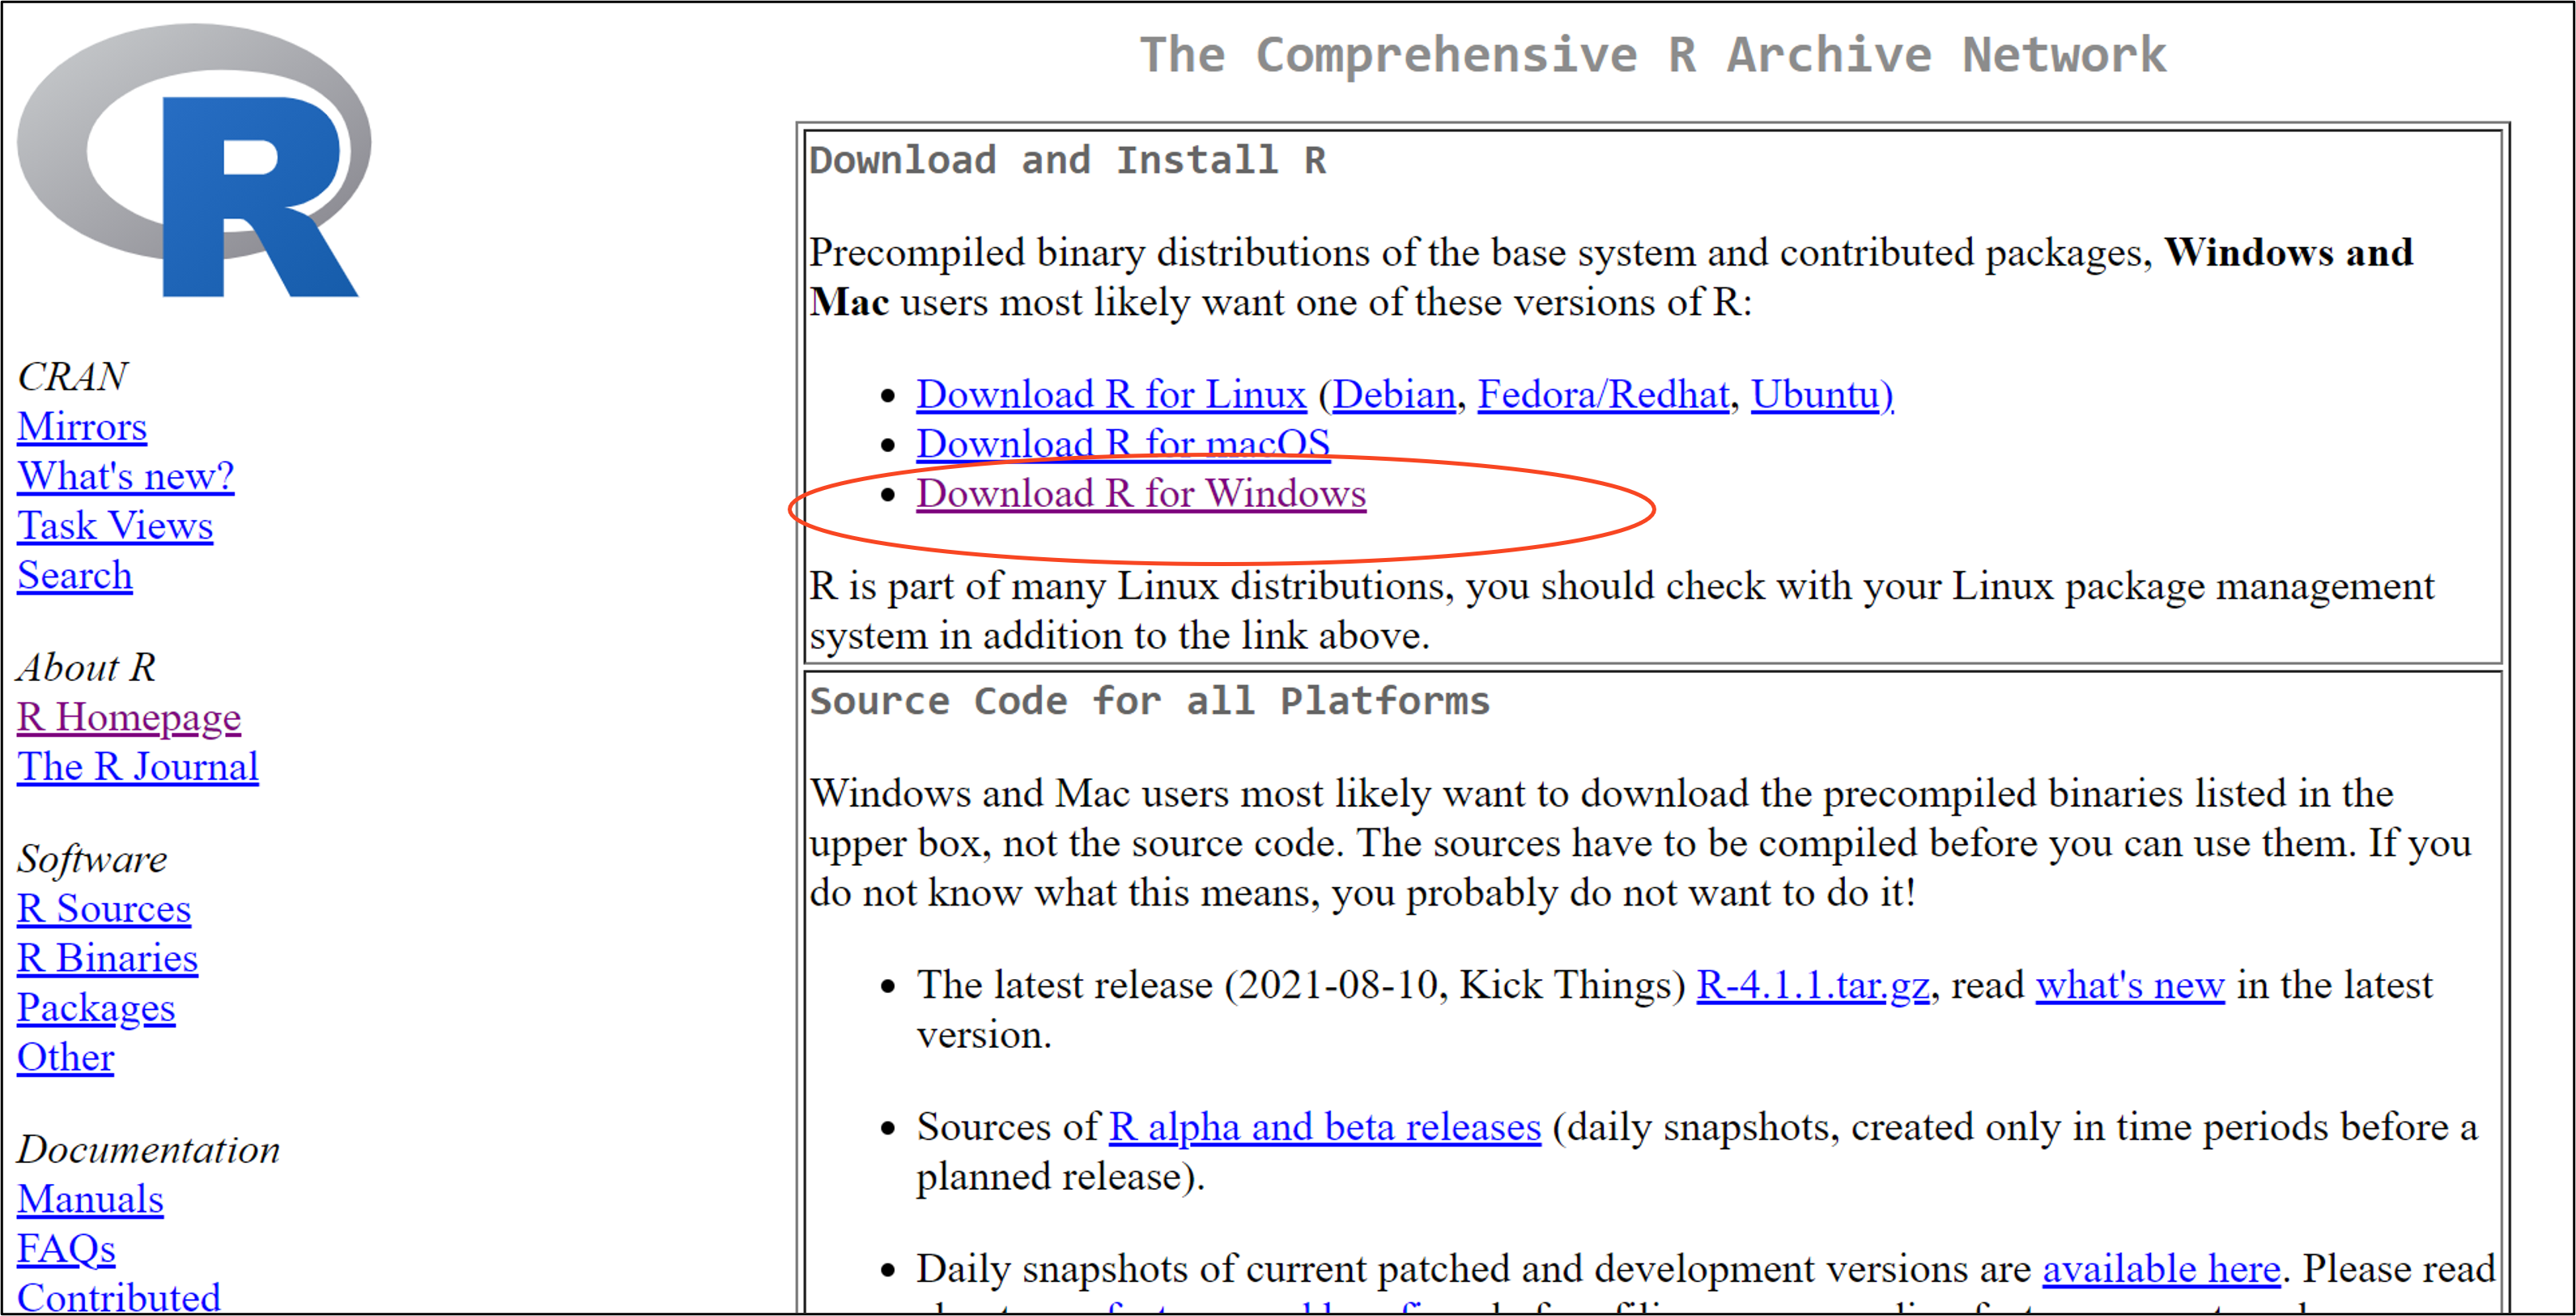
\includegraphics{tutorial_screenshots/download_r.png}\\
3. On the next window click on `install R for the first time'

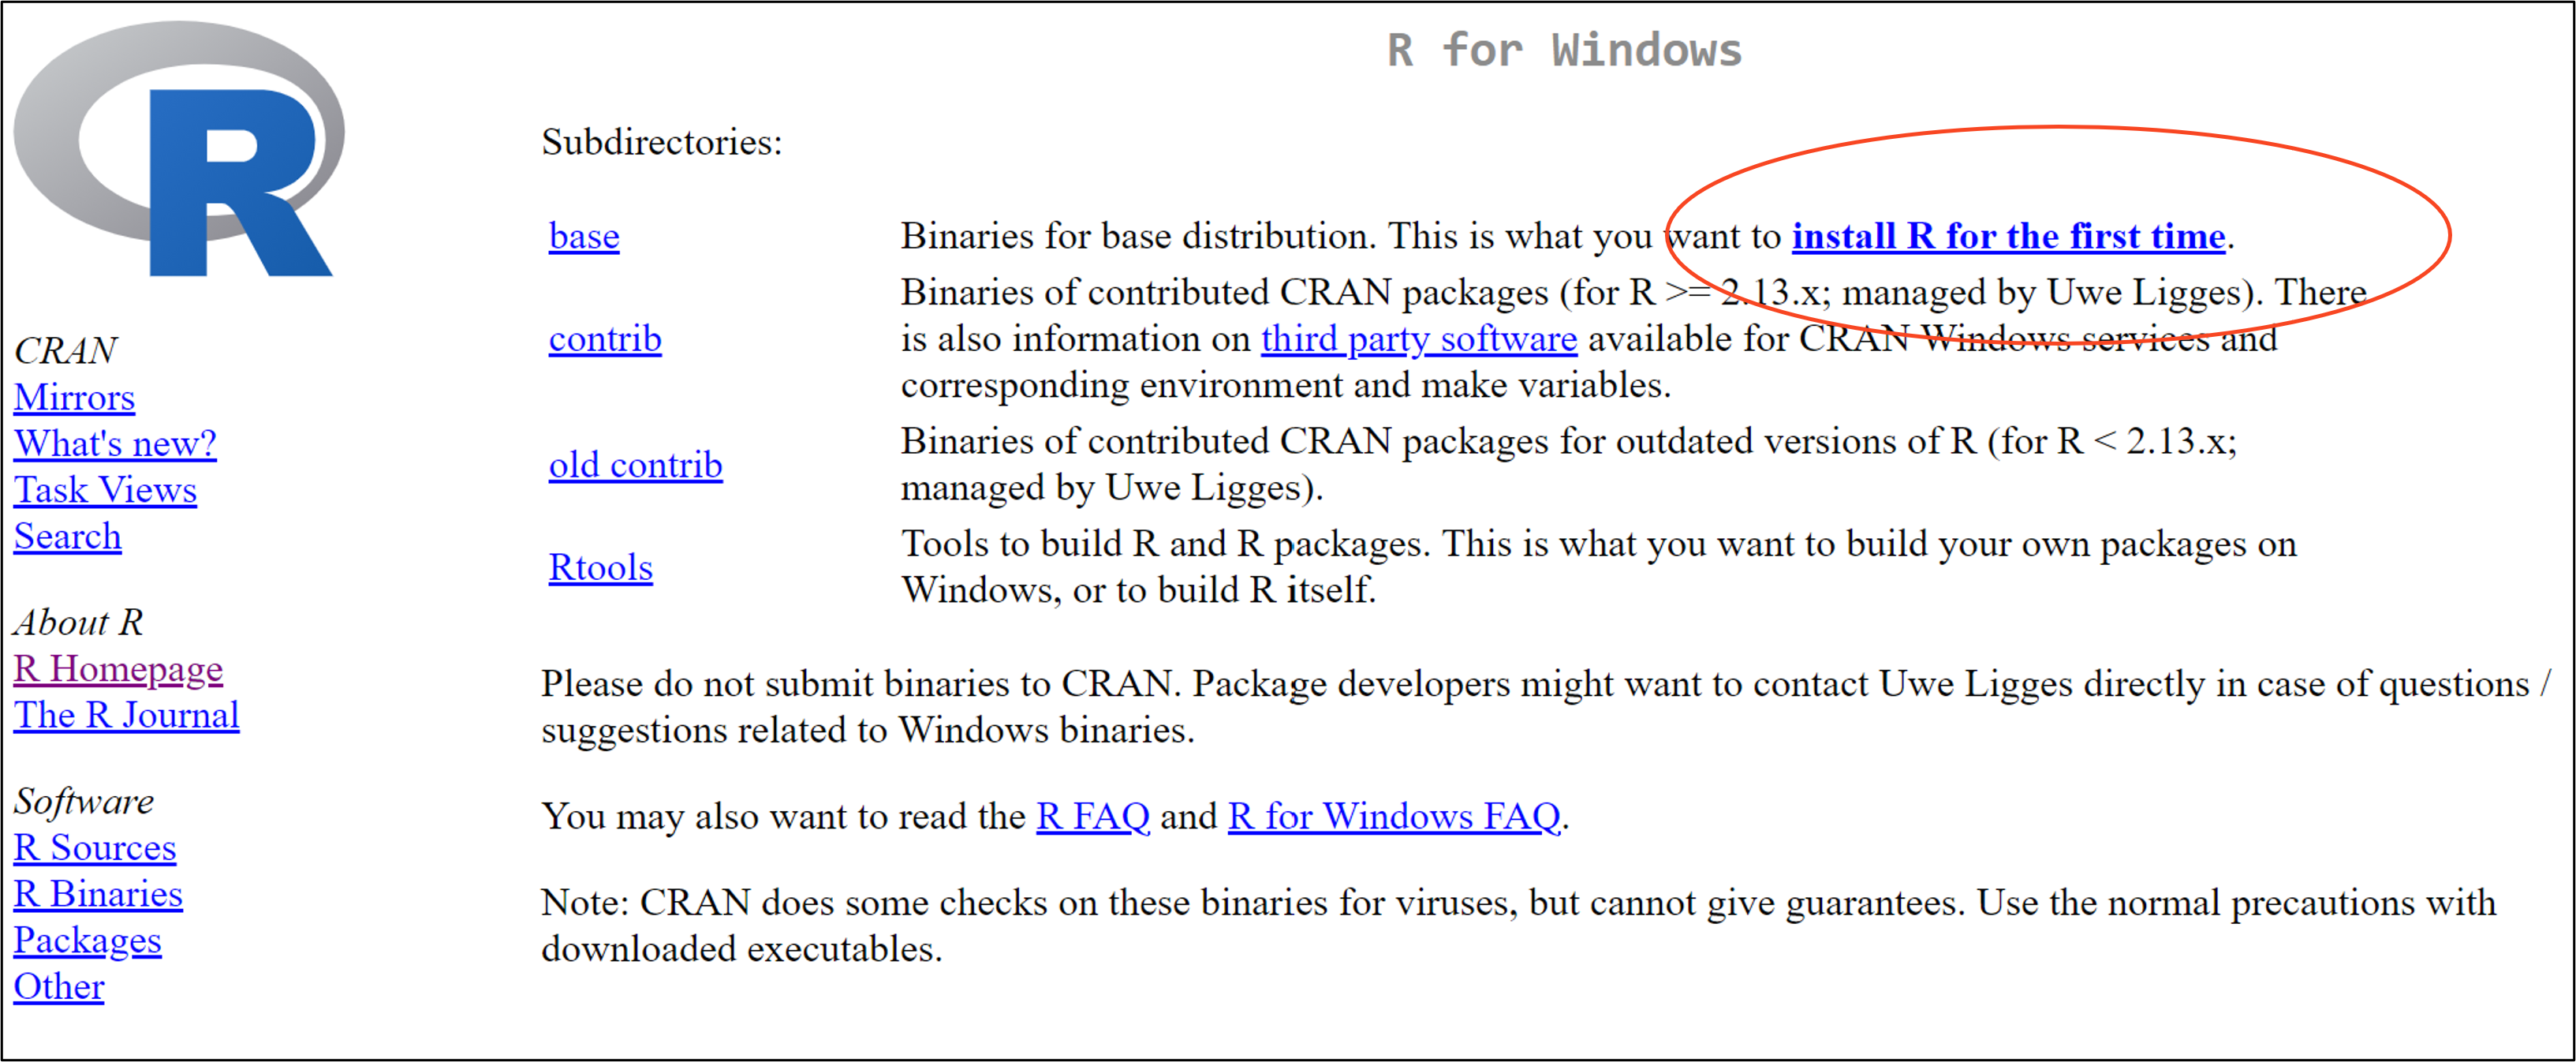
\includegraphics{tutorial_screenshots/install_r1.png}

\begin{enumerate}
\def\labelenumi{\arabic{enumi}.}
\setcounter{enumi}{3}
\tightlist
\item
  Click on `Download R x.x.x for windows'
  \textgreater{} x.x.x = current R version
\end{enumerate}

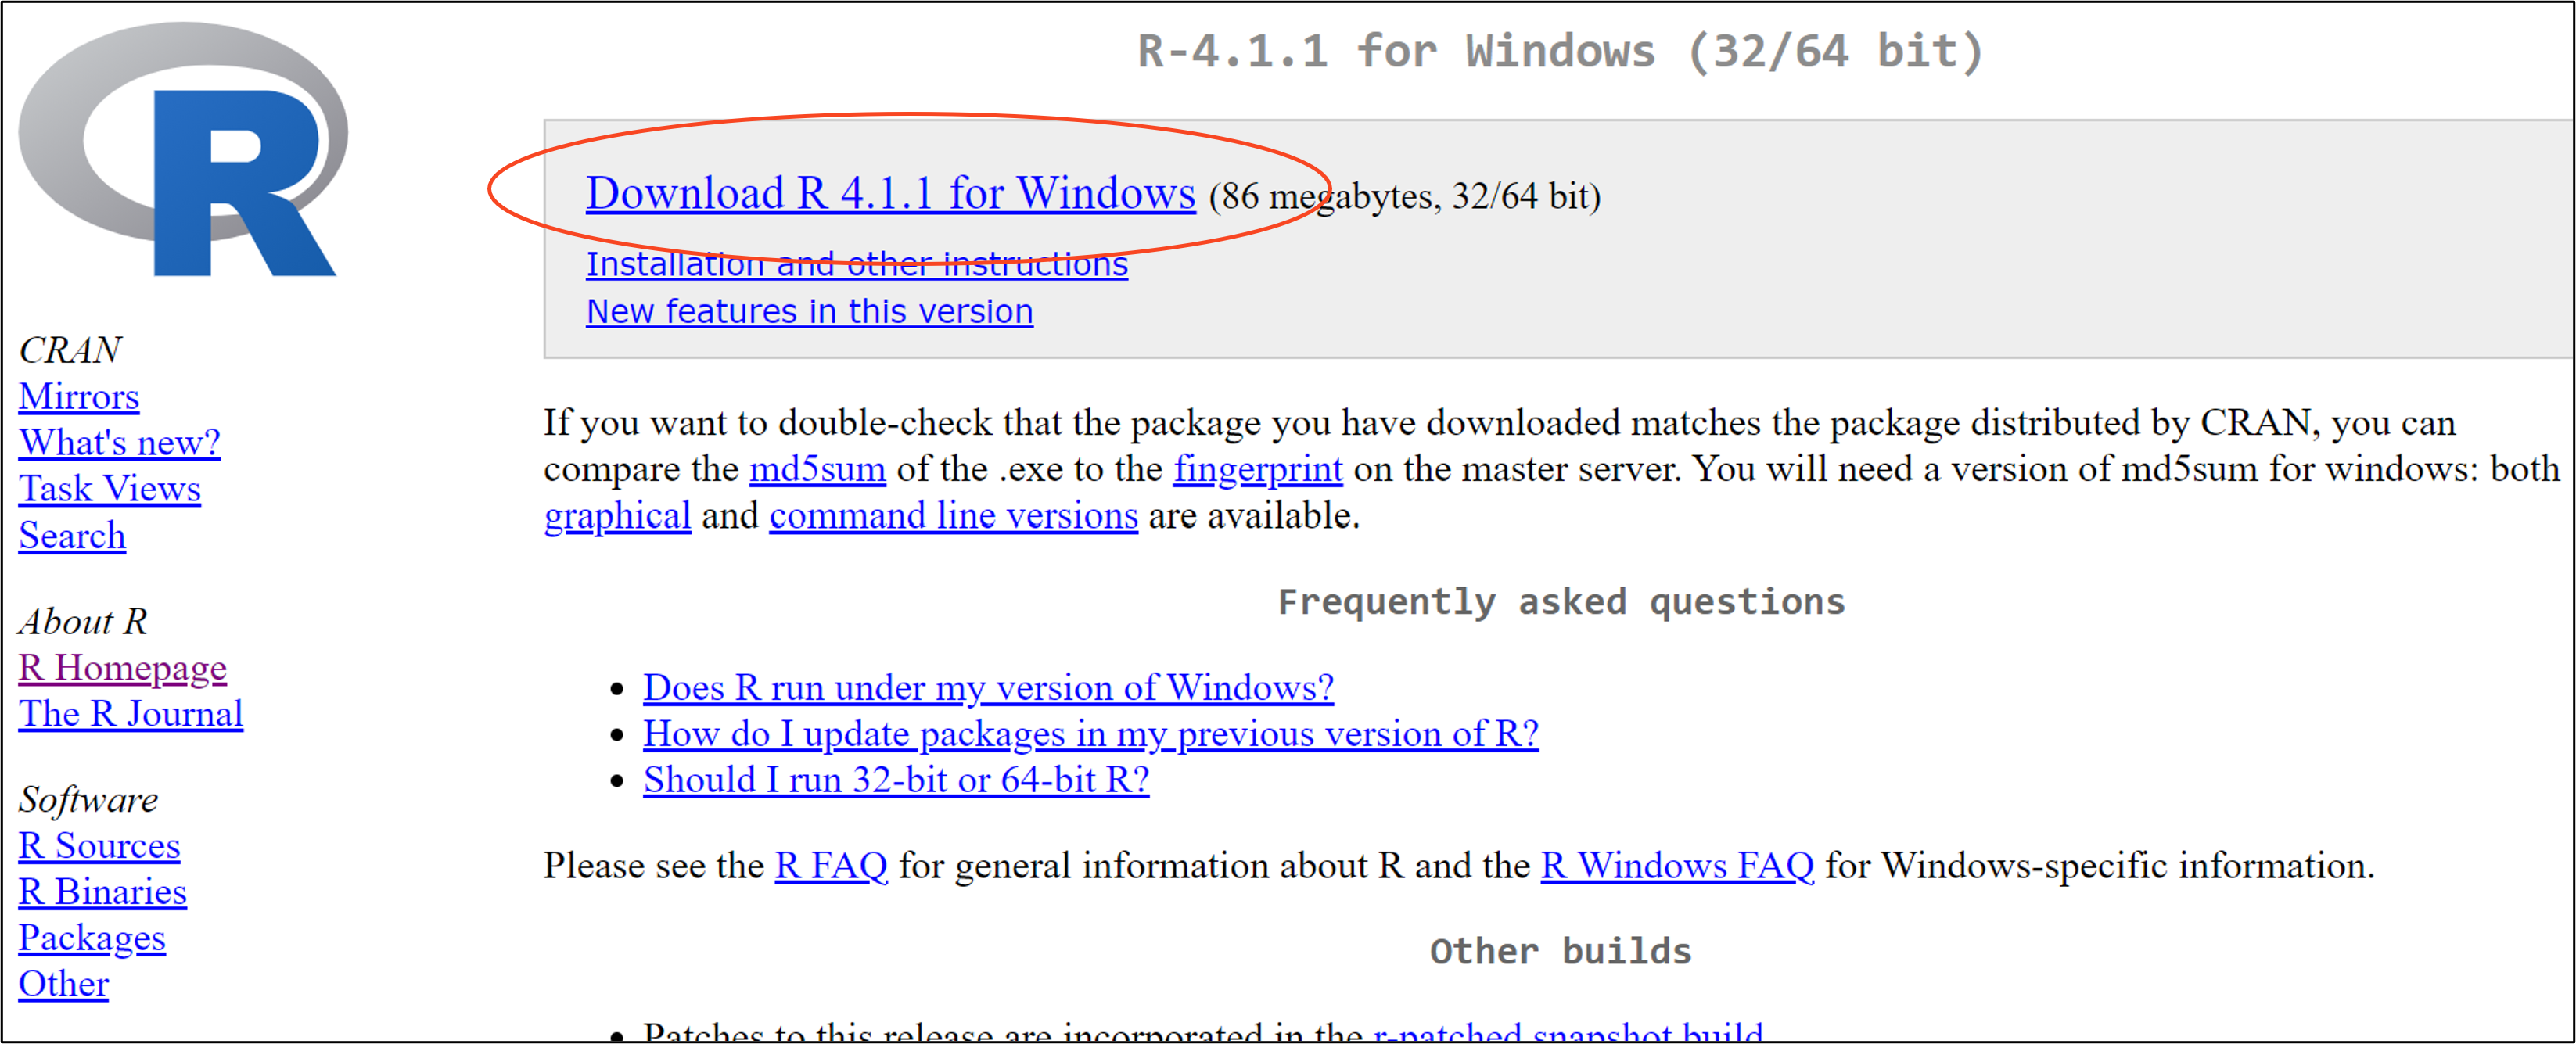
\includegraphics{tutorial_screenshots/download_r_current.png}

\begin{enumerate}
\def\labelenumi{\arabic{enumi}.}
\setcounter{enumi}{4}
\tightlist
\item
  Navigate to your download folder and run the .exe file that you downloaded and follow the installation prompts\\
\item
  When prompted to `select components to install', select all\\
  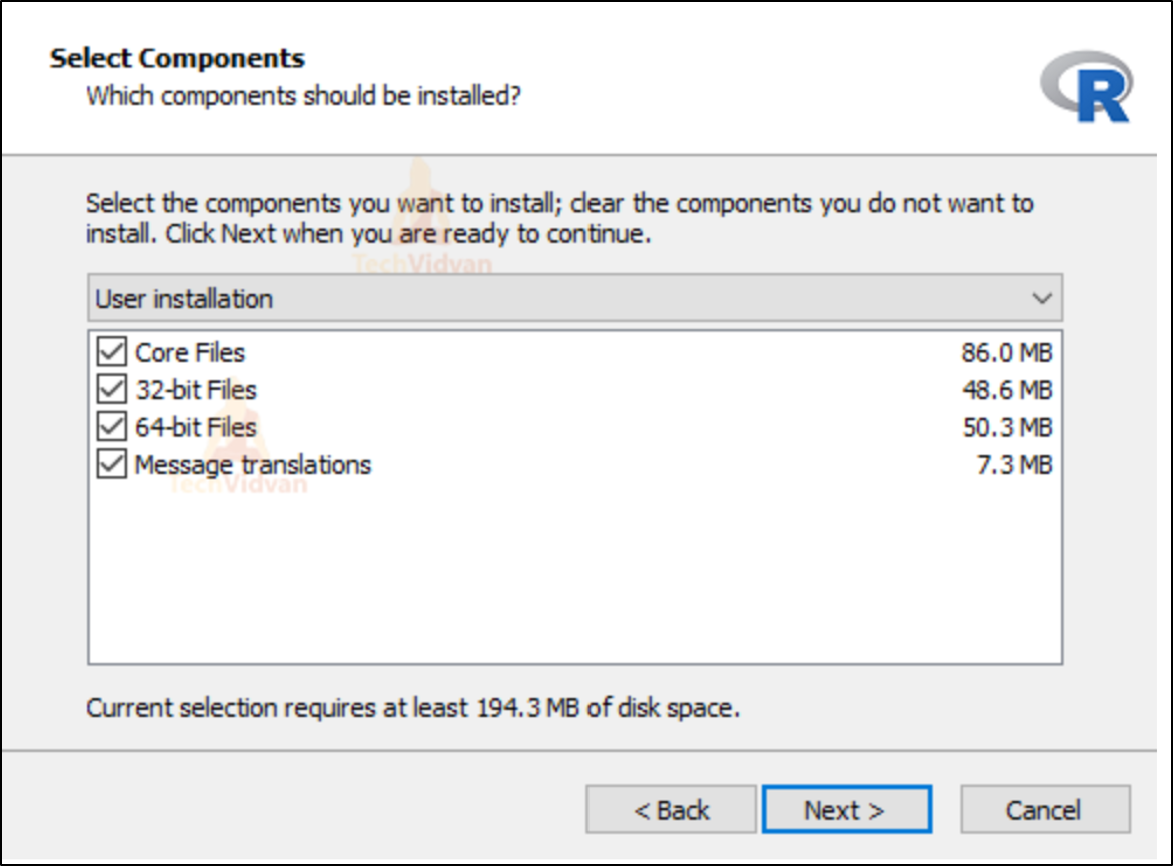
\includegraphics{tutorial_screenshots/install_r_components.png}
\end{enumerate}

\hypertarget{install-rstudio}{%
\subsection{Install RStudio}\label{install-rstudio}}

\begin{enumerate}
\def\labelenumi{\arabic{enumi}.}
\tightlist
\item
  Go to \href{https://www.rstudio.com/products/rstudio/download/}{}\\
\item
  Click on the download button for free version of RStudio Desktop (or any other desired version)
\end{enumerate}

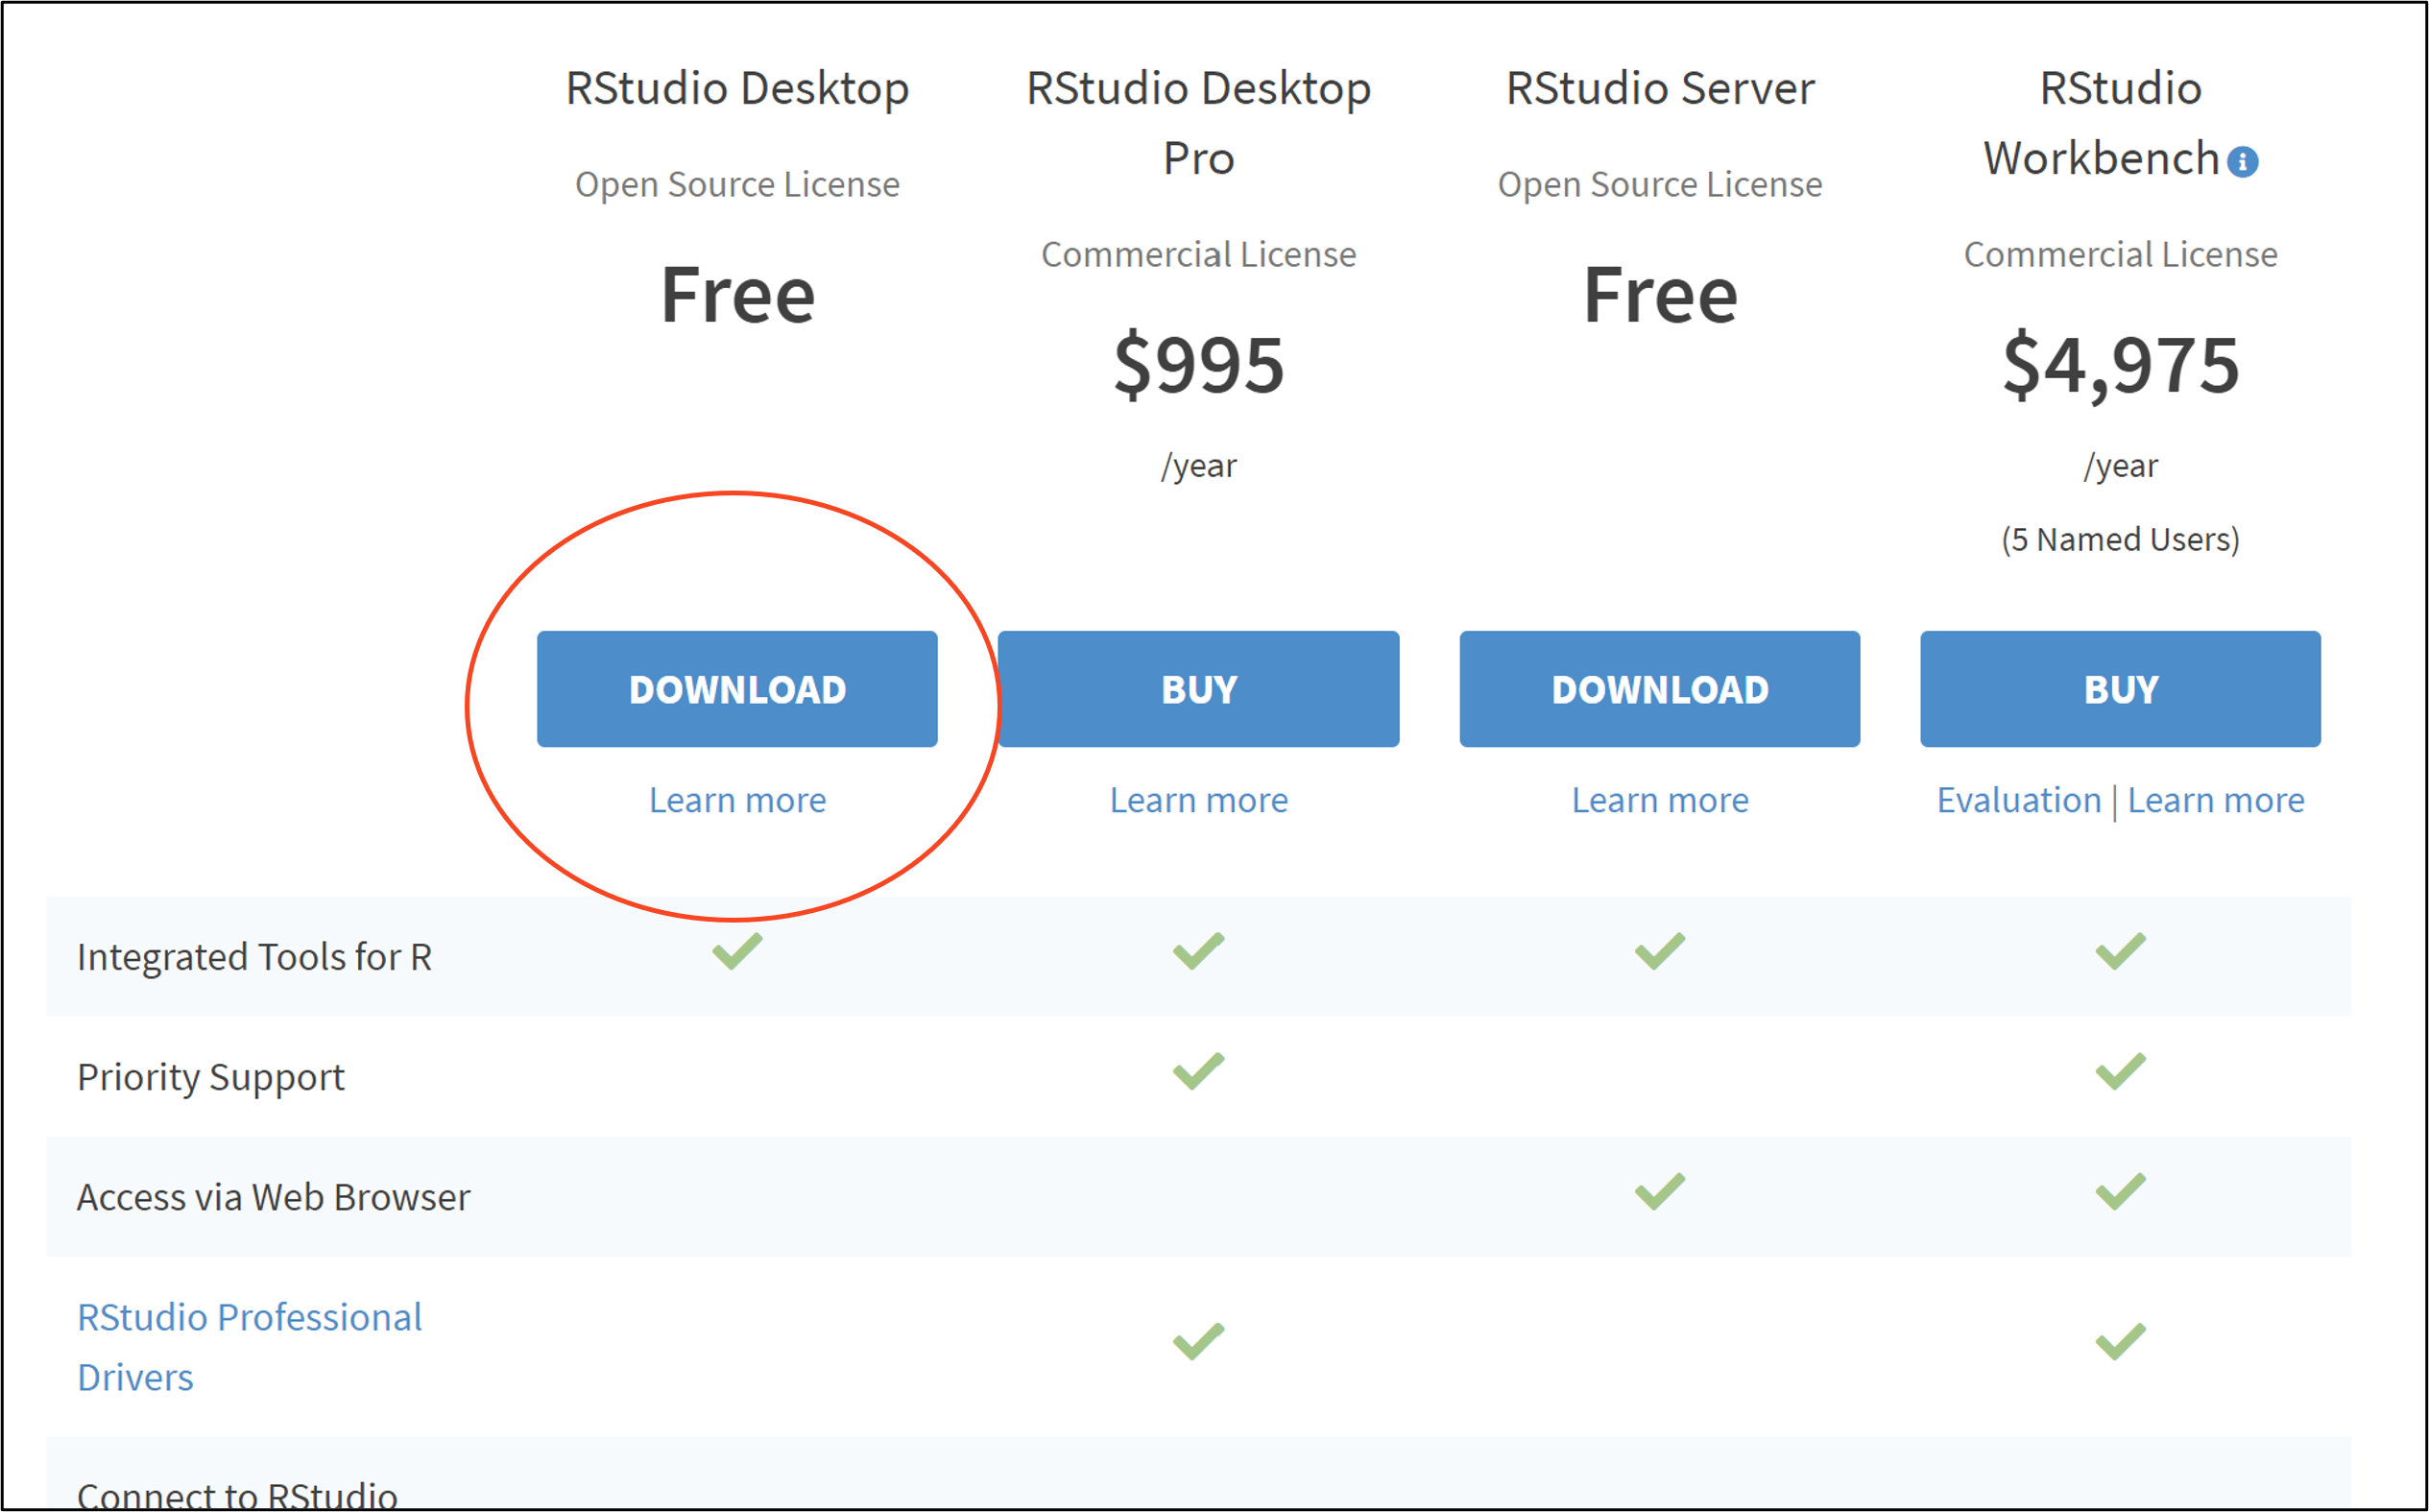
\includegraphics{tutorial_screenshots/download_rstudio.png}

\begin{enumerate}
\def\labelenumi{\arabic{enumi}.}
\setcounter{enumi}{2}
\tightlist
\item
  Click on `DOWNLOAD RSTUDIO FOR WINDOWS'
\end{enumerate}

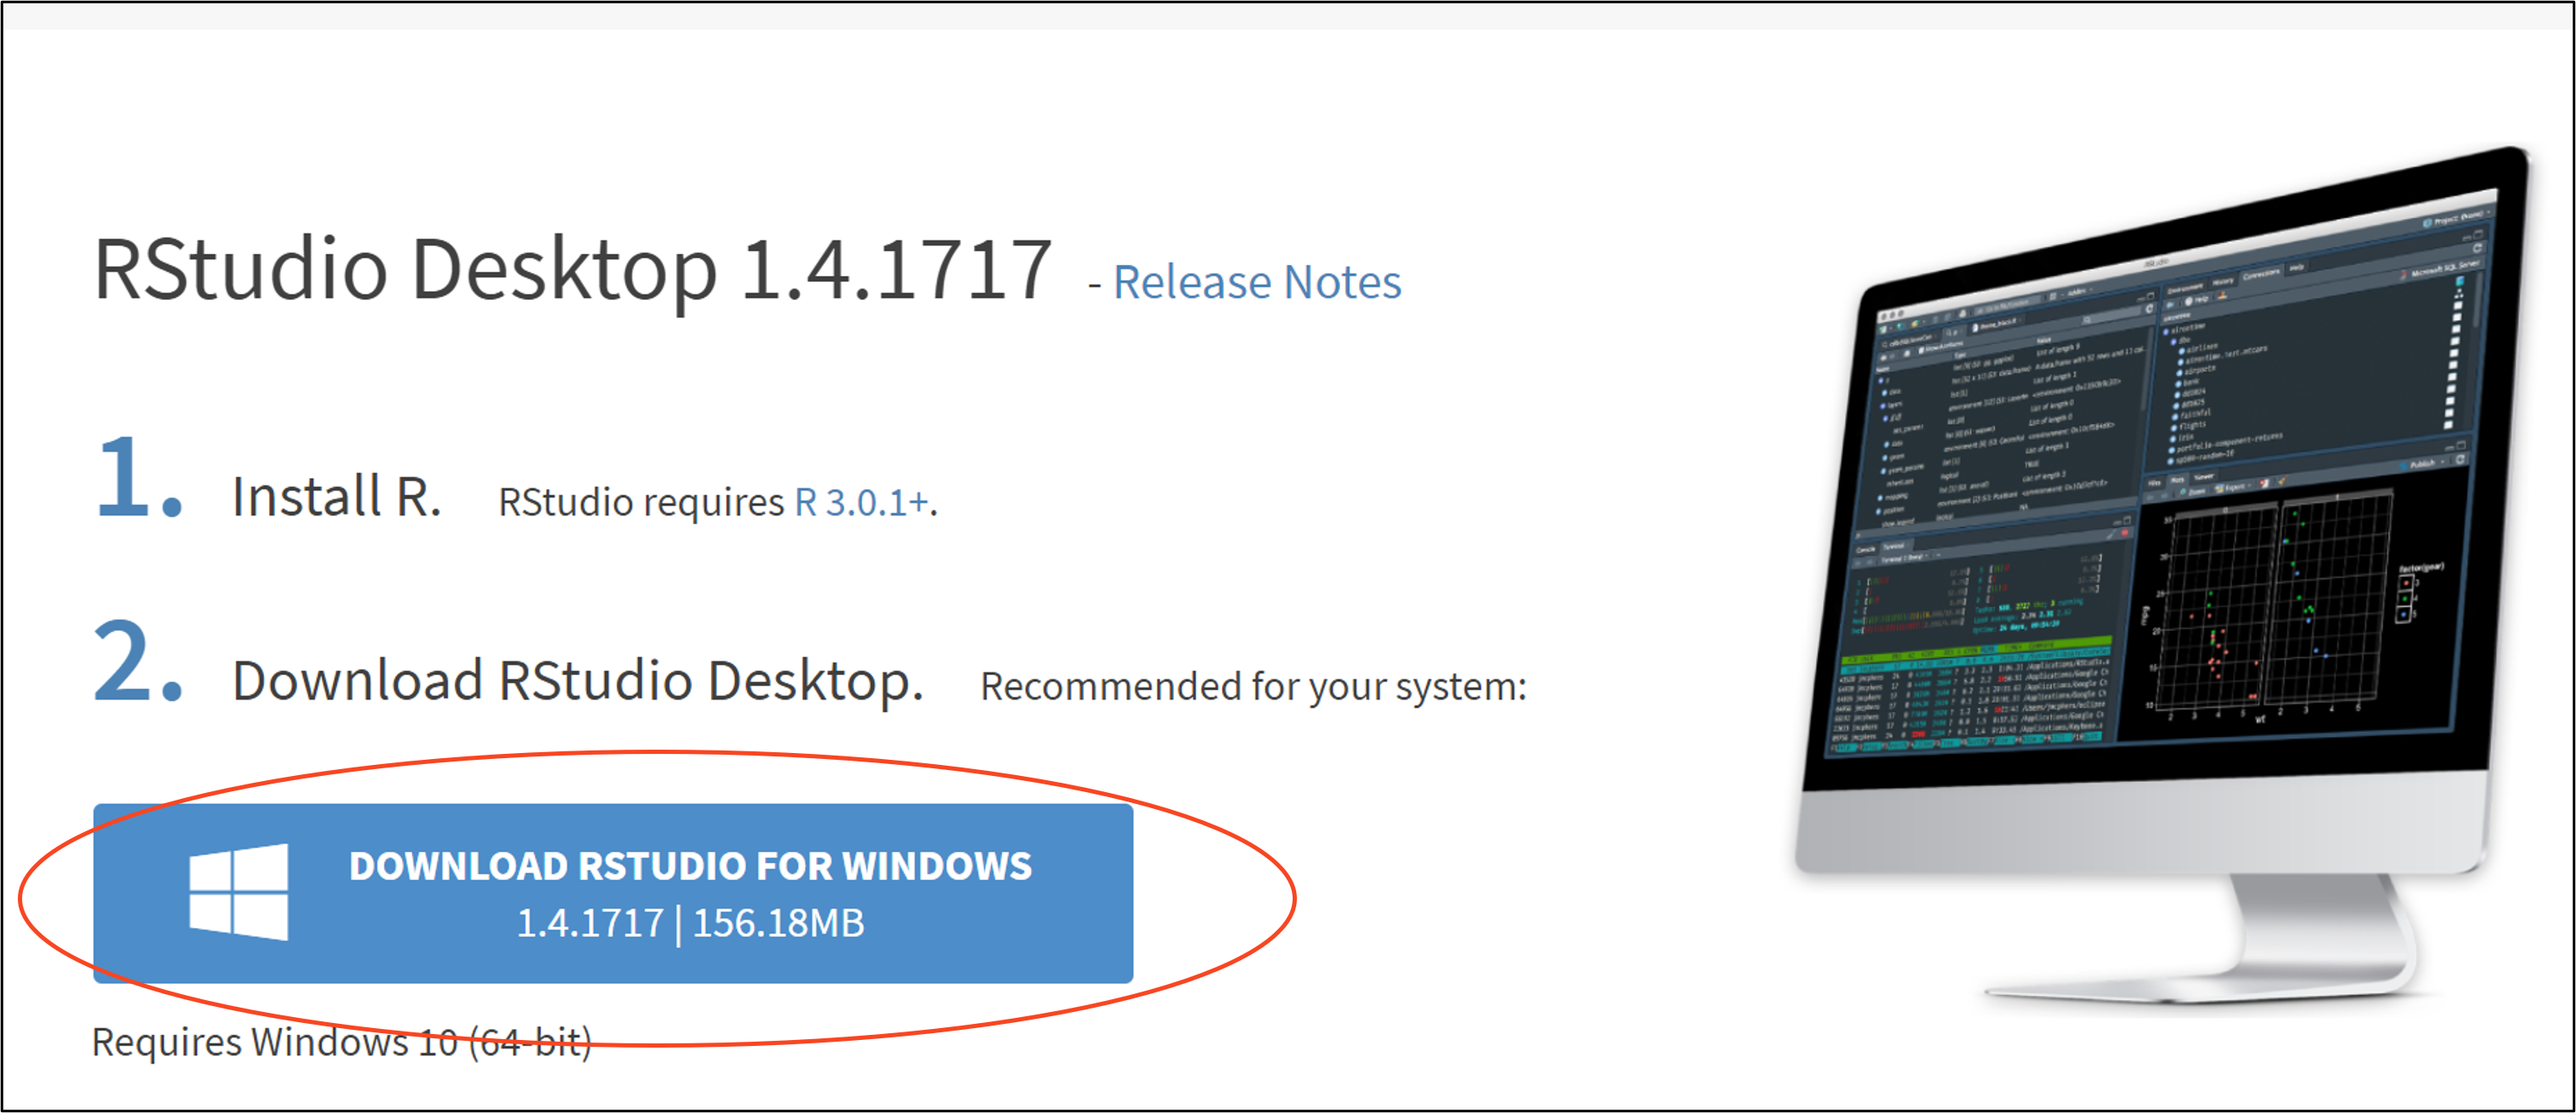
\includegraphics{tutorial_screenshots/download_rstudio2.png}

\begin{enumerate}
\def\labelenumi{\arabic{enumi}.}
\setcounter{enumi}{3}
\tightlist
\item
  Run the .exe file that you downloaded and follow the installation prompts
\end{enumerate}

\emph{Most of the installation settings may be left as default}

\hypertarget{signing-up-on-github}{%
\subsection{Signing up on GitHub}\label{signing-up-on-github}}

\begin{enumerate}
\def\labelenumi{\arabic{enumi}.}
\tightlist
\item
  Go to \href{https://github.com/}{}\\
\item
  Enter you email address\\
\item
  Click 'Sign up for GitHub
\end{enumerate}


\includegraphics{tutorial_screenshots/gh_signup.png}

\begin{enumerate}
\def\labelenumi{\arabic{enumi}.}
\setcounter{enumi}{2}
\tightlist
\item
  Follow the prompts to create a password and username
\end{enumerate}

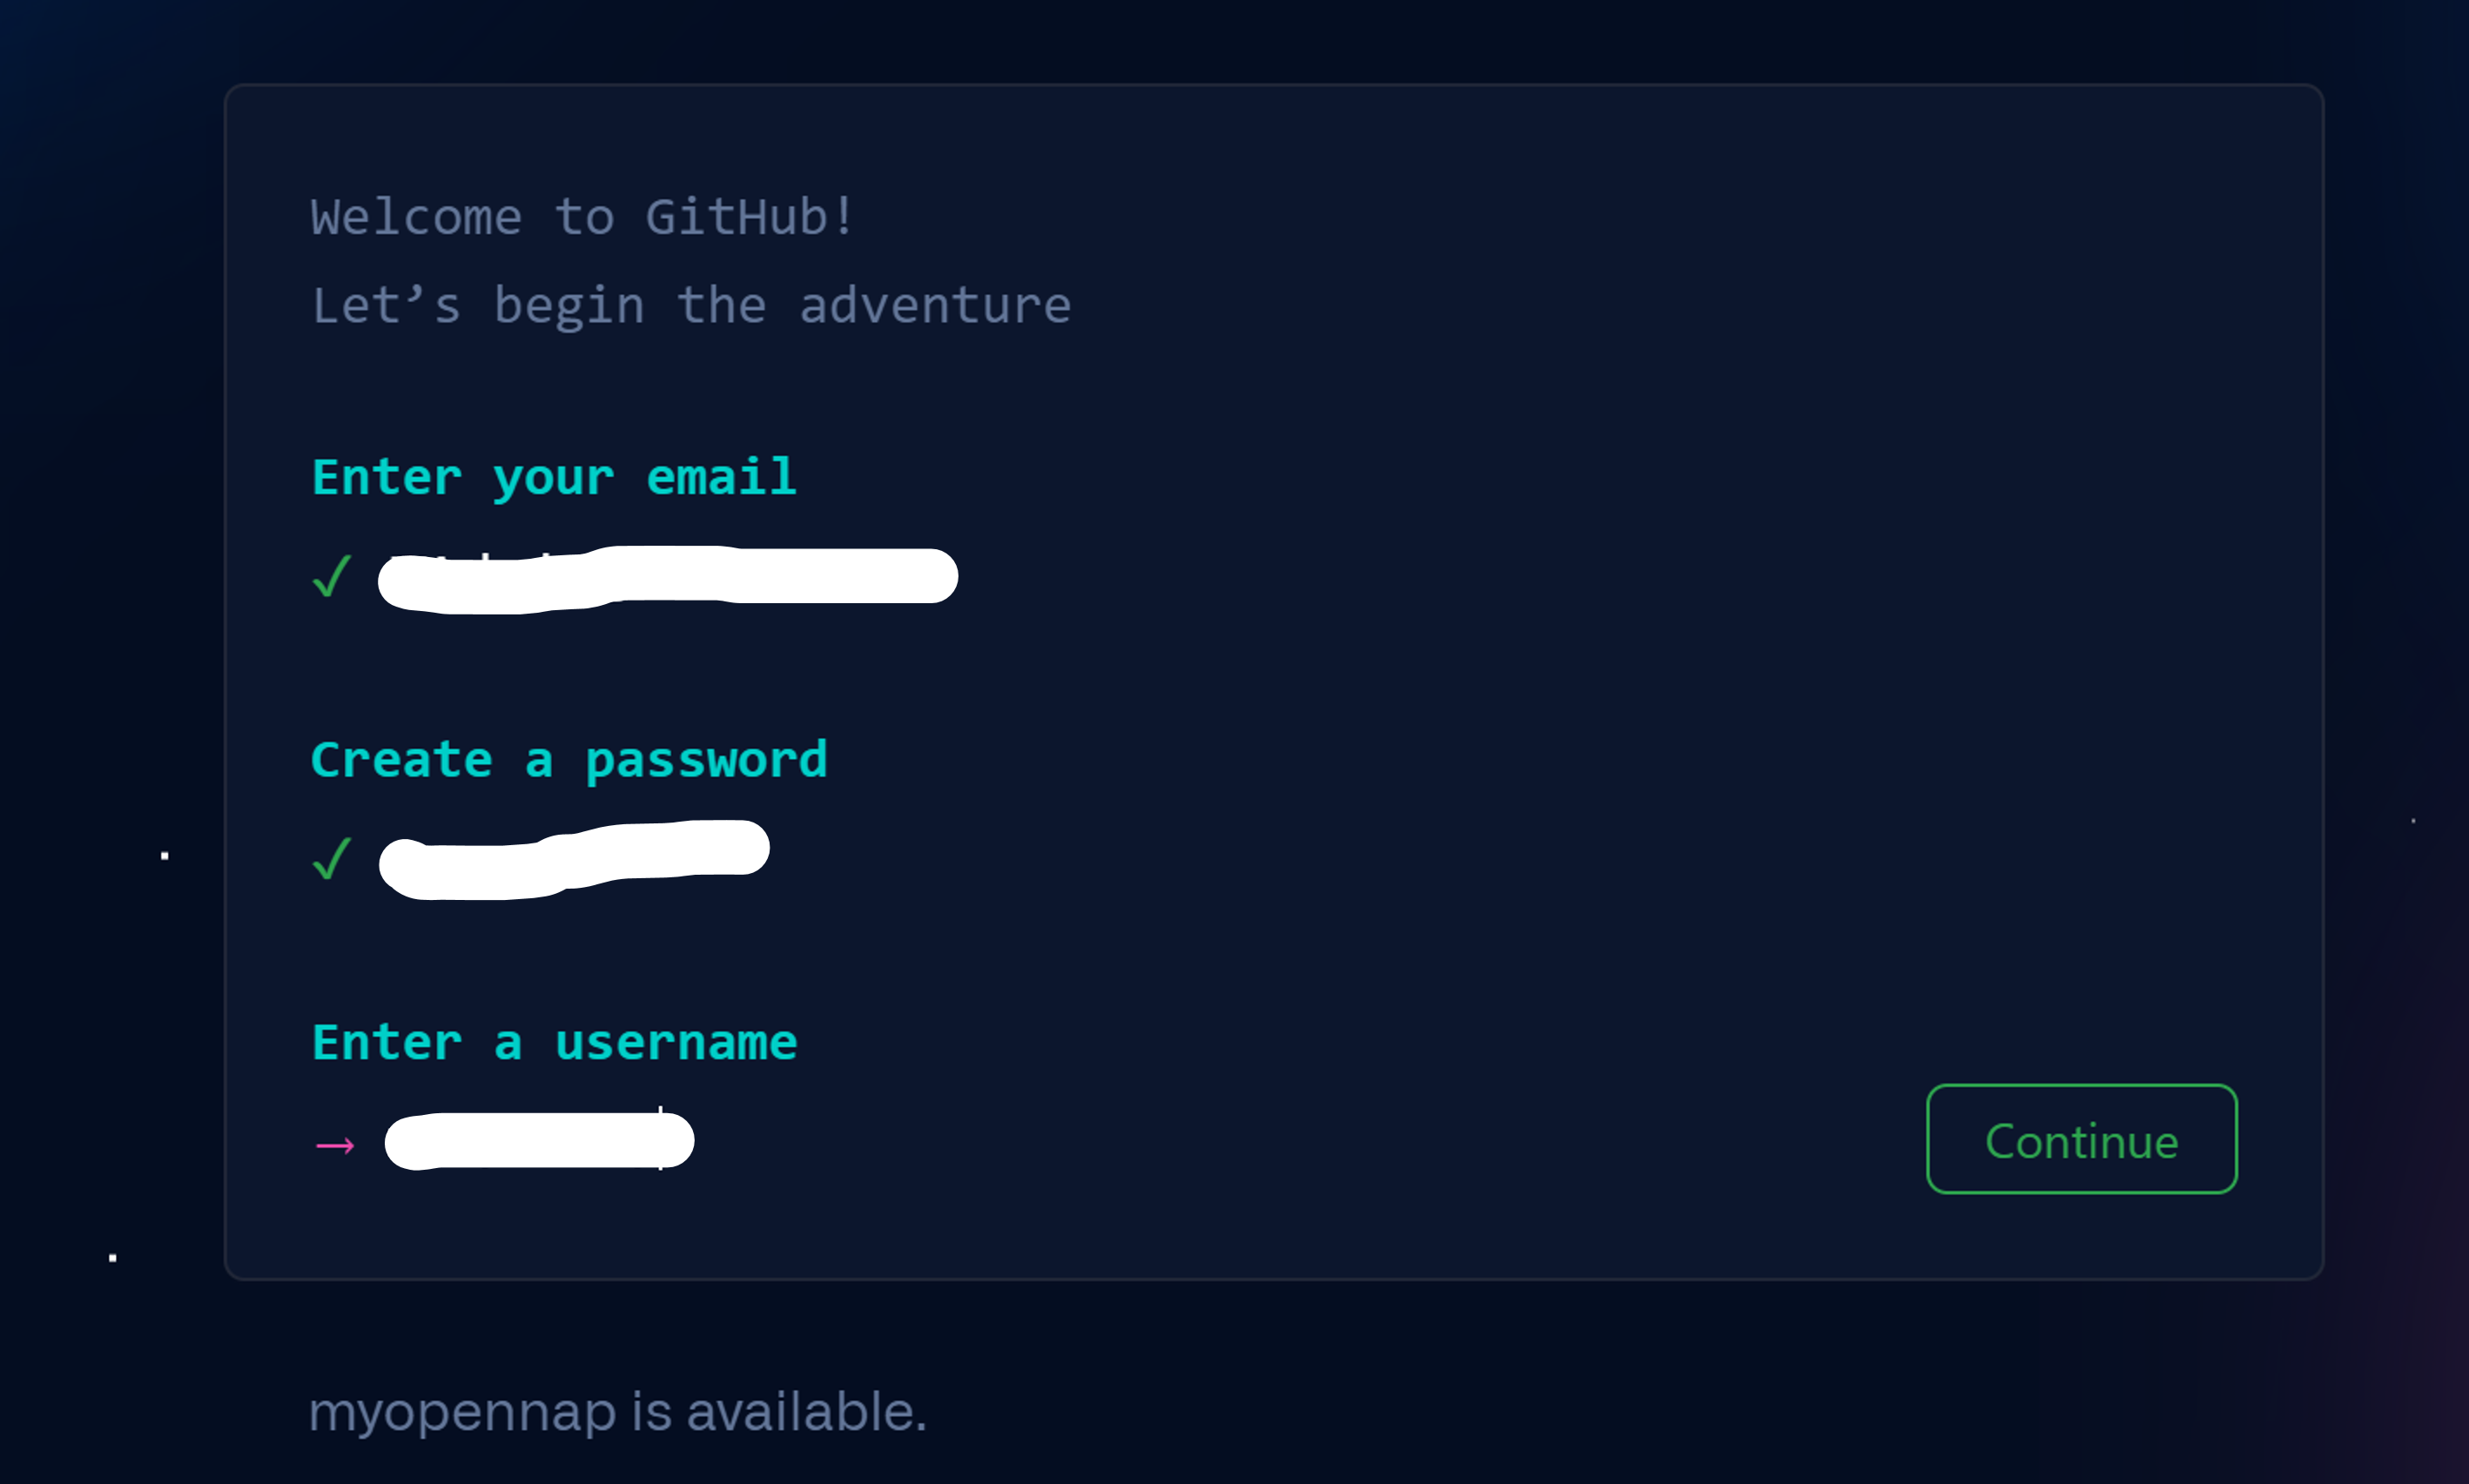
\includegraphics{tutorial_screenshots/gh_set_profile.png}

\begin{enumerate}
\def\labelenumi{\arabic{enumi}.}
\setcounter{enumi}{3}
\tightlist
\item
  Continue with the prompts to verify identity and email and finish set up
\end{enumerate}

\hypertarget{opening-a-markdown-file}{%
\section{Opening a markdown file}\label{opening-a-markdown-file}}

\begin{enumerate}
\def\labelenumi{\arabic{enumi}.}
\tightlist
\item
  Launch your r/studio app.
  Your rstudio workspace should look more or less similar to this:
\end{enumerate}

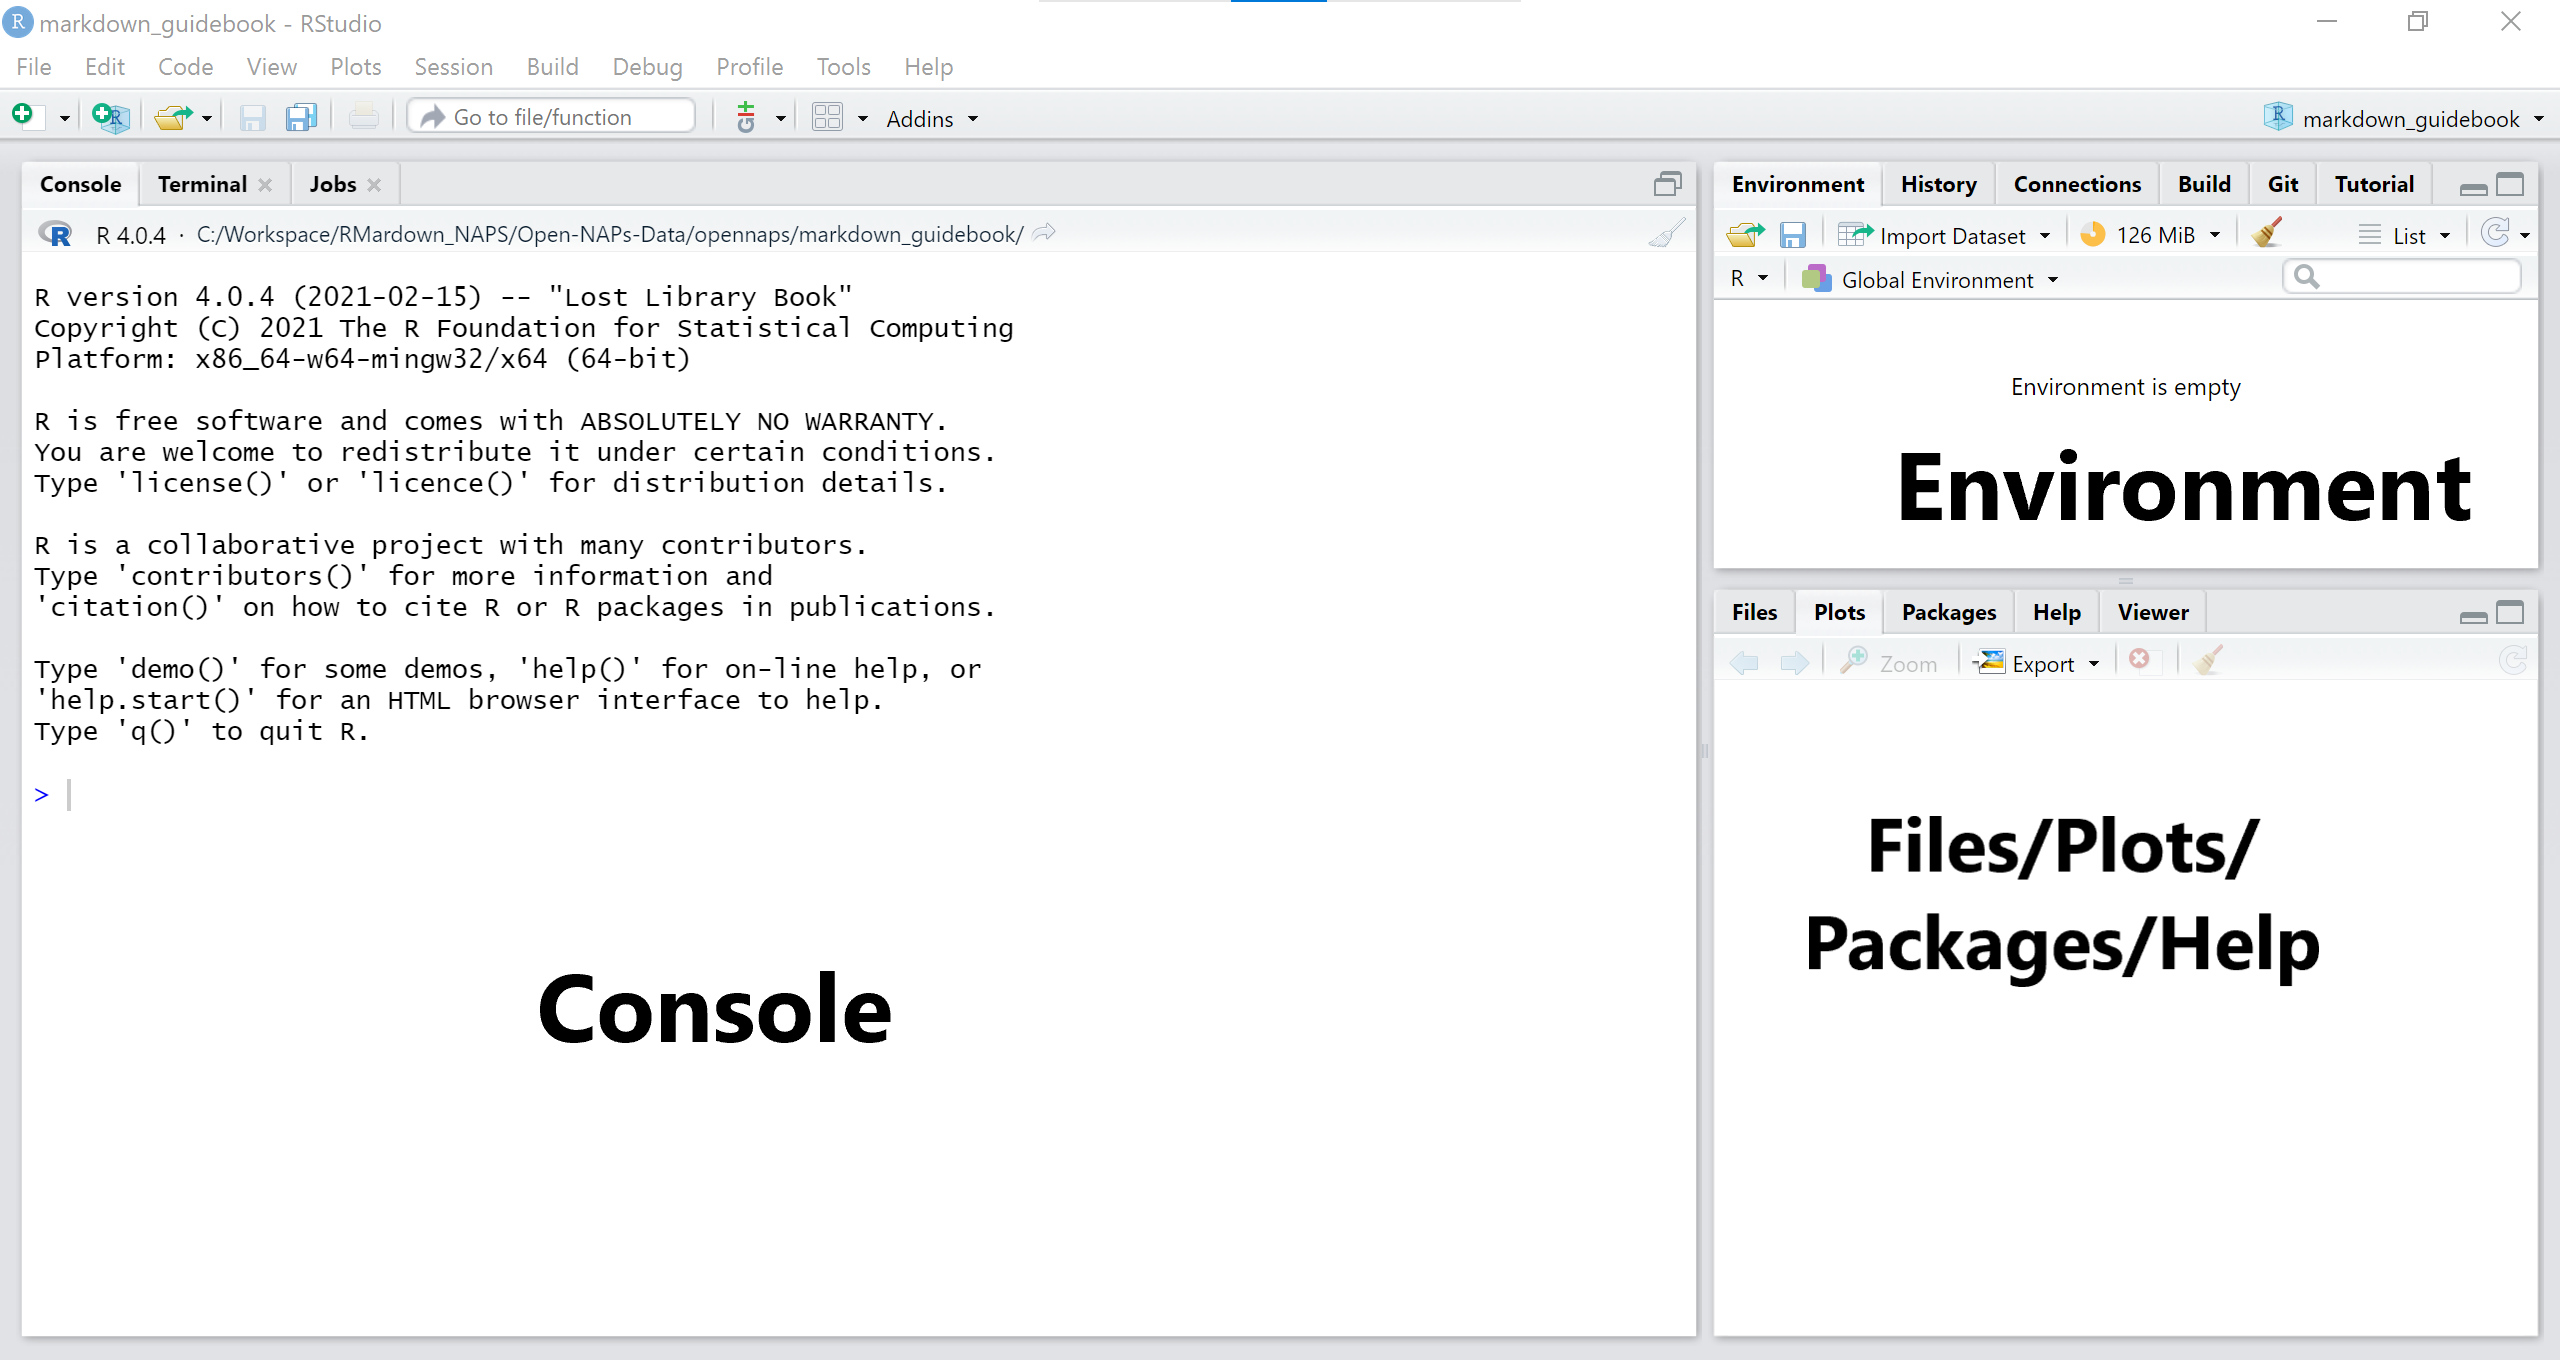
\includegraphics{tutorial_screenshots/rstudio_panels.png}\\
If your rstudio opens up with 4 windows instead of 3, skip next step.\\
2. From the main menu, go to File-\textgreater\textgreater New File-\textgreater\textgreater R Markdown.\\
You should have a window like this:\\
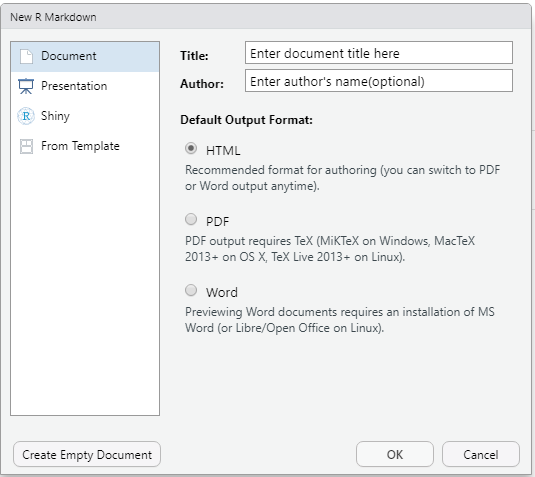
\includegraphics{tutorial_screenshots/open_rmd_file.png}\\
3. Fill in the details for your document title and author. Leave the rest as default.\\
4. Click Ok.\\
This opens up your 4th rstudio window with an rmarkdown script.\\
Now your app area should look more or less like this;\\
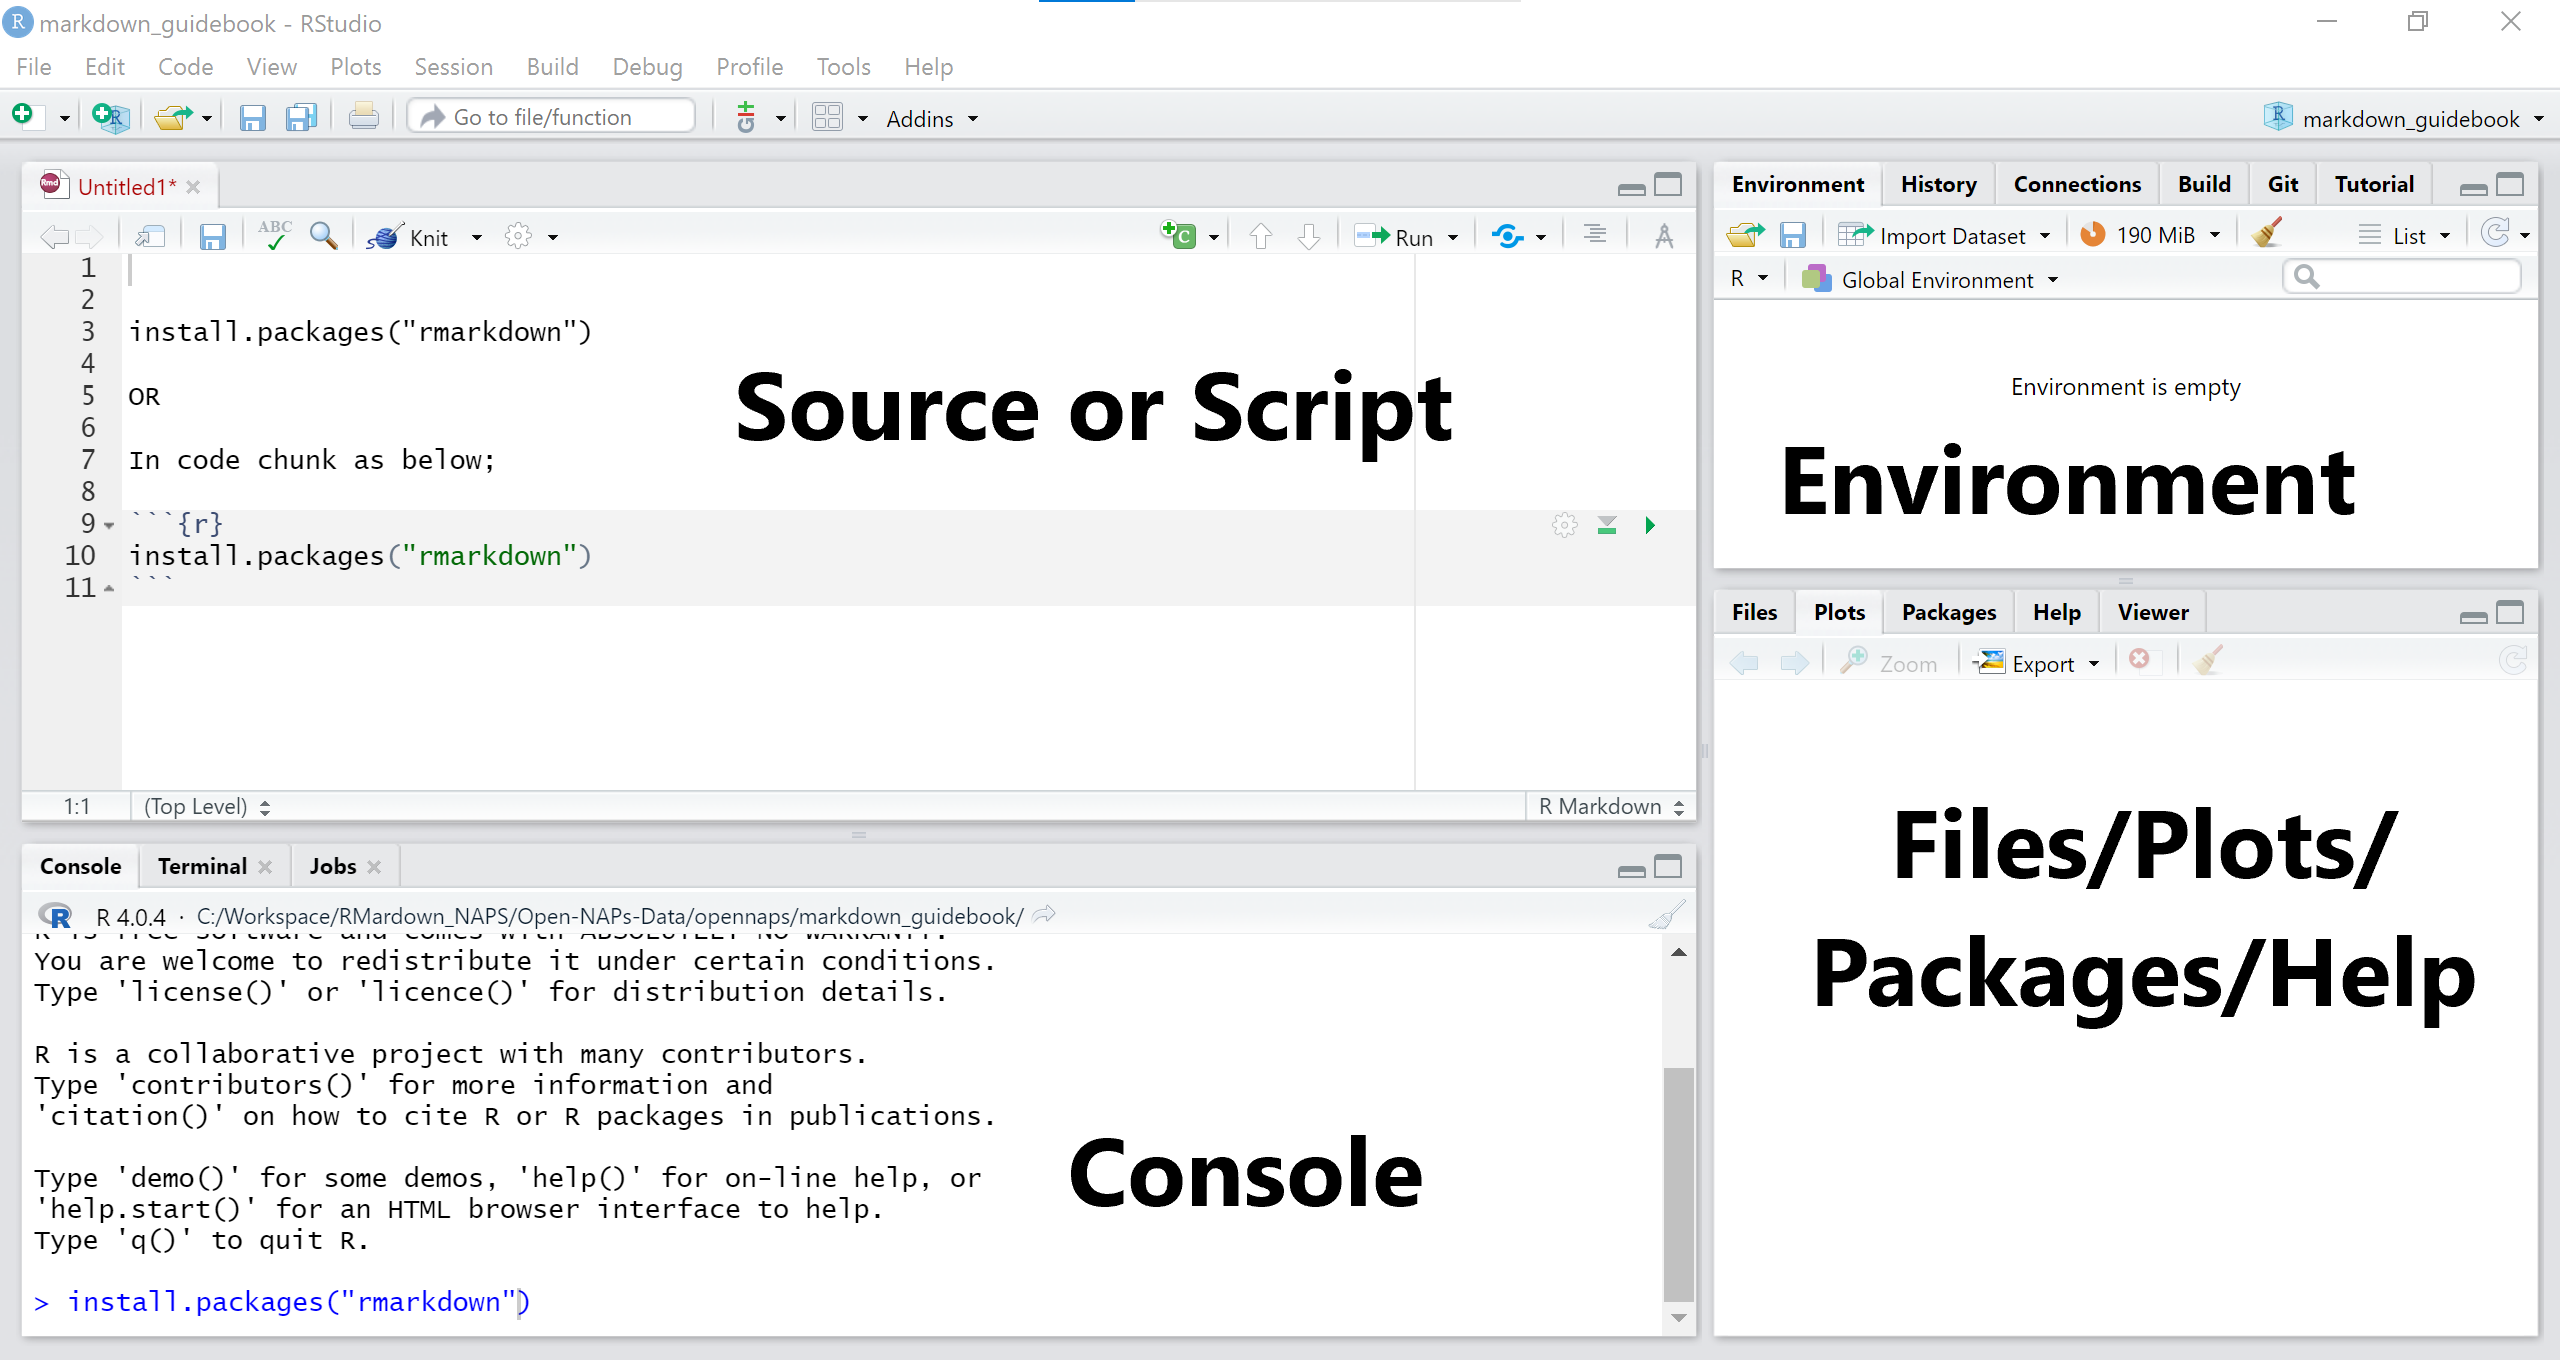
\includegraphics{tutorial_screenshots/rstudio_panels_4.png}

The arrangement may however be different. If so, do not worry, it's just semantics.

\emph{As you might have seen, you may open other scripts such as R, python, SQL etc in similar manner.}

\hypertarget{rstudio-windows-explained}{%
\subsection{Rstudio windows explained:}\label{rstudio-windows-explained}}

\begin{itemize}
\item
  \textbf{The Source}\\
  This is your scripting area.\\
  You may write, edit and run your code from here.
\item
  \textbf{The Console}\\
  All processing in r happens here. You may this is the r kitchen.
  When you run your code, this is where it is evaluated.\\
  You may also use the console to write and execute your code. However, you can not save your code, nor can you edit it (you will have to rewrite it). Thus, it is always advisable to write your code in the script/source area.\\
\item
  \textbf{The Environment}\\
  This panel holds your data objects and their metadata. As you create or add new objects into your project, they will appear in this window. You may view and remove objects.
  It also contains the `History' tab from which you may view all your r processing history.\\
\item
  \textbf{The Files/Plots/Packages/Help Panel}\\
  This panel provides a shortcut/alternative to different functions such as to access your project files, to view plots from your code evaluations, install packages and access the Help resource. You may add/remove items here but we will learn that much later. For now we leave it as is.
\end{itemize}

\hypertarget{installing-packages}{%
\section{Installing packages}\label{installing-packages}}

Options:

\textbf{1. From the console}\\
After the greater than (\textgreater) sign, write command \texttt{install.packages("package\ name")} and hit enter on your keyboard.\\
See example;

\begin{figure}
\centering
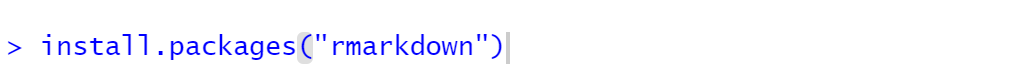
\includegraphics{tutorial_screenshots/install_rmkdn_console.png}
\caption{install packages from console}
\end{figure}

\textbf{2. In script window }\\
Inside your script write command \texttt{install.packages("package\ name")}\\
Click on `Run' (Run button is on the top right of your source panel).\\
Alternatively, if your write your command in a code chunk, you may hit the `Play' button on far right of your code chunk. See example;

\begin{figure}
\centering
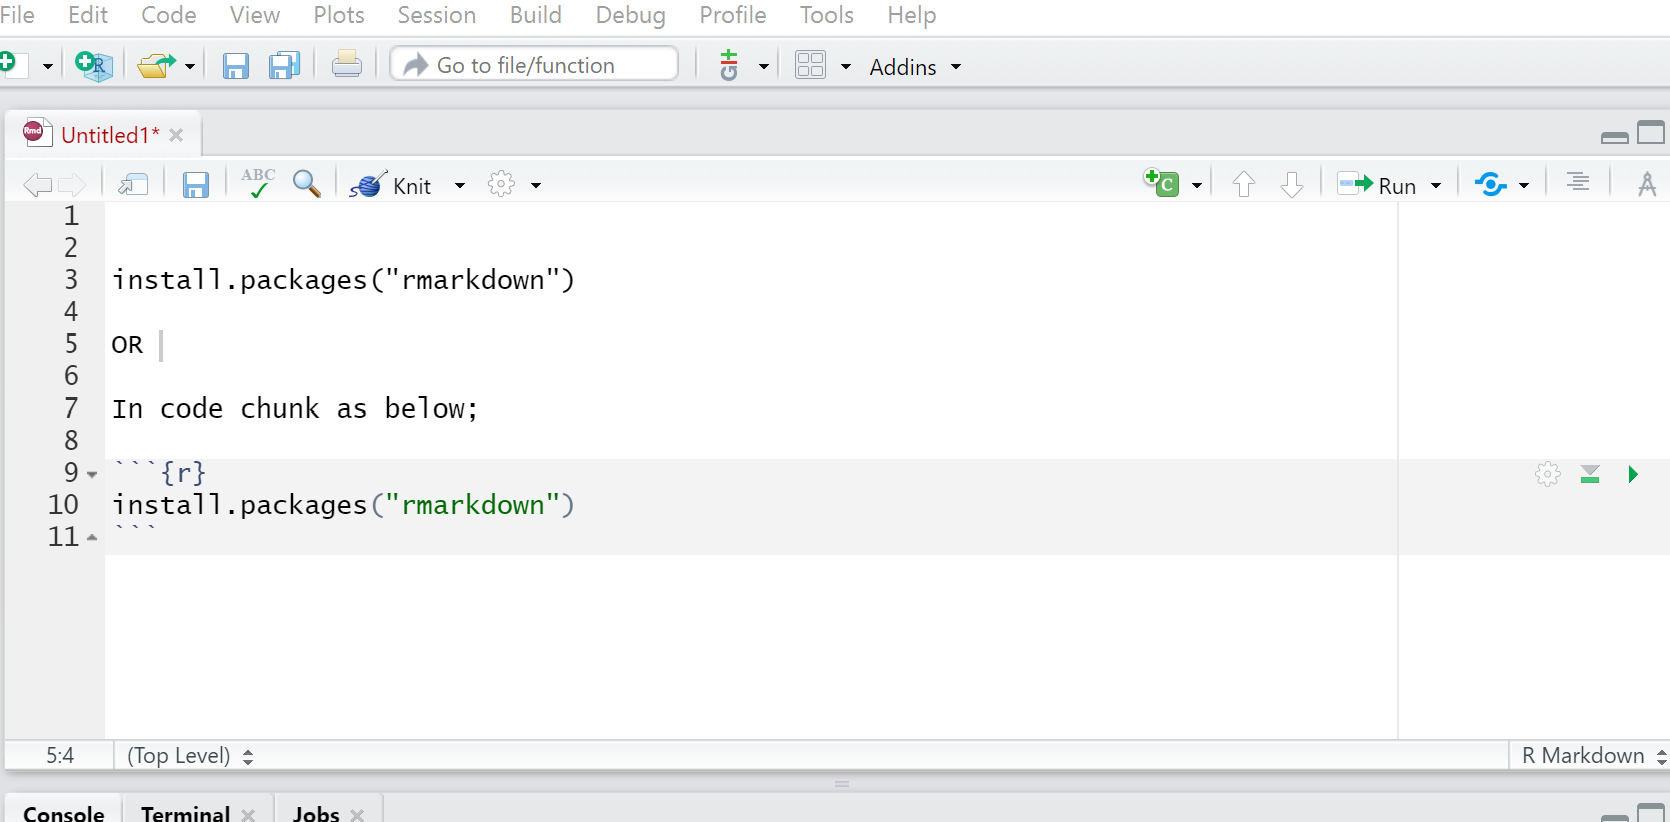
\includegraphics{tutorial_screenshots/install_rmkdn_scrpt.png}
\caption{install packages from script wnindow}
\end{figure}

*We see more about code chunks in the next chapter.

\textbf{3. From the menu bar }\\
From the menu bar, go the the tab `Tools' and select `Install Packages'.\\
You should see a window like this one:

\begin{figure}
\centering
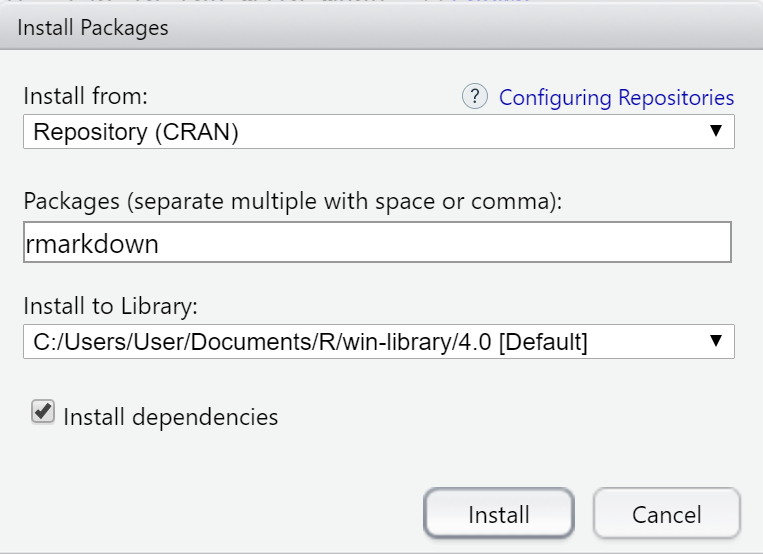
\includegraphics{tutorial_screenshots/install_rmkdn_toolstab.png}
\caption{install packages from menu bar}
\end{figure}

In the `Install from' field, select `Repository (CRAN)', then enter the name(s) of packages to be installed.\\
Leave everything else as default. Click Install.

\textbf{4. From Files/Plots/Packages/Help Panel}\\
Click on the `Packages' tab. There are 2 tabs under this, Install \& Update.\\
Click on Install.

\begin{figure}
\centering
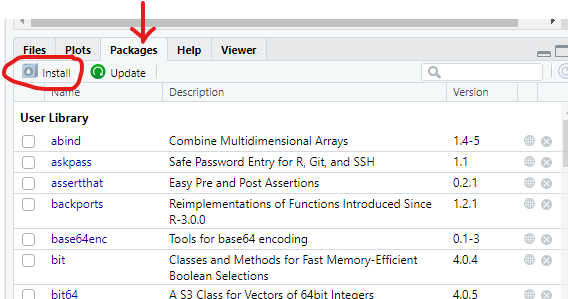
\includegraphics{tutorial_screenshots/install_packages_short.png}
\caption{install packages}
\end{figure}

If the `Install from' is not set to `Repository (CRAN)', set it so, and enter name(s) of packages to be installed.\\
Leave everything else as default. Click Install.

\textbf{Note:Packages can only be installed once. To mean, if you close your r/rstudio app and come back to it the next day/session, you do not need to install the packages you already installed in your previous session. You will only need to load their libraries (see next section)}

\hypertarget{removingun-installing-packages}{%
\subsection{Removing/un-installing packages}\label{removingun-installing-packages}}

To remove a package use command \texttt{remove.packages("package\ name")}

\begin{figure}
\centering

\includegraphics{tutorial_screenshots/remove_package.png}
\caption{remove packages}
\end{figure}

\hypertarget{loading-libraries}{%
\section{Loading Libraries}\label{loading-libraries}}

To be able to make use of the packages installed, you need to call their libraries. Most libraries take the name of the package. For instance, for the package \texttt{rmakdown}, the respective library is \texttt{rmarkdown}.To call the rmarkdown library, use command \texttt{library(rmarkdown)}.
So in general to load/call libraries use command \texttt{library(name\ of\ library)}.

\begin{figure}
\centering

\includegraphics{tutorial_screenshots/load_library.png}
\caption{load library}
\end{figure}

You may load libraries in the console or in your script.

\textbf{Note:Unlike packages,library functions expire when you close a project or end a session. Therefore, each time you open an r session, you have to load/call relevant libraries}

\hypertarget{getting-started-1}{%
\chapter{Getting started}\label{getting-started-1}}

\hypertarget{about-rmarkdown}{%
\section{About RMarkdown}\label{about-rmarkdown}}

RMarkdown is a file document that allows you to write, save and execute code, as well as text and figures to help generate reproducible reports that can be shared in several formats.
The file extension is .rmd.\\
A markdown file has three main sections;

\begin{enumerate}
\def\labelenumi{\arabic{enumi}.}
\item
  \textbf{YAML header}\\
  This is where your document metadata go to e.g your document title, author, date, output file type etc.
  Theses parameters are set when opening a new .rmd or project file. And more can be set after.
  This section MUST always be at the beginning of your document and between a set of three dashes i.e three dashes before section and three dashes after section.
\item
  \textbf{Text}\\
  Your narration/prose in markdown format. More details about formatting in subsequent sections.
\item
  \textbf{Code chunk(s)}\\
  They start with ```\{r\}

  and end with ```
  as in below screenshot
\end{enumerate}

\begin{figure}
\centering
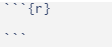
\includegraphics{tutorial_screenshots/codechunk_blank.png}
\caption{code chunk}
\end{figure}

To start using RMarkdown, install the following base packages using any of the methods described in the \protect\hyperlink{installing-packages}{Installing packages} section

\begin{quote}
(`base64enc', `digest', `evaluate', `glue', `highr', `htmltools', `jquerylib', `jsonlite', `knitr', `magrittr', `markdown', `mime',
`rmarkdown', `stringi', `stringr', `tinytex', `xfun', `yaml')
\end{quote}

\hypertarget{editing-in-markdown}{%
\section{Editing in markdown}\label{editing-in-markdown}}

\hypertarget{headers}{%
\subsection{Headers}\label{headers}}

To create headers for your reports/document e.g.~chapters, sub-chapters and so on; use the hash sign `\#' in front of the title. Sequentially increase the number of ``\#' signs to denote subsequent header levels.\\
Insert blank line before each header (except in the beginning of document).

\begin{figure}
\centering
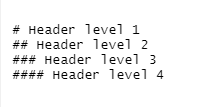
\includegraphics{tutorial_screenshots/headers.png}
\caption{headers}
\end{figure}

\hypertarget{bold-and-italic-text}{%
\subsection{Bold and italic text}\label{bold-and-italic-text}}

To create emphasis in your markdown texts, use an asterisk \texttt{*} before and after text \emph{to italicize} or double asterisk \texttt{**} \textbf{to make your text bold}.\\
Alternatively, you may use single underscore\texttt{\_} \emph{for italics} or double underscore\texttt{\_\_} \textbf{for bold}.

\begin{figure}
\centering
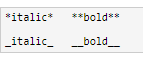
\includegraphics{tutorial_screenshots/italics_bold.png}
\caption{text emphasis}
\end{figure}

\hypertarget{create-lists}{%
\subsection{Create Lists}\label{create-lists}}

\hypertarget{ordered-list}{%
\subsubsection{Ordered list}\label{ordered-list}}

Use numbers to order your list items.
and a plus sign `+' to create sub-items on your list.

\begin{figure}
\centering
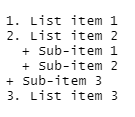
\includegraphics{tutorial_screenshots/ordered_list.png}
\caption{ordered list}
\end{figure}

\hypertarget{unordered-list}{%
\subsubsection{Unordered list}\label{unordered-list}}

Use an asterisk '*' before list item to create an unordered list.\\
Use a plus `+' sign for sub-items.\\
Use tab command or two spaces on your keyboard to indent the list items

\begin{figure}
\centering
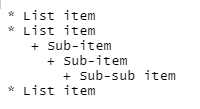
\includegraphics{tutorial_screenshots/unordered_list.png}
\caption{unodered list}
\end{figure}

\textbf{Note: Always leave empty line before starting a new list or use double space or tab on your key board at the end of the text line preceding the list}
As shown in the 2 examples below

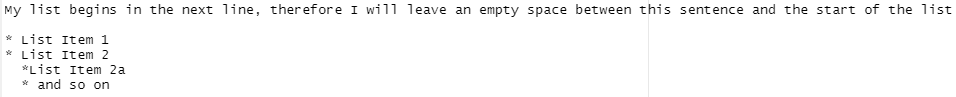
\includegraphics{tutorial_screenshots/listing_empty_space.png}
or

\begin{figure}
\centering
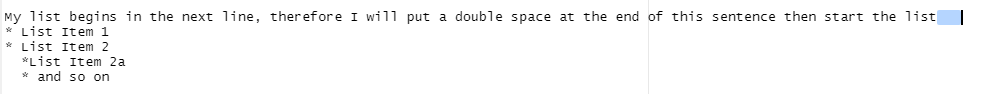
\includegraphics{tutorial_screenshots/listing_space2.png}
\caption{list2}
\end{figure}

\hypertarget{manual-line-breaks}{%
\subsection{Manual line breaks}\label{manual-line-breaks}}

Use two or more spaces at the end of a line\\
to insert a line break

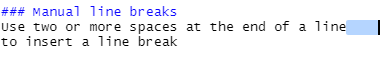
\includegraphics{tutorial_screenshots/line_break.png}
\#\#\# Insert links
You may insert a link using the plain http address such as \url{https://rmarkdown.rstudio.com/} or insert it as a linked phrase using square brackets and parenthesis such as in screenshot


\includegraphics{tutorial_screenshots/link_phrase.png}\\
to produce this:\\
\href{https://rmarkdown.rstudio.com/}{our link phrase goes here}.

\hypertarget{insert-figuresimages}{%
\subsection{Insert figures/images}\label{insert-figuresimages}}

To insert images to our document, we use the same syntax as links, but start with an exclamation mark'!' before syntax.
For an image from a url use; \texttt{!{[}text\ to\ accompany\ your\ image\ e.g\ a\ caption{]}(your\ https\ link)}\\
or for an image file in your local directory use, \texttt{!{[}your\ image\ text{]}(path\ to\ local\ image\ file)}.\\
For instance, I downloaded the UN Climate logo and saved it as a .jpg in my working directory as exact name \texttt{unfccc\_logo.jpg}\\
The following syntax will insert the logo into my document:\\

\includegraphics{tutorial_screenshots/insert_image.png}

\begin{figure}
\centering

\includegraphics{unfccc_logo.jpg}
\caption{UN Climate logo}
\end{figure}

\textbf{When inserting images from local file, it is strongly recommended to have the image in your working directory.}

\hypertarget{insert-block-quotes}{%
\subsection{Insert block quotes}\label{insert-block-quotes}}

To insert a block quote within your text, use the greater than sign `\textgreater{}' in the beginning of quote. The quote must begin on a new line, and remember to insert blank line before and after. For instance the screenshot below;

\begin{figure}
\centering
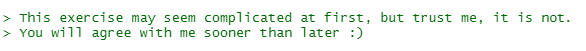
\includegraphics{tutorial_screenshots/block_quote.png}
\caption{block quote}
\end{figure}

produces this:

\begin{quote}
This exercise may seem complicated at first, but trust me, it is not.\\
You will agree with me sooner than later :)
\end{quote}

\hypertarget{insert-code-chunks}{%
\subsection{Insert code chunks}\label{insert-code-chunks}}

To write your code use open code chunk with three backticks
and the curly brackets \{insert your code language\}, hit enter on your keyboard, insert your code and hit enter, close the code chunk with another three backticks.

\begin{figure}
\centering
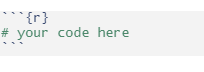
\includegraphics{tutorial_screenshots/code_chunk.png}
\caption{insert code chunk}
\end{figure}

Alternatively, you may do it from top right corner of your script/source window as shown below.
Click on the green +c icon and select R from the drop down list.

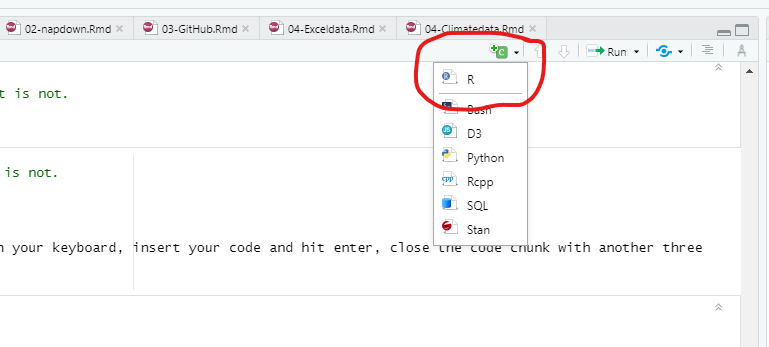
\includegraphics{tutorial_screenshots/code_chunk2.png}
\emph{Code chunks for other languages may be added from this list as well.}

\hypertarget{create-tables}{%
\subsection{Create tables}\label{create-tables}}

\hypertarget{option-1}{%
\subsubsection{Option 1}\label{option-1}}

Create table headers with dashed lines below the header title. Separate headers with tab or space between the headers and corresponding dashed lines.\\
Type in row values below the dashed lines. The row value length may exceed the dashed line length but MUST not extend into the next header's dashed line.\\
\textbf{Column alignment is based on the position of the header/column title relative to the dashed line below it.}\\
To insert a caption or alt text to your table use, full colon `:' followed by your caption text at the end of the table.\\
Alternatively, use `Table: your caption or text'. The following syntax (screenshot) produces the ensuing table.

\begin{figure}
\centering
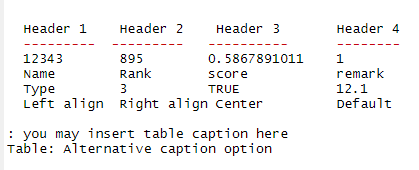
\includegraphics{tutorial_screenshots/typed_table.png}
\caption{manual table}
\end{figure}

\begin{longtable}[]{@{}lrcl@{}}
\caption{you may insert table caption here\\
Table: Alternative caption option}\tabularnewline
\toprule
Header 1 & Header 2 & Header 3 & Header 4 \\
\midrule
\endfirsthead
\toprule
Header 1 & Header 2 & Header 3 & Header 4 \\
\midrule
\endhead
12343 & 895 & 0.5867891011 & 1 \\
Name & Rank & score & remark \\
Type & 3 & TRUE & 12.1 \\
Left align & Right align & Center & Default \\
\bottomrule
\end{longtable}

\hypertarget{option-2}{%
\subsubsection{Option 2}\label{option-2}}

You may also create simple tables using a \texttt{knitr} function called \texttt{kable}.\\
The code below tells r that we want to create a data set with 3 columns, X, Y \& Z, assigning them the values enclosed in the letter c.~The letter c used together with brackets indicates a list of elements. Thus, in the example below, we tell r that our column X, will contain a list of 4 elements i.e 20, 30, 10 \& 50.\\
Then we tell r to create the data set by combining all the columns X, Y \& Z into a data frame.
Finally, we call the function \texttt{kable} and enter the data we created. This function converts our data frame into a table format.\\
Optionally, you may add a caption to the table and specify cell alignment.

\begin{figure}
\centering
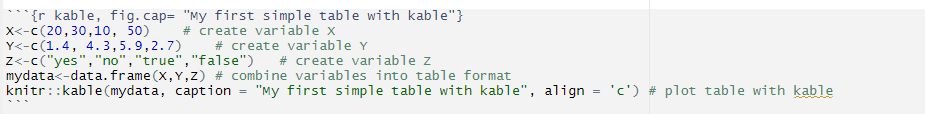
\includegraphics{tutorial_screenshots/kable_table.png}
\caption{kable table}
\end{figure}

\begin{table}[!h]

\caption{\label{tab:kable}My first simple table with kable}
\centering
\begin{tabular}[t]{c|c|c}
\hline
X & Y & Z\\
\hline
20 & 1.4 & yes\\
\hline
30 & 4.3 & no\\
\hline
10 & 5.9 & true\\
\hline
50 & 2.7 & false\\
\hline
\end{tabular}
\end{table}

\textbf{Note that our code chunk is labelled `kable'. You can label code chunks as below}

\begin{figure}
\centering
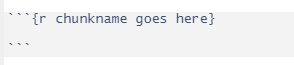
\includegraphics{tutorial_screenshots/chunk_name.png}
\caption{labled chunk}
\end{figure}

This will be useful for cross-referencing as we'll see in the \protect\hyperlink{chapter-references}{Chapter References} section.

\hypertarget{option-3}{%
\subsubsection{Option 3}\label{option-3}}

You may also generate tables using Microsoft excel data, using the \texttt{kable}package or a lot more other packages not covered in this release.
Please refer to chapter 5 \protect\hyperlink{working-excel-data}{Working Excel data} for details.

\hypertarget{page-breaks}{%
\subsection{Page breaks}\label{page-breaks}}

Use three or more asterisks or dashes to insert a page break.

\begin{figure}
\centering
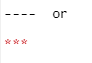
\includegraphics{tutorial_screenshots/page_break.png}
\caption{page break}
\end{figure}

\emph{Remember to add a blank line before the asterisks or dashes}

\hypertarget{process-a-markdown-document-to-desired-output}{%
\subsection{Process a markdown document to desired output}\label{process-a-markdown-document-to-desired-output}}

To create the desired output file document from the markdown format, use the function \texttt{render\ ("your\ .rmd\ file\ name)}.\\
Alternatively,and most commonly used, is the \texttt{Knit} button from the markdown script environment. The button is a blue ball of yarn around a crotchet, and is labeled `Knit'
When a document is rendered, rmarkdown saves the results/output file into your working directory, giving it the same name as your .rmd file, but with relevant extension (e.g.~as html if output type was set to html)

\begin{figure}
\centering
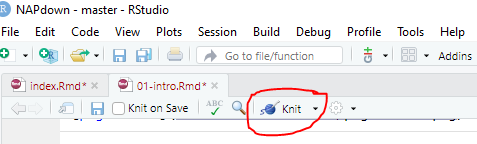
\includegraphics{tutorial_screenshots/knit_button.png}
\caption{knit}
\end{figure}

\hypertarget{references}{%
\subsection{References}\label{references}}

\hypertarget{citationsbibliography}{%
\subsubsection{Citations/Bibliography}\label{citationsbibliography}}

To add citations to our document, we need to add our reference document details to a text file saved in the .bib format e.g myrefences.bib. We also need to add this file to our bibliography parameter in the yaml section of the index.rmd file.\\
The references for this exercise are saved in the file `book.bib'.\\
To add your reference documents to the .bib file, use the BibTeX citation style i.e

\begin{figure}
\centering
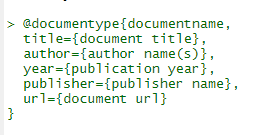
\includegraphics{tutorial_screenshots/citations.png}
\caption{citations}
\end{figure}

Sites such as \href{https://scholar.google.com/}{Google Scholar} have ready to use/ formatted bibliography styles such as BibTeX, EndNote etc. You may copy-paste the BibTeX text into your .bib file in r.

You may have as many documents listed in the .bib file but rmarkdown will only include those that have been referenced within your markdown document.\\
To reference documents in your narrative and thus, have them included in the reference section, use the format \texttt{{[}@documentname{]}}.\\
The references will appear at the end of the chapter where they are referenced, as well as in the overall `References' section.

\hypertarget{chapter-references}{%
\subsubsection{Chapter References}\label{chapter-references}}

To reference chapter, type in the chapter title inside square brackets. For instance, this command references our second chapter named NAPdown.

\begin{figure}
\centering

\includegraphics{tutorial_screenshots/ref_chapters_sections.png}
\caption{chapter ref}
\end{figure}

The same applies to section headers. Just type {[}section header name{]}.

\hypertarget{table-figure-references}{%
\subsubsection{Table \& Figure References}\label{table-figure-references}}

To reference figures use syntax `@ref(fig:code chunk label)' or'@ref(tab:code chunk label)' for tables.
For instance, we created our kable table in the code chunk named kable. To reference this table anywhere in our document, just type in command

\begin{figure}
\centering
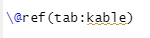
\includegraphics{tutorial_screenshots/ref_table.png}
\caption{Ref table}
\end{figure}

This will insert a reference link to the kable table.

\hypertarget{pandoc-knitr}{%
\subsection{Pandoc \& Knitr}\label{pandoc-knitr}}

\texttt{Pandoc} is a universal document converter designed to convert thousands of markup languages. So when we create our document in markdown and want to output it as a pdf, pandoc does the work.\\
\texttt{Knitr} on the other hand, is an r package that enables the integration of yaml, text and code evaluations into an output document. \texttt{Knitr} contains the \texttt{Knit} function through which we render our rmarkdown documents to our desired output format.
When you render a document in rmarkdown (or call the knit function), the rmarkdown document is converted to a basic markdown language (.md) which is then converted by pandoc to say html, pdf, word, etc as per user specifications.
\texttt{Knitr} and \texttt{pandoc} come in bundled with rmarkdown, and thus, there is no need to install them separately.\\
However, should you need to install pandoc as standalone, you may do so from the \href{http://pandoc.org}{Pandoc homepage}. In this regard, it is important to note that in as much as standalone installations may provide much higher versions of the software than what is already bundled in r, they are often not streamlined for use in r, and may thus cause some compatibility issues.

\hypertarget{napdown}{%
\chapter{NAPdown}\label{napdown}}

\hypertarget{setting-up-an-enap}{%
\section{Setting up an eNAP}\label{setting-up-an-enap}}

We will use the package \texttt{bookdown} to generate NAP document in a book format. Journal articles or reports can be produced in the same way.
We will also use the package \texttt{tinytex} to build pdf format of the book document.\\
1. First, launch the rstudio app in your pc.\\
2. Install the bookdown and tinytex packages in case you have not installed them. Use any of the methods shown in the \protect\hyperlink{installing-packages}{Installing packages} section.\\
3. Then from the menu bar go to \texttt{File-\textgreater{}\textgreater{}New\ Project-\textgreater{}\textgreater{}New\ Directory-\textgreater{}\textgreater{}Book\ Project\ using\ bookdown}.\\
A new window appears

\begin{figure}
\centering
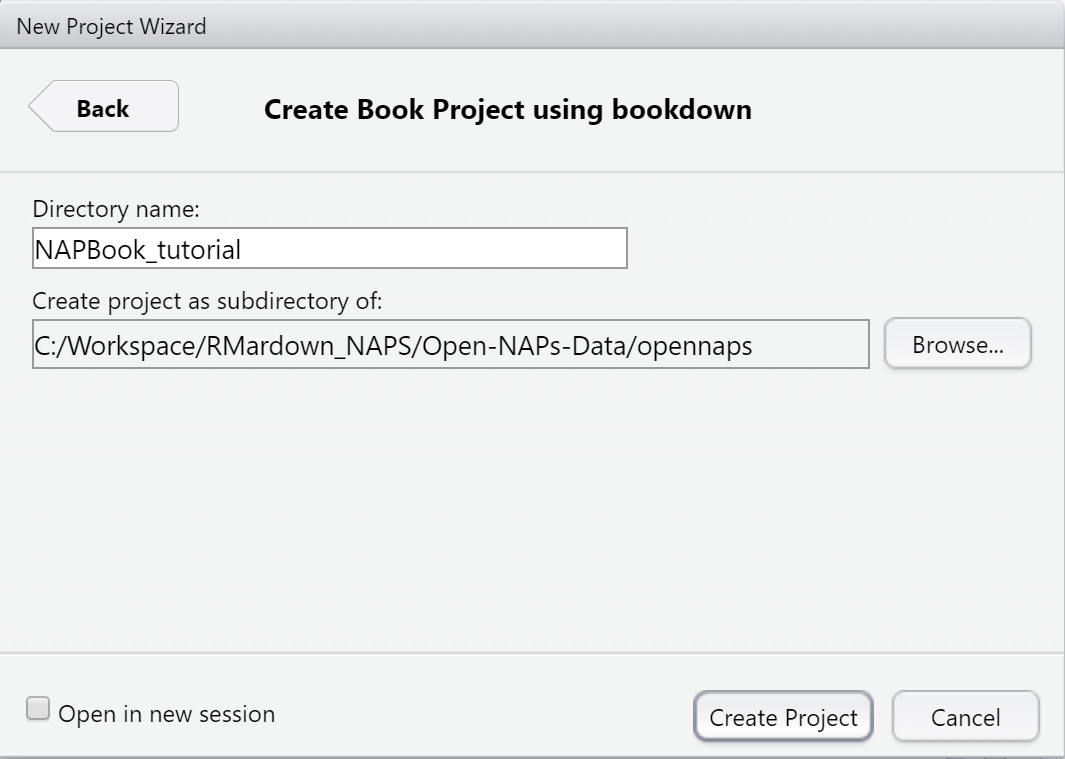
\includegraphics[width=4in,height=\textheight]{tutorial_screenshots/open_bkdown_proj.png}
\caption{Create Bookdown project\ldots{}}
\end{figure}

\begin{enumerate}
\def\labelenumi{\arabic{enumi}.}
\setcounter{enumi}{3}
\tightlist
\item
  Give your bookdown directory a name `NAPBook\_tutorial'. This is the name of a new folder that will be created to store your bookdwon project files.\\
\item
  In the `Create project as subdirectory of' field, use the browse button to navigate to where you want to save your bookdown project folder.\\
\item
  After you select the directory location, you are returned to the `Create Book project\ldots{}' window. Click `create project'.\\
  A new project session opens up, with skeleton chapters and other sections and metadata files.\\
  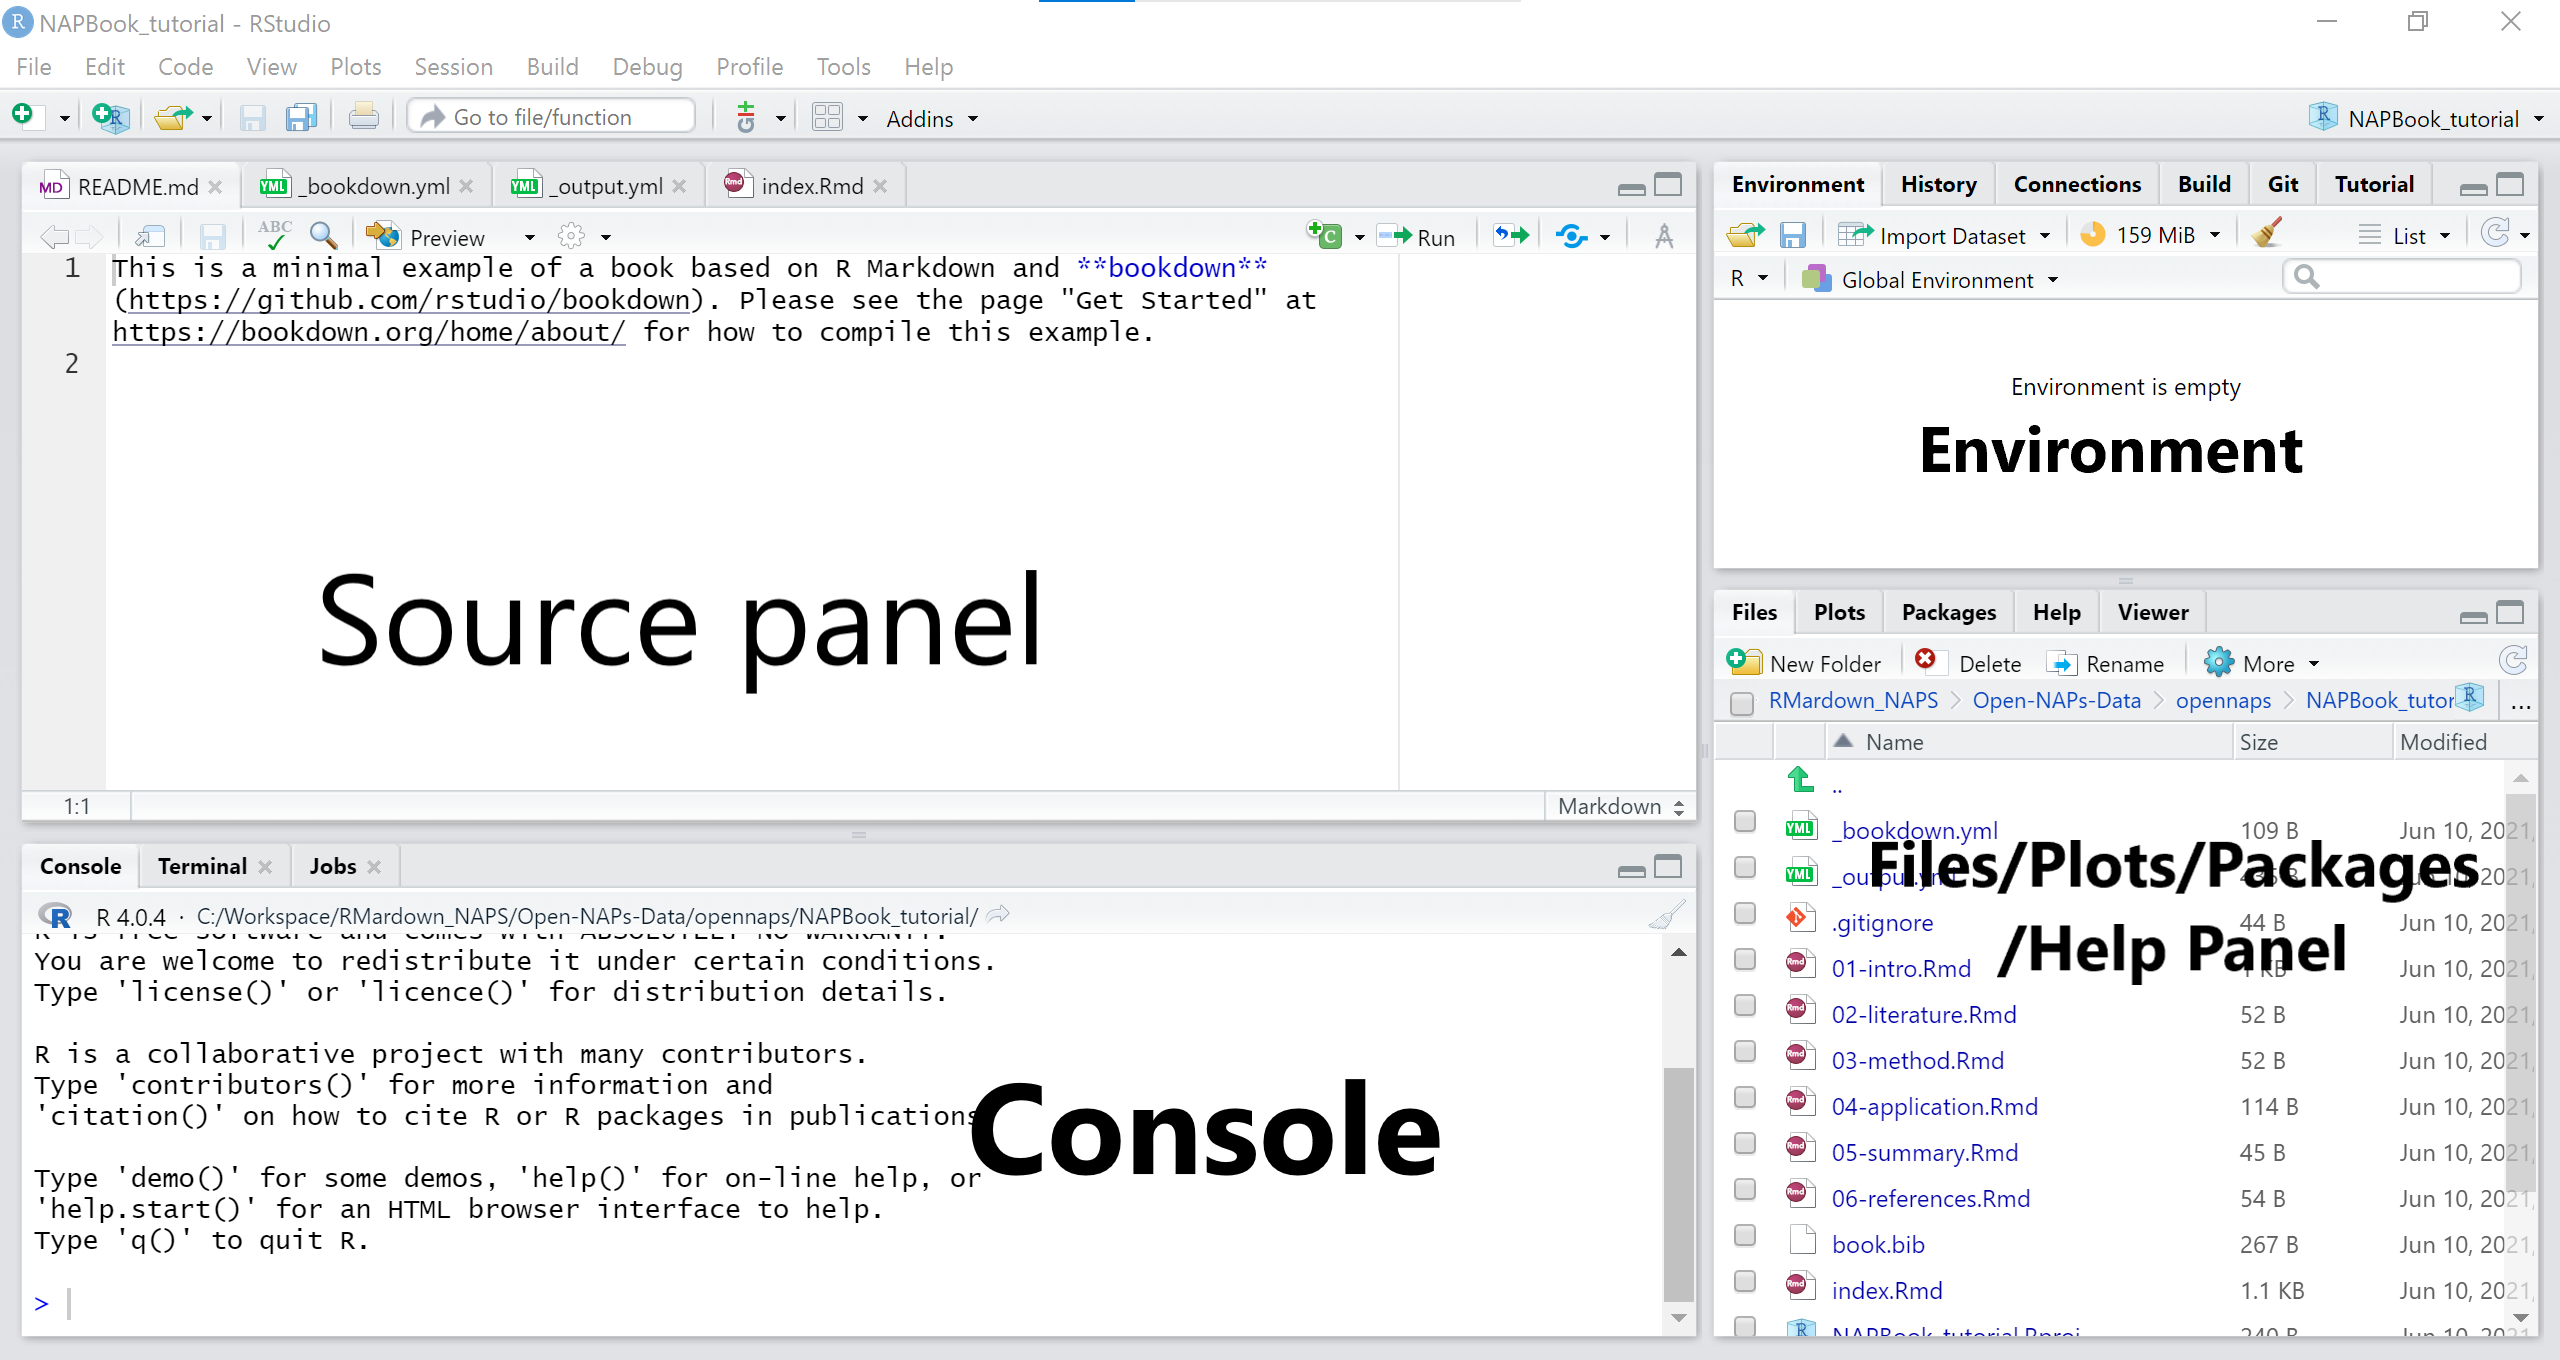
\includegraphics{tutorial_screenshots/bkdn_proj_window_label.png}\\
  Your project window might appear with panel arrangements different from mine/in screenshot. Your project files can be accessed from the Files tab in bottom right of the project window.
\end{enumerate}

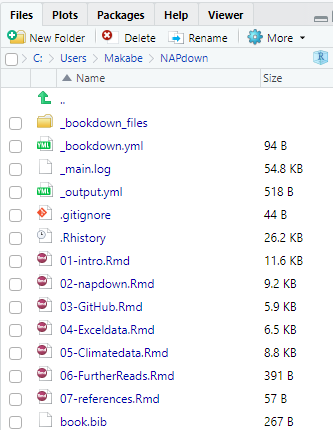
\includegraphics{tutorial_screenshots/files_panel.png}
Each chapter is compiled from a single .rmd file, and always starts with a first level header sign `\#'.\\
From the files pane, you can open any chapter, and edit it to your liking.

Lets take a look at the '\_bookdown.yml' file.

\begin{enumerate}
\def\labelenumi{\arabic{enumi}.}
\setcounter{enumi}{6}
\tightlist
\item
  From the `Files' tab, click on the \_bookdown.yml' file.\\
  The file opens up in your script/source pane. Notice, the book\_filename takes the name of the folder we created when opening the project.\\
\item
  Let's add the line \texttt{output\_dir:\ "docs"} to this file.
  See screenshot below;
\end{enumerate}

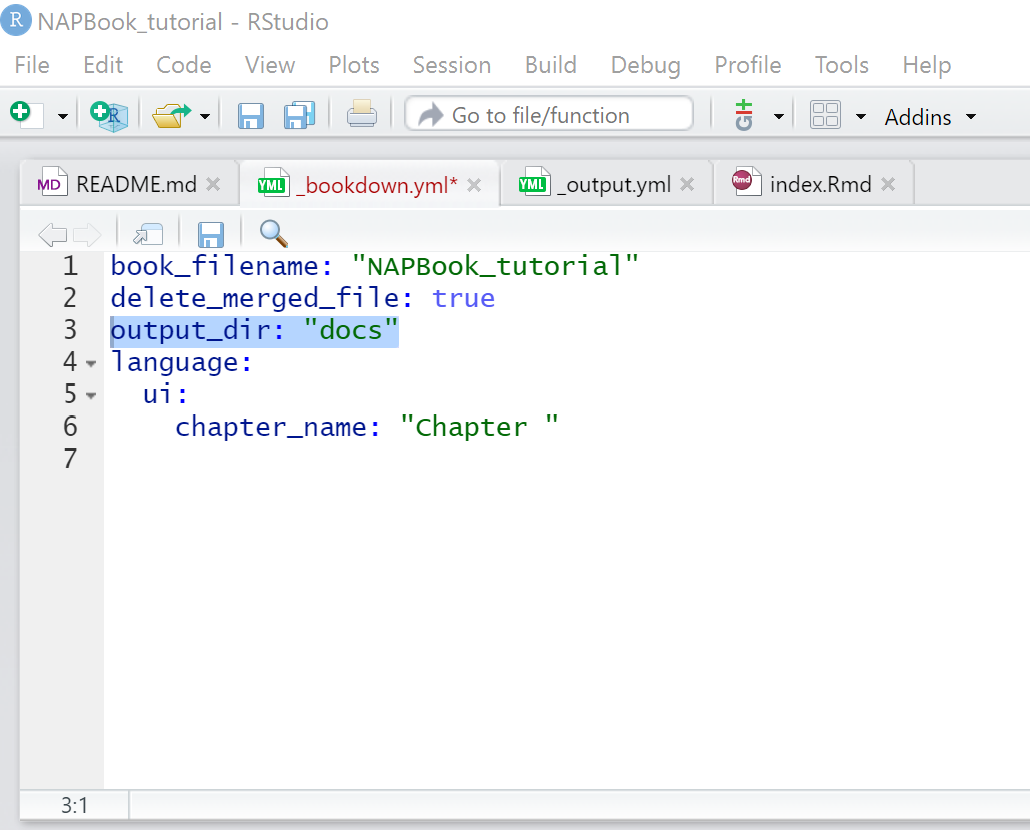
\includegraphics{tutorial_screenshots/add_docs_to_bkdnyaml.png}\\
This command creates an additional folder called `docs' and specifies that we want to store our outputs here. This folder is necessary for creating webpages from our book project.\\
9. Save changes. Use the `Save' icon on the script window or Ctrl + S on your keyboard.\\
10. Next, click to open the '\_output.yml' file.\\
11. Let's edit the line that contains the title to our book. Change the text `A Minimal Book \ldots{}' to `NAP Book Tutorial'.\\
Should look like this;

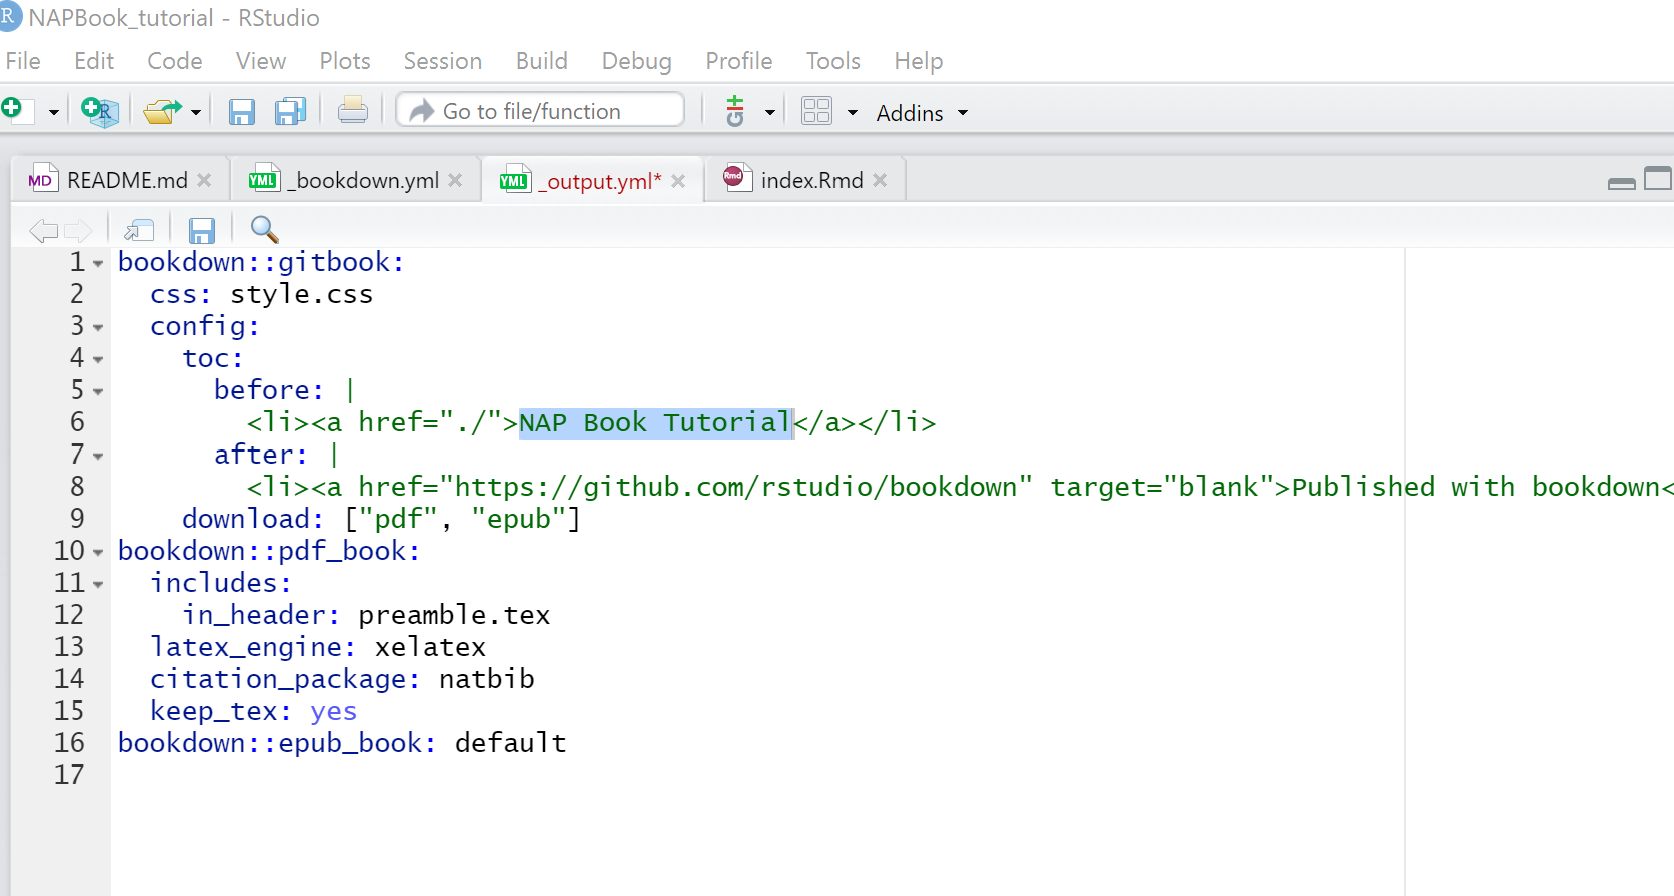
\includegraphics{tutorial_screenshots/edit_title_output_yaml.png}\\
Ignore everything else for now :)\\
12. Save.\\
13. Scroll down your files to find the `index.rmd' file. Click to open.\\
14. Edit the title, author \& description fields in the yaml header section.\\
15. Delete all text, except the last code chunk.\\
16. Add a chapter named `Preliminaries' before the code chunk.\\
Chapters are created using the first level header \#.\\
17. Add sections to your chapter using second level header \#\#.\\
Your script should look more or less similar to this;

\begin{figure}
\centering
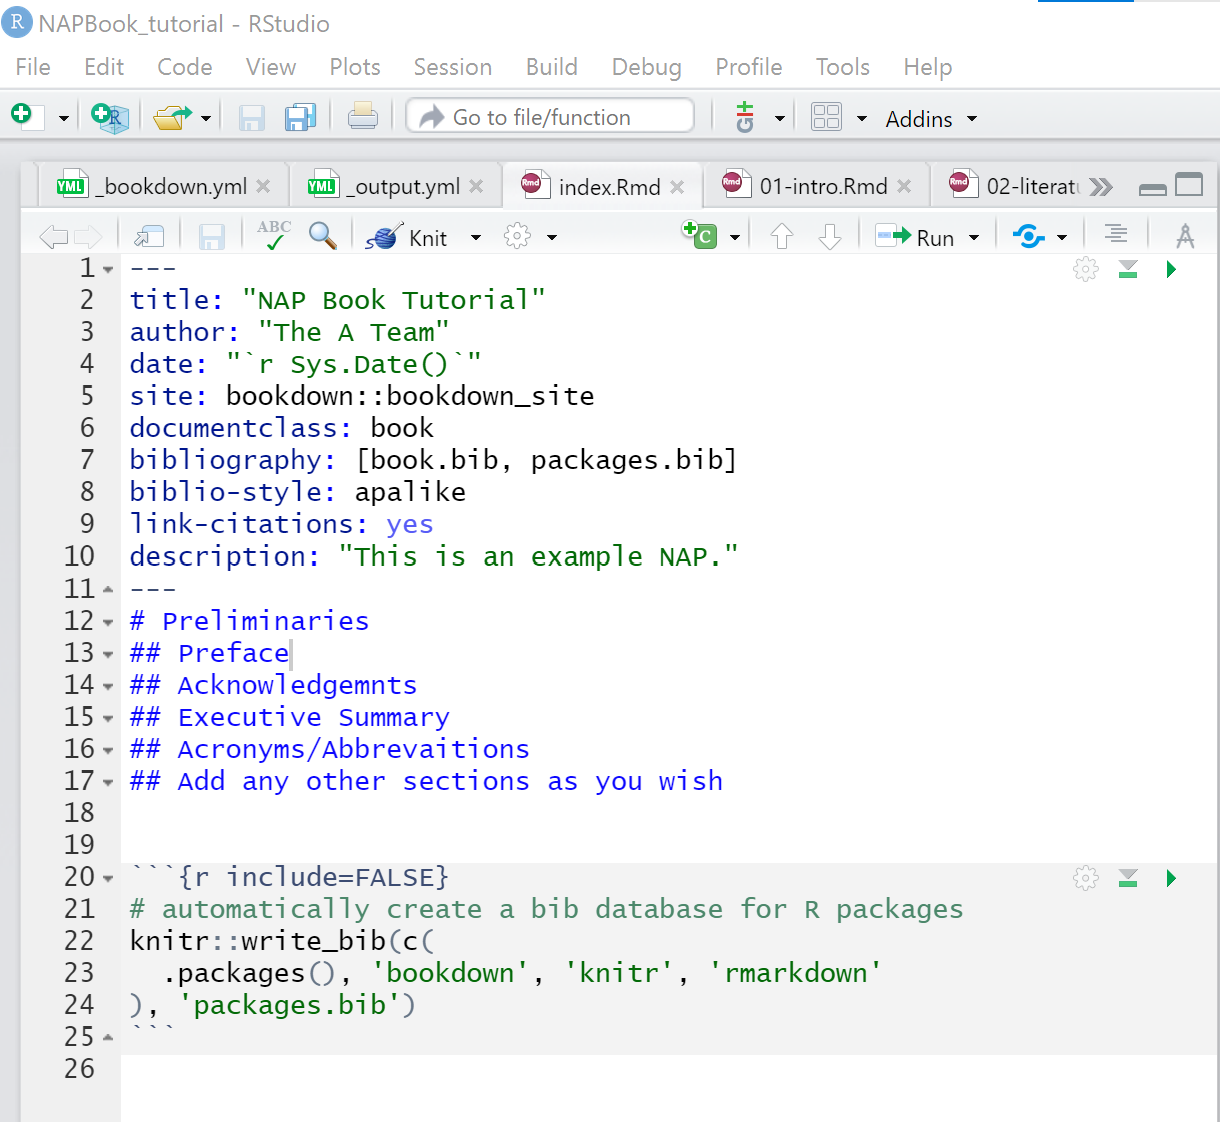
\includegraphics{tutorial_screenshots/edit_index.png}
\caption{edit book title and author}
\end{figure}

\begin{enumerate}
\def\labelenumi{\arabic{enumi}.}
\setcounter{enumi}{17}
\tightlist
\item
  Next, open the `README.md' file and edit the text to this `This is an example NAP designed to help you get started with creating your NAPs with bookdown.'. Or add a description of your choice.
\item
  Save your work.\\
\item
  Open the `01-Intro.rmd' file.\\
\item
  Type in the chapter title `Introduction'\\
\item
  Type in sub-chapters with the names `Overview of the NAP Process, NAP Vision, NAP Mandate, NAP Process in Sierra Leone, Functions, Guiding Principles, Goals, Overview of the NAP'\\
  Your script should resemble this;
\end{enumerate}

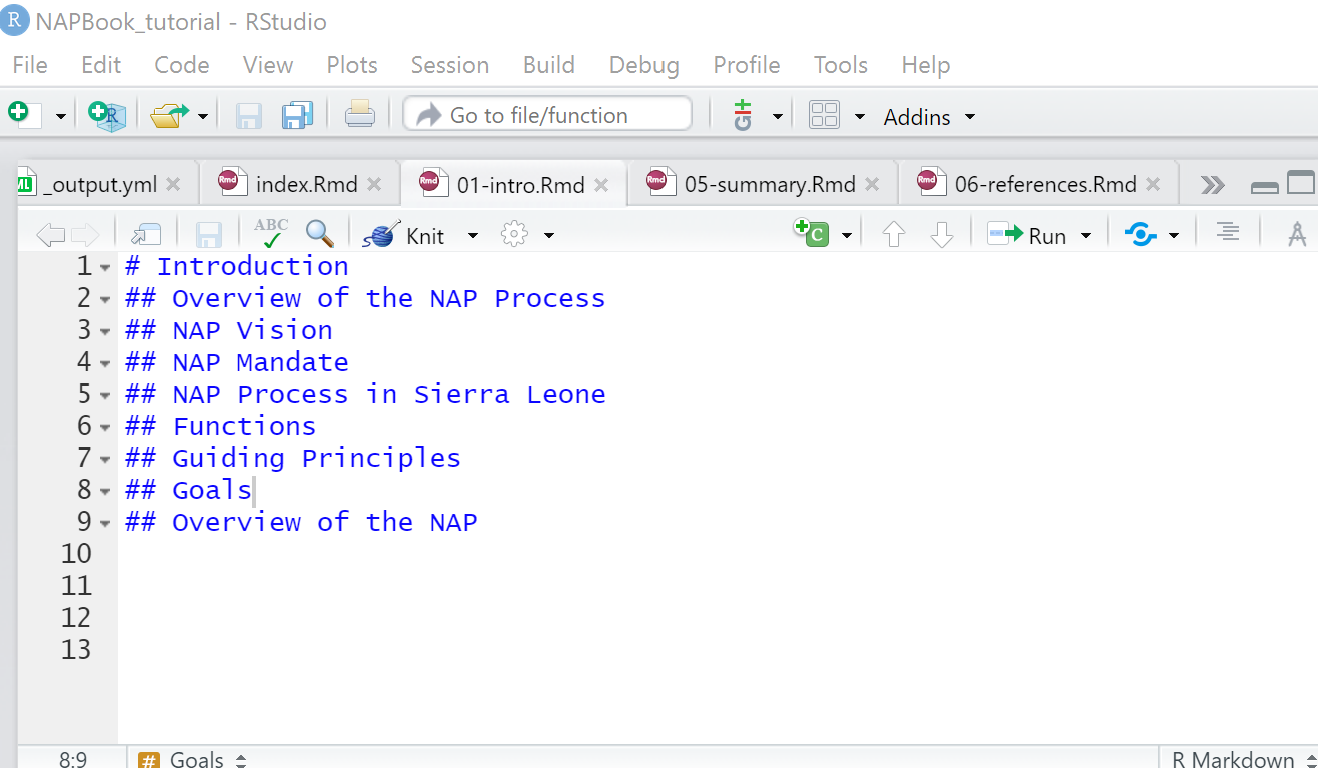
\includegraphics{tutorial_screenshots/intro_chapter.png}\\
This text has been borrowed from the Sierra Leone NAP. Use the text from the screenshot below to edit the next two chapters (.rmd files). i.e `02-literature.rmd \& 03-methods.rmd'.\\
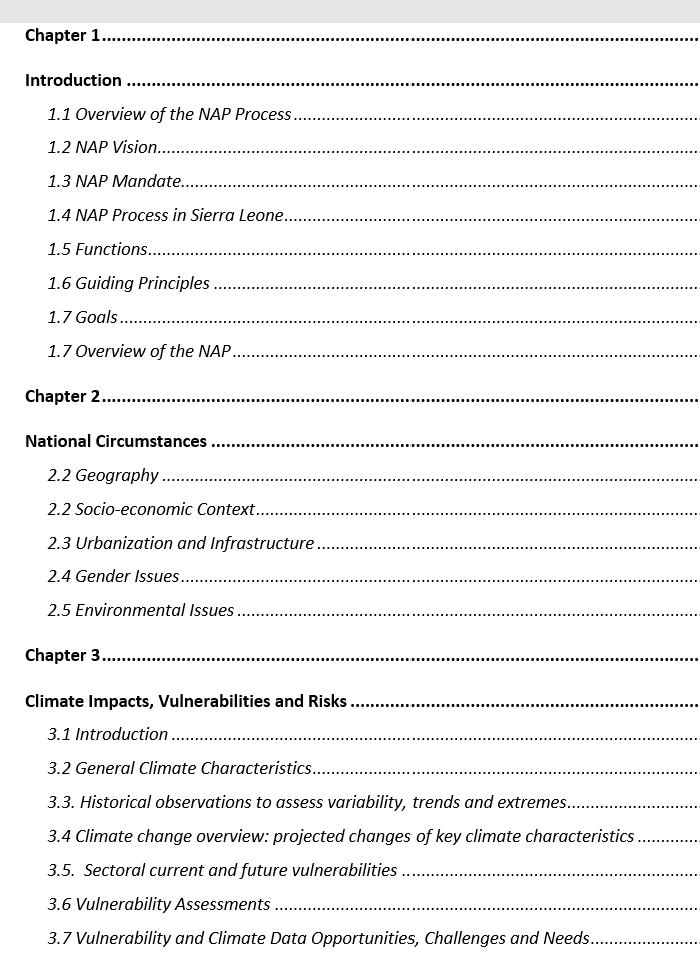
\includegraphics{tutorial_screenshots/SLeone_NAP_chapters.png}\\
For the interest of time, let's delete chapters 4 and 5 from our project files.\\
23. From the files tab (bottom right), click on the check-boxes to the left of the application and summary .rmd files to select them.
24. Click delete

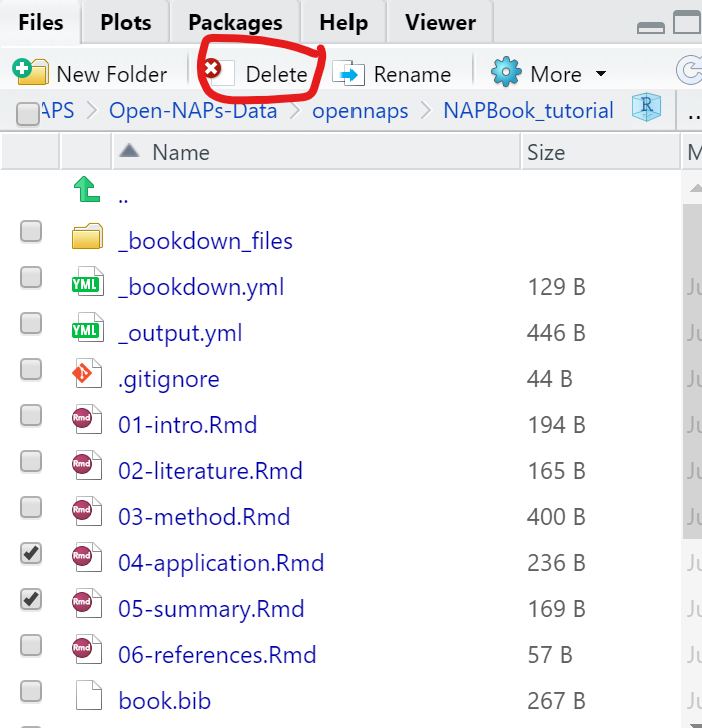
\includegraphics{tutorial_screenshots/delete_4_5.png}
25. Save project.\\
26. From the `Environment' window, click on the tab `Build'.\\
27. On the new window that opens, click the hammer/Build Book button to start rendering the book.

\begin{figure}
\centering
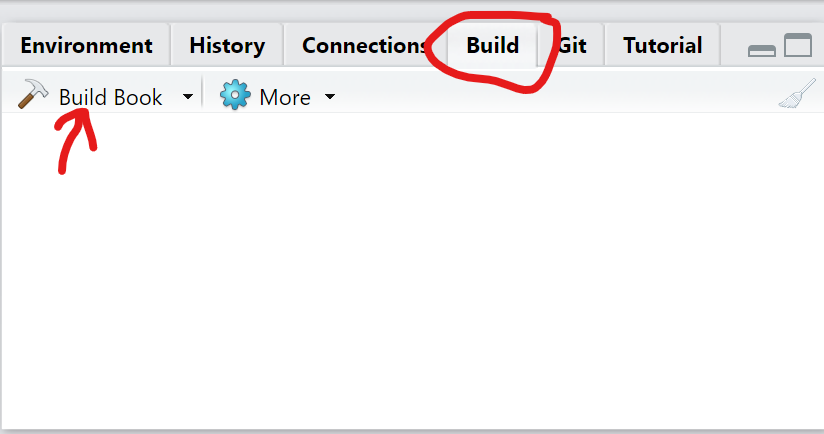
\includegraphics{tutorial_screenshots/build_book.png}
\caption{Build book}
\end{figure}

This process may take a few minutes. You can monitor the progress in the Environment window.\\
When the process is done, your book should open up in an html window as below;\\
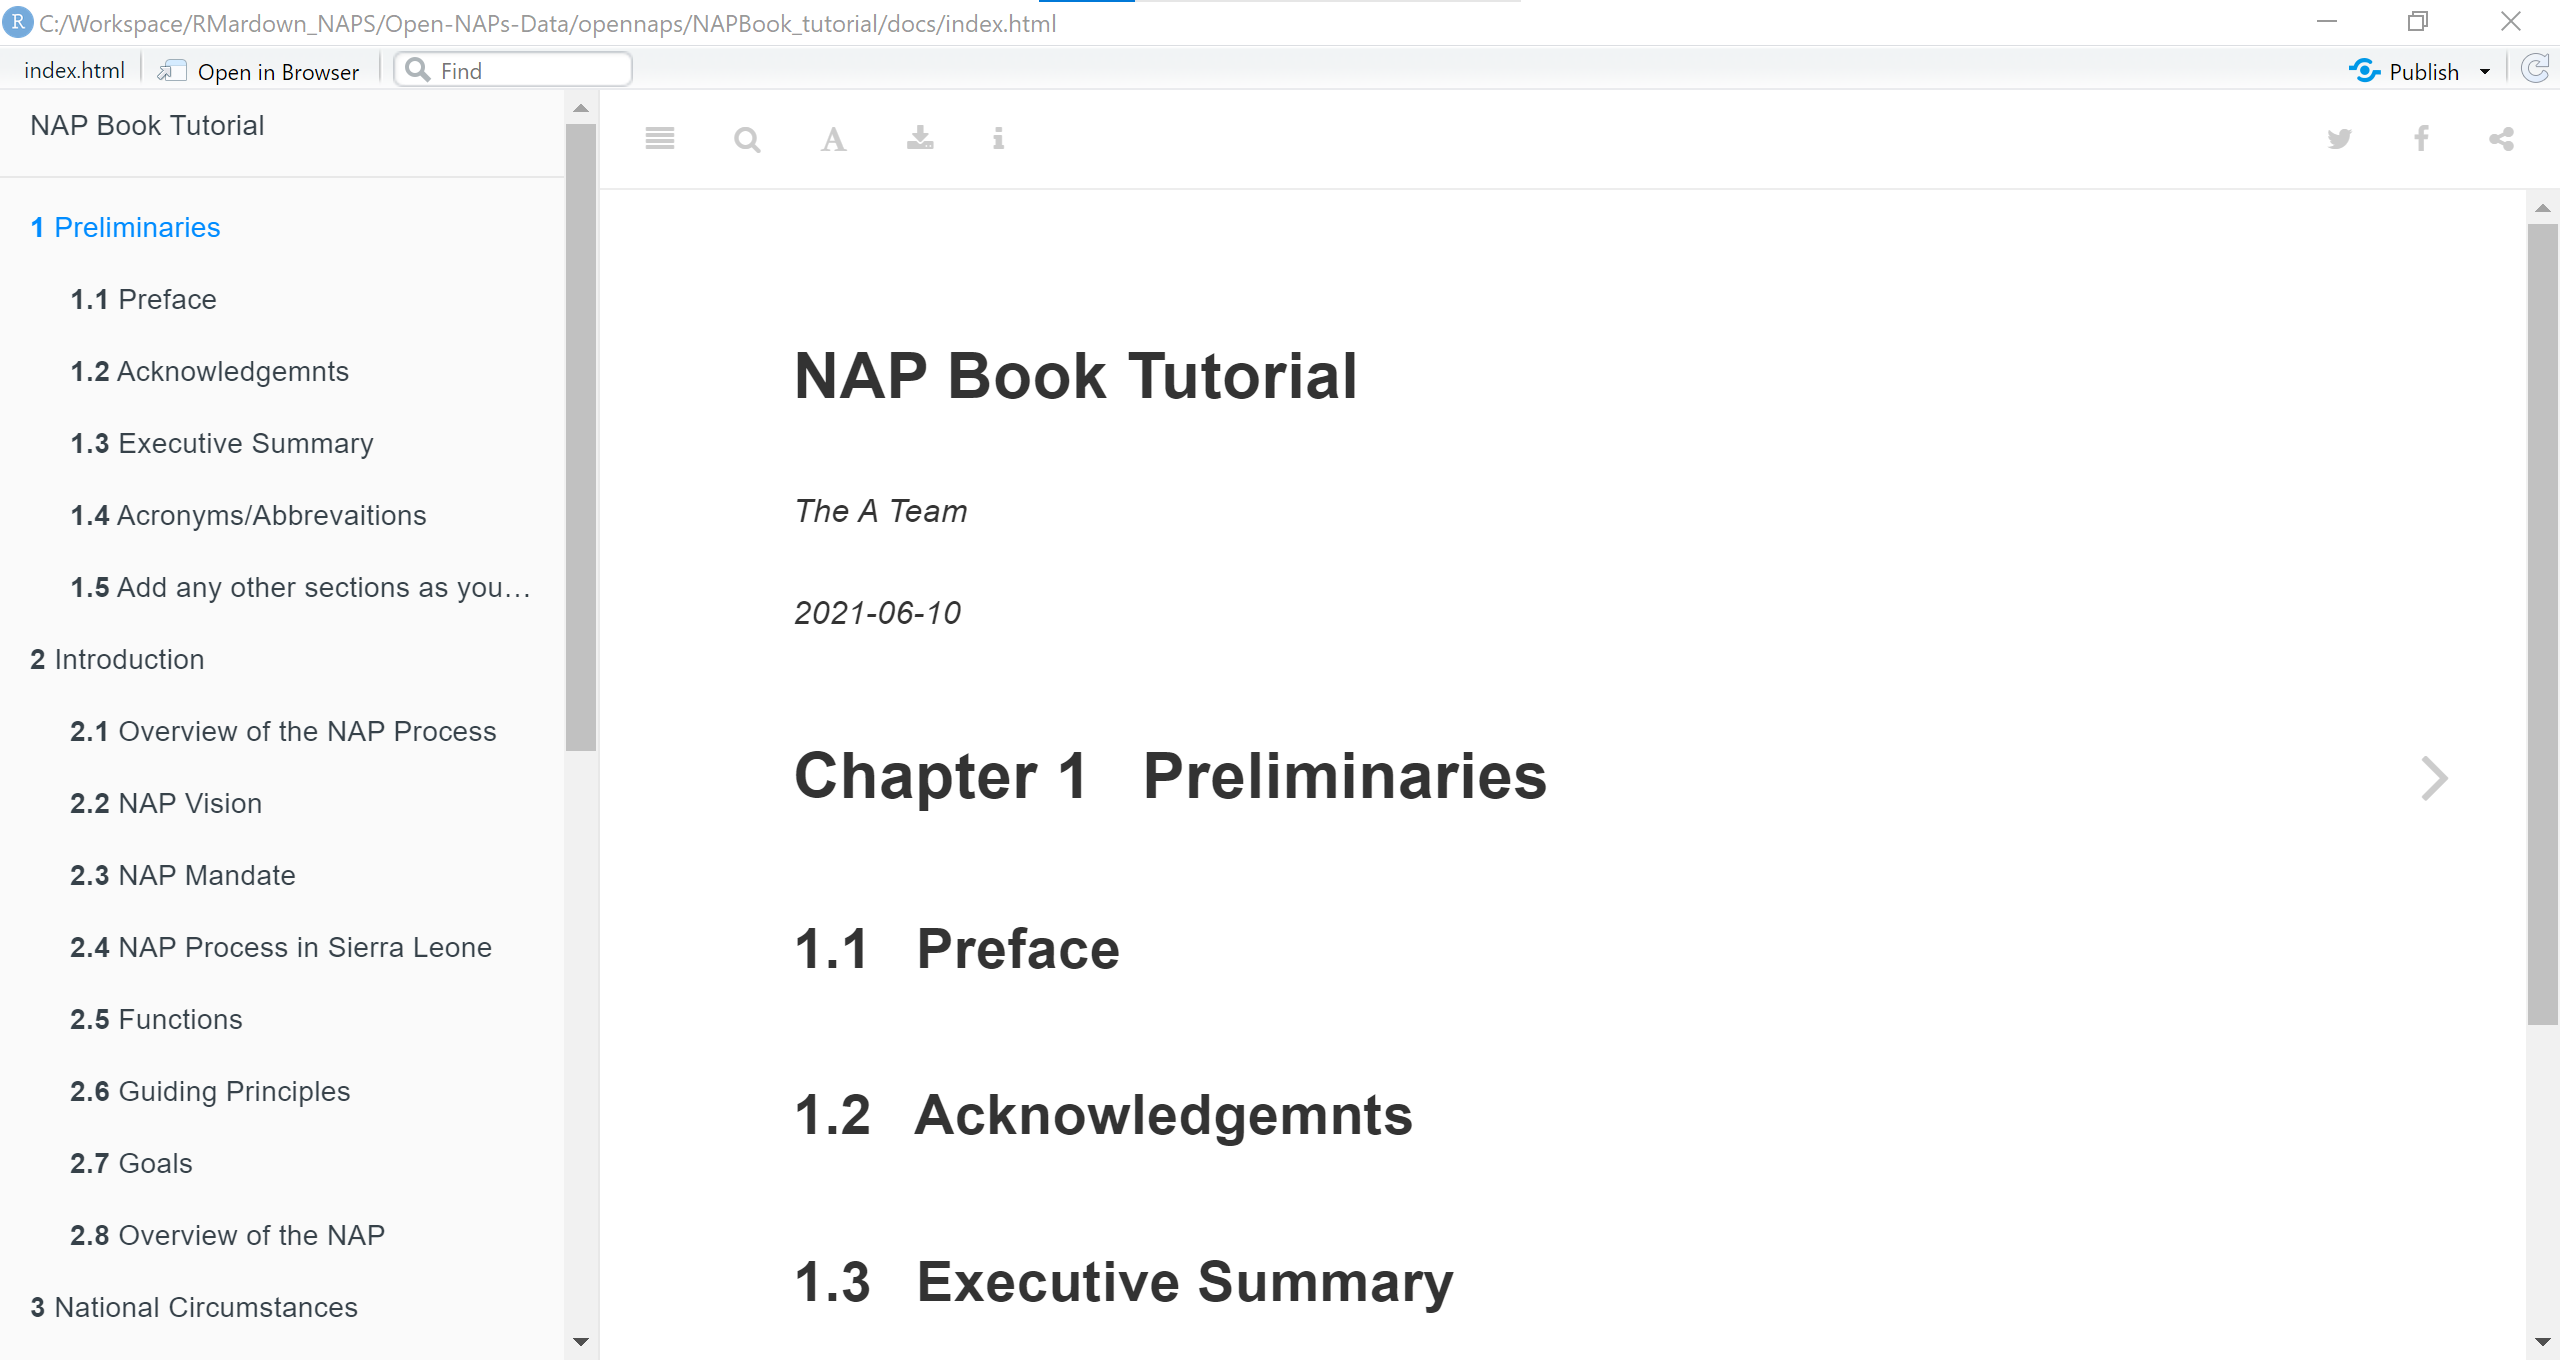
\includegraphics{tutorial_screenshots/built_book.png}\\
28. Scroll down your chapters to find the `References' chapter. Oops! No reference! Don't sweat.\\
29. Back to our project, from the Files tab in bottom right window, open the file named `book.bib'. This is the text file holding our citations.Currently, only one. You will notice that the document type is a book, and the the book name is `xie2015'.

\includegraphics{tutorial_screenshots/add_citation.png}
30. To cite this book in our NAP book, open square brackets and type the `@' sign followed by the book name. i.e \citep{xie2015}.\\
31. Let's use this citation say in the Introduction chapter. Open the chapter, and insert the text `Our only citation at the moment is \citep{xie2015}'. See example:\\
\includegraphics{tutorial_screenshots/cite_book.png}
32. Run the `Build Book' command again.\\
33. Now you should see that your book has been added to the `References' section, both in the chapter in which you cited it as well as in the overall References Chapter.

\begin{figure}
\centering
\includegraphics{tutorial_screenshots/reference_incl.png}
\caption{citation added to ref}
\end{figure}

\textbf{Congratulations!!!}

\hypertarget{integrating-code-evaluations-within-your-text-chapters}{%
\section{Integrating code evaluations within your text/ chapters}\label{integrating-code-evaluations-within-your-text-chapters}}

To integrate a code (+ its evaluation), open a code chunk at your desired section or paragraph and write your code as below. Please refer to the section on \protect\hyperlink{insert-code-chunks}{Insert code chunks} if need be.

For instance in the code below we use one of the in-built R datasets named \texttt{mtcars} to plot a bar chart of Car `Model' against `mpg' (miles per gallon).
When this code is evaluated, the bar chart will be plotted within your document as specified. You may enter text before or after the plot.

\begin{Shaded}
\begin{Highlighting}[]
\FunctionTok{library}\NormalTok{(plotly)}
\NormalTok{plotly}\SpecialCharTok{::}\FunctionTok{plot\_ly}\NormalTok{(mtcars,}\AttributeTok{type =} \StringTok{\textquotesingle{}bar\textquotesingle{}}\NormalTok{, }
                \AttributeTok{x=}\FunctionTok{row.names}\NormalTok{(mtcars), }\AttributeTok{y=}\SpecialCharTok{\textasciitilde{}}\NormalTok{mpg)}\SpecialCharTok{\%\textgreater{}\%}
\NormalTok{  plotly}\SpecialCharTok{::}\FunctionTok{layout}\NormalTok{(}\AttributeTok{yaxis=}\FunctionTok{list}\NormalTok{(}\AttributeTok{tickfont=}\FunctionTok{list}\NormalTok{(}\AttributeTok{size=}\DecValTok{10}\NormalTok{)),}
                 \AttributeTok{xaxis=}\FunctionTok{list}\NormalTok{(}\AttributeTok{tickfont=}\FunctionTok{list}\NormalTok{(}\AttributeTok{size=}\DecValTok{10}\NormalTok{)))}
\end{Highlighting}
\end{Shaded}

\includegraphics{_main_files/figure-latex/unnamed-chunk-2-1.pdf}

Below is another example using precipitation data from worldclim

\begin{Shaded}
\begin{Highlighting}[]
\FunctionTok{library}\NormalTok{(raster) }\CommentTok{\# library responsible for plotting the data}

\NormalTok{pr}\OtherTok{\textless{}{-}}\FunctionTok{getData}\NormalTok{(}\StringTok{"worldclim"}\NormalTok{, }\AttributeTok{var=}\StringTok{\textquotesingle{}prec\textquotesingle{}}\NormalTok{, }\AttributeTok{res=}\DecValTok{5}\NormalTok{) }\CommentTok{\# reading/accessing the data}

\FunctionTok{plot}\NormalTok{(pr}\SpecialCharTok{$}\NormalTok{prec1) }\CommentTok{\# plot the first layer of the data (precipitation for the month of January)}
\end{Highlighting}
\end{Shaded}

\includegraphics{_main_files/figure-latex/unnamed-chunk-3-1.pdf}

\hypertarget{some-things-to-note}{%
\subsection{Some things to note}\label{some-things-to-note}}

\begin{enumerate}
\def\labelenumi{\arabic{enumi}.}
\tightlist
\item
  To create additional chapters, create a new /empty .rmd file and save it under your bookdown directory. Use the same numbering structure as the default chapters (i.e.~01,02,03, etc).\\
  We will learn about advanced numbering and re-ordering chapters later.\\
\item
  Use the \texttt{knit} function to render and preview a single chapter.\\
\item
  From our output.yml file, you will notice that we have 3 output options for our file; gitbook, pdf and epub. This is the default. You may select the most preferred output type by deleting the other/unwanted formats or leave this as default and choose a single output format when building the book. Since we left the default 3 options, when we rendered the book, it was compiled in .tex/gitbook, pdf and epub. This can be accessed from the `docs' folder.
\end{enumerate}

\includegraphics{tutorial_screenshots/docs_folder_contents.png}\\
4. When building the book. Here you may choose to build one or all formats. From the Build Book button, click on the drop-down arrow and select your preferred format.

\begin{figure}
\centering
\includegraphics{tutorial_screenshots/build_book_drop_down.png}
\caption{Build book format options}
\end{figure}

\hypertarget{some-troubleshooting}{%
\section{Some Troubleshooting}\label{some-troubleshooting}}

Creating pdf documents using LaTeX engines and distributions such as TinyTeX is not a straightforward task and may produce errors as the process involves multiple processing activities. However, most errors can be solved using suggestions contained in the error messages produced in the Environment or Console windows.\\
If, in any case, the LaTeX error generated is not clear, you may use any the commands options below to solve the problem.

\emph{Remove the \# sign to run code}

\begin{Shaded}
\begin{Highlighting}[]
\CommentTok{\# remotes::install\_github(\textquotesingle{}yihui/tinytex\textquotesingle{}) \#\#install the development version of tinytex}

\CommentTok{\# update.packages(ask = FALSE, checkBuilt = TRUE) \#\# update your r and}
\CommentTok{\# tinytex::tlmgr\_update() \#\# tinytex packages}

\CommentTok{\# tinytex::reinstall\_tinytex()  \#\# 3 reinstall tinytex}

\CommentTok{\# options(tinytex.verbose = TRUE) \#\# 4 set this option in an r code chunk.This helps provide more info on your problems. Remember to remove it after solving your problem}
\end{Highlighting}
\end{Shaded}

See more on \href{https://yihui.org/tinytex/r/}{TinyTex Debugging}.

Additionally, quite often, LaTeX formatting is not very compatible with other output formats such as html. But with the use of \texttt{html\ widgets} and other advanced formatting options, this problem can be overcome.
To produce a pdf document from a document with both LaTeX and html formats, it may be useful to install the package \texttt{webshot} from CRAN.

\begin{Shaded}
\begin{Highlighting}[]
\CommentTok{\#install.packages("webshot")  }
\CommentTok{\# webshot::install\_phantomjs() }
\end{Highlighting}
\end{Shaded}

Further reading on \href{https://bookdown.org/yihui/bookdown/html-widgets.html}{html widgets here}

\hypertarget{github-github-pages}{%
\chapter{GitHub \& GitHub Pages}\label{github-github-pages}}

Github is great for project collaboration, backup and version control.
To use github as your repository manager, Create an account at (\url{https://github.com/})
You may additionally download and install the desktop version \href{https://desktop.github.com/}{here}

\hypertarget{sharing-repositories-on-github}{%
\section{Sharing Repositories on GitHub}\label{sharing-repositories-on-github}}

\hypertarget{via-github-desktop}{%
\subsection{Via GitHub Desktop}\label{via-github-desktop}}

To use this option, download and install the gh desktop version \href{https://desktop.github.com/}{here}

\begin{enumerate}
\def\labelenumi{\arabic{enumi}.}
\item
  Open GitHub desktop on your pc/laptop\\
\item
  On the main menu, click on \texttt{File} and select \texttt{Add\ local\ repository} from the dropdown list\\
  \includegraphics{tutorial_screenshots/gh_desktop_add_repo.png}\\
\item
  Browse to your your repository is sitting in your pc, select it and click `Add Repository'
\item
  A list of all your files and sub-directories appears from which you may select and deselect what you want to publish to GitHub.
\item
  Enter a commit message on the `Summary' text-box right below your listed files and optionally a brief description.\\
  \includegraphics{tutorial_screenshots/gh_desktop_commit.png}\\
\item
  Hit `Commit to master'
\item
  To the right of the GitHub desktop window, the app will notify you that this repository is only available on your local machine and if you would like to share/publish it to GitHub. Click on publish repository\\
  \includegraphics{tutorial_screenshots/gh_desktop_publish_repo.png}\\
\item
  Uncheck the box for `keep the code private' and Click \texttt{Publish\ repository}\\
  \includegraphics{tutorial_screenshots/gh_desktop_uncheck_private.png}
\item
  From the menu bar on GitHub desktop, click on \texttt{Repository} and select \texttt{Push} from the drop-down list.
\item
  Congratulations, you just published your repository to GitHub
\end{enumerate}

\hypertarget{via-direct-file-upload}{%
\subsection{Via direct file upload}\label{via-direct-file-upload}}

\begin{enumerate}
\def\labelenumi{\arabic{enumi}.}
\tightlist
\item
  Log in to your GitHub.com account
\item
  Click on the plus sign + located at the top right corner of your github account page.
\end{enumerate}

\includegraphics{tutorial_screenshots/gh_create_repo.png}\\
3. Click on `New Repository' from the drop-down menu.\\
4. On the new window that appears, give the repository a name: NAPBook\_Tutorial\\
5. Leave the repository as `Public'
6. Leave everything else as is\\
7. Scroll down and click on `Create Repository'\\
8. On the resulting window, click on `upload an existing file'

\begin{figure}
\centering
\includegraphics{tutorial_screenshots/gh_uploadfiles.png}
\caption{import repo to github}
\end{figure}

This will take you to a new window, from which you can drag-\&-drop or browse to your files.

\begin{enumerate}
\def\labelenumi{\arabic{enumi}.}
\setcounter{enumi}{8}
\tightlist
\item
  Click on `choose your files'.\\
\item
  Navigate with the file explorer to where we saved our `NAPBook\_tutorial' folder in your pc.\\
\item
  Select everything within this folder, and click `Open'.\\
  Your files will start loading. Give it a minute or so.\\
  If you scroll through the files you will notice that our `docs' folder is missing. Do not worry!\\
\item
  To add the folder, lets use the drag and drop method. From your file explorer, navigate to our NAPBook\_tutorial folder, and click once on the `docs' folder to select it.\\
\item
  Drag and drop this folder into your github repository. The files should start uploading.\\
\item
  After your files finish uploading, scroll down to the `Commit changes' field; here you may enter a short description for your files. Let's enter the text `our first NAP book commit'\\
  When making changes to your files, you may use this field to briefly describe what changes you made, otherwise commonly known as commits.\\
\item
  Next, hit the `Commit changes' button at the end. This is called commiting.
\end{enumerate}

\hypertarget{via-git-bash}{%
\subsection{Via Git Bash}\label{via-git-bash}}

\begin{enumerate}
\def\labelenumi{\arabic{enumi}.}
\tightlist
\item
  Download and install Git Bash from this link (\url{https://git-scm.com/downloads}).\\
\item
  Repeat steps 1 - 7 in the preceding section.\\
\item
  On the new window, click on the `https' tab to reveal the url for your repository.
\end{enumerate}

\begin{figure}
\centering
\includegraphics{tutorial_screenshots/gh_repolink.png}
\caption{Repository url}
\end{figure}

\begin{enumerate}
\def\labelenumi{\arabic{enumi}.}
\setcounter{enumi}{3}
\tightlist
\item
  Luanch Git Bash on your pc. This opens up a window with your pc name in the text. This is the command window.\\
\item
  Set the working repository to where your project files are located. To do this, type in commamd \texttt{cd\ "path\ to\ your\ project\ files\ directory}. Click Enter on your keyboard.\\
\item
  Type in \texttt{git\ init} to initialize this directory as your file origin.\\
\item
  Type in \texttt{git\ remote\ add\ origin} the paste the https link from step 4. Click Enter.\\
\item
  Type in \texttt{git\ add\ .} to add all project files in your pc to your github repository.\\
\item
  To add only specific file, type in \texttt{git\ add\ .insert\ name\ of\ file}\\
\item
  Type in \texttt{git\ commit\ -m}, open quotation marks and insert a commit message. Click Enter.\\
\item
  Type in \texttt{git\ push\ origin\ master} and click Enter. This pushes/uploads your files plus the commit message to your github repo.\\
  Below is a list of the above commands
\end{enumerate}

\begin{figure}
\centering
\includegraphics{tutorial_screenshots/gh_bash_upload.png}
\caption{Upload files via git bash}
\end{figure}

\textbf{Congratulation once again!}

To share your repository with colleagues and friends, just copy the link on your browser and share it with them. The link should take a similar identity as below;

\begin{quote}
\url{https://github.com/yourusername/NAPBook_Tutorial}
\end{quote}

\hypertarget{publishing-to-github-pages}{%
\section{Publishing to GitHub pages}\label{publishing-to-github-pages}}

Github pages helps you to create/publish websites in very simple steps.
We will publish the NAP book we just created with bookdown into a git-based website.
To do this,\\
1.In your github repository, click on the \texttt{Settings} tab (right side of your screen)\\
2. Scroll down the listed menu items on the left side of the screen until you find menu item \texttt{Pages}. Click on it.

\includegraphics{tutorial_screenshots/gh_pages_setup.png}\\
3. Scroll down to the `Source' field. Click on the drop-down arrow and select the \textbf{main/master} branch and \textbf{docs} folder as your source files for your website. Click Save.\\
A message with a link to your website will appear, right above the \texttt{Source} field.

\begin{quote}
Your site is ready to be published at \url{https://yourusername.github.io/repositoryname/}
\end{quote}

or as seen here:
\includegraphics{tutorial_screenshots/gh_pageslink.png}

Use this link to view your newly created website.\\
4. Alternatively, navigate back to your main repository area, scroll down to your right to find your active \texttt{github-pages}. Click to view your website deployments.

\begin{figure}
\centering
\includegraphics{tutorial_screenshots/gh_pages_deploy.png}
\caption{gh pages deployment}
\end{figure}

\textbf{Now give yourself a pat on the back!}

\hypertarget{working-excel-data}{%
\chapter{Working Excel data}\label{working-excel-data}}

\hypertarget{prep}{%
\section{Prep}\label{prep}}

Steps;

\hypertarget{install-packages}{%
\subsection{Install packages}\label{install-packages}}

\begin{Shaded}
\begin{Highlighting}[]
\CommentTok{\#install.packages(c("readxl", "magrittr", "knitr", "kableExtra", "DT", "plotly", "dplyr", "ggplot2", "treemapify"))}
\end{Highlighting}
\end{Shaded}

\hypertarget{call-libraries-for-the-installed-packages}{%
\subsection{Call libraries for the installed packages}\label{call-libraries-for-the-installed-packages}}

\begin{Shaded}
\begin{Highlighting}[]
\FunctionTok{library}\NormalTok{(readxl)}
\FunctionTok{library}\NormalTok{(magrittr)}
\FunctionTok{library}\NormalTok{(knitr)}
\FunctionTok{library}\NormalTok{(kableExtra)}
\FunctionTok{library}\NormalTok{(DT)}
\FunctionTok{library}\NormalTok{(plotly)}
\FunctionTok{library}\NormalTok{(dplyr)}
\FunctionTok{library}\NormalTok{(ggplot2)}
\FunctionTok{library}\NormalTok{(treemapify)}
\end{Highlighting}
\end{Shaded}

\hypertarget{import-excel-table-from-local-drive}{%
\subsection{Import excel table from local drive}\label{import-excel-table-from-local-drive}}

To load and use excel data from local storage such as your pc, follow the following steps

\begin{enumerate}
\def\labelenumi{\arabic{enumi}.}
\tightlist
\item
  Create an object by typing in a name for the data you want to upload followed by the greater than sign and a hyphen/dash (\textless-).My object below is called `gcf'
\item
  Call the library function \texttt{read\_excel} or \texttt{read\_csv} in case your data is stored in csv format\\
\item
  Inside the parenthesis, open single or double quotation marks \texttt{"\ "} or \texttt{\textquotesingle{}\textquotesingle{}} , enter the path to your excel file (you may copy and paste this form your file explorer address bar). Be sure to include the full name of your file including the format extension (.xls, .xlsx, .csv, etc)\\
\item
  The backslash in markdown is a special character, therefore to avoid associated errors, add another backslash to each existing backslash in your path.\\
\item
  Specify the sheet name or number in case your excel data has multiple sheets, otherwise skip this step\\
  see screenshot below for all the steps above.
\end{enumerate}

\begin{figure}
\centering
\includegraphics{tutorial_screenshots/load_excel.png}
\caption{exceldata}
\end{figure}

\begin{enumerate}
\def\labelenumi{\arabic{enumi}.}
\setcounter{enumi}{5}
\tightlist
\item
  Run code\\
\item
  Your data object appears in the environment window\\
\item
  To view your data attributes and structure, click on the `play' icon
\end{enumerate}

\begin{figure}
\centering
\includegraphics{tutorial_screenshots/view_exel_attr.png}
\caption{view attr}
\end{figure}

\begin{enumerate}
\def\labelenumi{\arabic{enumi}.}
\setcounter{enumi}{8}
\tightlist
\item
  To view your data, click on the data object or table sign on the far right of your data set/object name
\end{enumerate}

\begin{figure}
\centering
\includegraphics{tutorial_screenshots/view_exel.png}
\caption{view excel data}
\end{figure}

\begin{Shaded}
\begin{Highlighting}[]
\NormalTok{gcf}\OtherTok{\textless{}{-}}\FunctionTok{read\_excel}\NormalTok{(}\StringTok{"C:}\SpecialCharTok{\textbackslash{}\textbackslash{}}\StringTok{Users}\SpecialCharTok{\textbackslash{}\textbackslash{}}\StringTok{Makabe}\SpecialCharTok{\textbackslash{}\textbackslash{}}\StringTok{NAP\_Progress\_Aggregate}\SpecialCharTok{\textbackslash{}\textbackslash{}}\StringTok{Open\_NAPs\_Database.xlsm"}\NormalTok{, }\AttributeTok{sheet =} \StringTok{"GCF"}\NormalTok{)}
\end{Highlighting}
\end{Shaded}

\hypertarget{build-tables}{%
\section{Build Tables}\label{build-tables}}

\hypertarget{static-table}{%
\subsection{Static table}\label{static-table}}

\begin{enumerate}
\def\labelenumi{\arabic{enumi}.}
\tightlist
\item
  Open a new code chunk
\item
  Call the \texttt{kable} function by typing in `kable()' \# auto fill is your friend
\item
  Fill in details as below ( since we are only plotting the first 10 rows of our table, we will add another argument called `head' and specify we want to only plot columns 2,3,5,and 8 and only the first 10 rows)
\end{enumerate}

\begin{figure}
\centering
\includegraphics{tutorial_screenshots/kable_table1.png}
\caption{kable table}
\end{figure}

Hover over the function to see parameters required or go to the `Help' tab and search `datatable' to see further details on its application.

\begin{Shaded}
\begin{Highlighting}[]
\FunctionTok{kable}\NormalTok{(}\FunctionTok{head}\NormalTok{(gcf[,}\FunctionTok{c}\NormalTok{(}\DecValTok{2}\NormalTok{,}\DecValTok{3}\NormalTok{,}\DecValTok{5}\NormalTok{,}\DecValTok{8}\NormalTok{)],}\DecValTok{10}\NormalTok{),}\AttributeTok{caption =} \StringTok{\textquotesingle{}GCF Funding\textquotesingle{}}\NormalTok{)}\SpecialCharTok{\%\textgreater{}\%}
\FunctionTok{kable\_styling}\NormalTok{(}\AttributeTok{bootstrap\_options =} \FunctionTok{c}\NormalTok{(}\StringTok{\textquotesingle{}condensed\textquotesingle{}}\NormalTok{, }\StringTok{\textquotesingle{}bordered\textquotesingle{}}\NormalTok{),}
              \AttributeTok{fixed\_thead =} \ConstantTok{TRUE}\NormalTok{, }\AttributeTok{font\_size=}\DecValTok{10}\NormalTok{, }\AttributeTok{repeat\_header\_continued =} \ConstantTok{TRUE}\NormalTok{, }\AttributeTok{full\_width =}\NormalTok{ F)}\SpecialCharTok{\%\textgreater{}\%}
  \FunctionTok{column\_spec}\NormalTok{(}\DecValTok{1}\SpecialCharTok{:}\DecValTok{4}\NormalTok{, }\AttributeTok{width =} \StringTok{"10em"}\NormalTok{)}
\end{Highlighting}
\end{Shaded}

\begin{table}

\caption{\label{tab:unnamed-chunk-9}GCF Funding}
\centering
\fontsize{10}{12}\selectfont
\begin{tabular}[t]{>{\raggedright\arraybackslash}p{10em}|>{\raggedright\arraybackslash}p{10em}|>{\raggedright\arraybackslash}p{10em}|>{\raggedleft\arraybackslash}p{10em}}
\hline
countryname & Region & Project Name & Total GCF Funding\\
\hline
Antigua and Barbuda & Latin America and the Caribbean & Resilience to hurricanes in the building sector in Antigua and Barbuda & 32706595\\
\hline
Antigua and BarbudaDominicaGrenada & Latin America and the Caribbean & Integrated physical adaptation and community resilience through an enhanced direct access pilot in the public, private, and civil society sectors of three Eastern Caribbean small island developing states & 20000000\\
\hline
Bahrain & Asia-Pacific & Enhancing climate resilience of the water sector in Bahrain & 2320388\\
\hline
Bangladesh & Asia-Pacific & Climate Resilient Infrastructure Mainstreaming (CRIM) & 40000000\\
\hline
Bangladesh & Asia-Pacific & Enhancing adaptive capacities of coastal communities, especially women, to cope with climate change induced salinity & 24980000\\
\hline
Bangladesh & Asia-Pacific & Extended Community Climate Change Project-Flood (ECCCP-Flood) & 9681340\\
\hline
Belize & Latin America and the Caribbean & Resilient Rural Belize (Be-Resilient) & 8000000\\
\hline
Benin & Africa & Enhanced climate resilience of rural communities in central and north Benin through the implementation of ecosystem-based adaptation (EbA) in forest and agricultural landscapes & 9000000\\
\hline
Bhutan & Asia-Pacific & Supporting Climate Resilience and Transformational Change in the Agriculture Sector in Bhutan & 25347194\\
\hline
Burkina Faso & Africa & Africa Hydromet Program – Strengthening Climate Resilience in Sub-Saharan Africa: Burkina Faso Country Project & 22500000\\
\hline
\end{tabular}
\end{table}

\hypertarget{interactive-table}{%
\subsection{Interactive table}\label{interactive-table}}

\begin{enumerate}
\def\labelenumi{\arabic{enumi}.}
\tightlist
\item
  Open a new code chunk
\item
  Install packages DT and magrittr
\item
  Load their libraries\\
\item
  Call \texttt{datatable} function by typing in `datatable()' \# auto fill is your friend
\item
  Hover over the function to see parameters required or go to the `Help' tab and search `datatable' to see further details on its application.
\item
  Fill in details as below
\end{enumerate}

\begin{Shaded}
\begin{Highlighting}[]
\NormalTok{gcf\_columns}\OtherTok{\textless{}{-}}\NormalTok{gcf[,}\FunctionTok{c}\NormalTok{(}\DecValTok{2}\NormalTok{,}\DecValTok{3}\NormalTok{,}\DecValTok{5}\NormalTok{,}\DecValTok{8}\NormalTok{)] }\CommentTok{\# selects only the columns we want to see in our table}
\FunctionTok{datatable}\NormalTok{(gcf\_columns,}\AttributeTok{filter =} \StringTok{\textquotesingle{}top\textquotesingle{}}\NormalTok{,}\AttributeTok{rownames =}\NormalTok{ F, }\AttributeTok{editable =}\NormalTok{ F, }\AttributeTok{style =} \StringTok{\textquotesingle{}jqueryui\textquotesingle{}}\NormalTok{, }\AttributeTok{class =} \StringTok{\textquotesingle{}display responsive\textquotesingle{}}\NormalTok{, }\AttributeTok{width =} \StringTok{\textquotesingle{}100\%\textquotesingle{}}\NormalTok{, }\AttributeTok{caption =} \StringTok{"GCF Project Funding"}\NormalTok{, }\AttributeTok{extensions =} \StringTok{\textquotesingle{}Buttons\textquotesingle{}}\NormalTok{, }\AttributeTok{options=}\FunctionTok{list}\NormalTok{(}\AttributeTok{pageLength=} \DecValTok{5}\NormalTok{, }\AttributeTok{dom=}\StringTok{\textquotesingle{}lfrtipB\textquotesingle{}}\NormalTok{, }\AttributeTok{buttons =} \FunctionTok{c}\NormalTok{(}\StringTok{\textquotesingle{}copy\textquotesingle{}}\NormalTok{, }\StringTok{\textquotesingle{}csv\textquotesingle{}}\NormalTok{, }\StringTok{\textquotesingle{}excel\textquotesingle{}}\NormalTok{, }\StringTok{\textquotesingle{}pdf\textquotesingle{}}\NormalTok{)))}\SpecialCharTok{\%\textgreater{}\%}
\NormalTok{  DT}\SpecialCharTok{::}\FunctionTok{formatStyle}\NormalTok{(}\AttributeTok{columns =} \FunctionTok{colnames}\NormalTok{(gcf\_columns),}\AttributeTok{fontSize=} \StringTok{\textquotesingle{}10px\textquotesingle{}}\NormalTok{)}
\end{Highlighting}
\end{Shaded}

\includegraphics{_main_files/figure-latex/unnamed-chunk-10-1.pdf}

\hypertarget{generate-other-graphics}{%
\section{Generate Other Graphics}\label{generate-other-graphics}}

\hypertarget{a-bar-chart}{%
\subsection{A bar chart}\label{a-bar-chart}}

\begin{enumerate}
\def\labelenumi{\arabic{enumi}.}
\tightlist
\item
  Open a new code chunk
\item
  Install packages plotly \& dplyr
\item
  Call their respective libraries
\item
  To plot the no of projects per region, first group your data by region, then count the no of projects (use a unique identifier, in our case the project ID)
\item
  Call the function `plot\_ly' and enter parameters as in below
\end{enumerate}

\begin{Shaded}
\begin{Highlighting}[]
\NormalTok{gcf }\SpecialCharTok{\%\textgreater{}\%} \FunctionTok{group\_by}\NormalTok{(Region)}\SpecialCharTok{\%\textgreater{}\%} \FunctionTok{count}\NormalTok{(gcf}\SpecialCharTok{$}\StringTok{\textasciigrave{}}\AttributeTok{Project Name}\StringTok{\textasciigrave{}}\NormalTok{)}\SpecialCharTok{\%\textgreater{}\%}
  \FunctionTok{summarise}\NormalTok{(}\StringTok{"Projects"}\OtherTok{=}\FunctionTok{sum}\NormalTok{(n))}\SpecialCharTok{\%\textgreater{}\%}   \FunctionTok{plot\_ly}\NormalTok{(}\AttributeTok{type =} \StringTok{"bar"}\NormalTok{, }
          \AttributeTok{y =} \SpecialCharTok{\textasciitilde{}}\NormalTok{Projects,  }\AttributeTok{x =} \SpecialCharTok{\textasciitilde{}}\NormalTok{Region}
          
\NormalTok{               ) }\SpecialCharTok{\%\textgreater{}\%}
\NormalTok{plotly}\SpecialCharTok{::}\FunctionTok{layout}\NormalTok{(}\AttributeTok{yaxis=}\FunctionTok{list}\NormalTok{(}\AttributeTok{title=}\StringTok{\textquotesingle{}No. of Projects\textquotesingle{}}\NormalTok{,}\AttributeTok{tickfont=}\FunctionTok{list}\NormalTok{(}\AttributeTok{size=}\DecValTok{20}\NormalTok{)),}
                 \AttributeTok{xaxis=}\FunctionTok{list}\NormalTok{(}\AttributeTok{title=}\StringTok{\textquotesingle{}Region\textquotesingle{}}\NormalTok{, }\AttributeTok{tickfont=}\FunctionTok{list}\NormalTok{(}\AttributeTok{size=}\DecValTok{20}\NormalTok{)))}
\end{Highlighting}
\end{Shaded}

\includegraphics{_main_files/figure-latex/unnamed-chunk-11-1.pdf}

\hypertarget{a-donut-chart}{%
\subsection{A donut chart}\label{a-donut-chart}}

To plot the same data as above but on a pie chart, the process the same, only the type of chart changes

\begin{Shaded}
\begin{Highlighting}[]
\NormalTok{gcf}\SpecialCharTok{\%\textgreater{}\%}\FunctionTok{group\_by}\NormalTok{(Region)}\SpecialCharTok{\%\textgreater{}\%}\FunctionTok{summarise}\NormalTok{(}\StringTok{\textquotesingle{}Total\textquotesingle{}}\OtherTok{=}\FunctionTok{sum}\NormalTok{(}\StringTok{\textasciigrave{}}\AttributeTok{Total GCF Funding}\StringTok{\textasciigrave{}}\NormalTok{))}\SpecialCharTok{\%\textgreater{}\%}\FunctionTok{plot\_ly}\NormalTok{(}\AttributeTok{labels=}\SpecialCharTok{\textasciitilde{}}\NormalTok{Region, }\AttributeTok{values=}\SpecialCharTok{\textasciitilde{}}\NormalTok{Total,}\AttributeTok{sep =} \StringTok{\textquotesingle{}}\SpecialCharTok{\textbackslash{}n}\StringTok{\textquotesingle{}}\NormalTok{)}\SpecialCharTok{\%\textgreater{}\%} \FunctionTok{add\_pie}\NormalTok{(}\AttributeTok{hole=}\FloatTok{0.5}\NormalTok{)}\SpecialCharTok{\%\textgreater{}\%}
    \FunctionTok{layout}\NormalTok{(}\AttributeTok{title=}\StringTok{"GCF Funding by Region"}\NormalTok{)}
\end{Highlighting}
\end{Shaded}

\includegraphics{_main_files/figure-latex/unnamed-chunk-12-1.pdf}

\hypertarget{filter-and-plot-select-data}{%
\section{Filter and plot select data}\label{filter-and-plot-select-data}}

\hypertarget{pie-chart}{%
\subsection{Pie chart}\label{pie-chart}}

To plot projects for a select region (s), use the filter function to select only values that match your selection, then group the data by country and create count by unique identifier as above. Repeat the plotting steps as above. you may use any type of charts as may be preferred.

\begin{Shaded}
\begin{Highlighting}[]
\NormalTok{gcf}\SpecialCharTok{\%\textgreater{}\%}\FunctionTok{filter}\NormalTok{(Region}\SpecialCharTok{==}\StringTok{"Asia{-}Pacific"}\NormalTok{)}\SpecialCharTok{\%\textgreater{}\%}
  \FunctionTok{group\_by}\NormalTok{(countryname)}\SpecialCharTok{\%\textgreater{}\%}\FunctionTok{count}\NormalTok{(}\StringTok{\textasciigrave{}}\AttributeTok{Project Name}\StringTok{\textasciigrave{}}\NormalTok{)}\SpecialCharTok{\%\textgreater{}\%}
        \FunctionTok{plot\_ly}\NormalTok{(}\AttributeTok{labels=}\SpecialCharTok{\textasciitilde{}}\NormalTok{countryname, }\AttributeTok{values=}\SpecialCharTok{\textasciitilde{}}\NormalTok{n)}\SpecialCharTok{\%\textgreater{}\%}
    \FunctionTok{add\_pie}\NormalTok{()}\SpecialCharTok{\%\textgreater{}\%}
    \FunctionTok{layout}\NormalTok{(}\AttributeTok{title=}\StringTok{" GCF Projects in Asia{-}Pacific"}\NormalTok{,}
           \AttributeTok{legend=}\FunctionTok{list}\NormalTok{(}\AttributeTok{orientation=}\StringTok{\textquotesingle{}h\textquotesingle{}}\NormalTok{))}
\end{Highlighting}
\end{Shaded}

\includegraphics{_main_files/figure-latex/unnamed-chunk-13-1.pdf}

\hypertarget{build-treemap}{%
\subsection{Build Treemap}\label{build-treemap}}

\hypertarget{static}{%
\subsubsection{Static}\label{static}}

\begin{enumerate}
\def\labelenumi{\arabic{enumi}.}
\tightlist
\item
  Open a new code chunk
\item
  Install packages ggplot2 \& treemapify
\item
  Call the respective libraries
\item
  To plot amount of grant in Region x, filter values for only that region,
  then summarise the data by country using the functions `group-by' and `sum'
\item
  Call the function `ggplot' and enter parameters as shown in screenshot above
\item
  Run code
\end{enumerate}

\begin{Shaded}
\begin{Highlighting}[]
\FunctionTok{ggplot}\NormalTok{(gcf, }\FunctionTok{aes}\NormalTok{(}\AttributeTok{fill=}\NormalTok{countryname, }
       \AttributeTok{area=}\NormalTok{gcf}\SpecialCharTok{$}\StringTok{\textasciigrave{}}\AttributeTok{Total GCF Funding}\StringTok{\textasciigrave{}}\NormalTok{, }
       \AttributeTok{label =} \FunctionTok{paste}\NormalTok{(countryname,}\StringTok{"}\SpecialCharTok{\textbackslash{}n}\StringTok{"}\NormalTok{,}\FunctionTok{prettyNum}\NormalTok{(}\StringTok{\textasciigrave{}}\AttributeTok{Total GCF Funding}\StringTok{\textasciigrave{}}\NormalTok{,}
                                                \AttributeTok{big.mark =} \StringTok{","}\NormalTok{))))}\SpecialCharTok{+}
  \FunctionTok{geom\_treemap}\NormalTok{()}\SpecialCharTok{+}
  \FunctionTok{geom\_treemap\_text}\NormalTok{(}\AttributeTok{colour=}\StringTok{\textquotesingle{}black\textquotesingle{}}\NormalTok{, }\AttributeTok{place=}\StringTok{\textquotesingle{}centre\textquotesingle{}}\NormalTok{)}\SpecialCharTok{+}
  \FunctionTok{labs}\NormalTok{(}\AttributeTok{subtitle =} \StringTok{\textquotesingle{}GCF Funding in Latin America \& Caribbean\textquotesingle{}}\NormalTok{)}\SpecialCharTok{+}
  \FunctionTok{theme}\NormalTok{(}\AttributeTok{legend.position =} \StringTok{\textquotesingle{}none\textquotesingle{}}\NormalTok{)}
\end{Highlighting}
\end{Shaded}

\includegraphics{_main_files/figure-latex/unnamed-chunk-14-1.pdf}

\hypertarget{interactive}{%
\subsubsection{Interactive}\label{interactive}}

\begin{Shaded}
\begin{Highlighting}[]
\NormalTok{gcf\_sum}\OtherTok{\textless{}{-}}\NormalTok{gcf}\SpecialCharTok{\%\textgreater{}\%}\FunctionTok{filter}\NormalTok{(Region}\SpecialCharTok{==}\StringTok{"Africa"}\NormalTok{)}\SpecialCharTok{\%\textgreater{}\%}
  \FunctionTok{group\_by}\NormalTok{(countryname, Region)}\SpecialCharTok{\%\textgreater{}\%}\FunctionTok{summarise}\NormalTok{(}\StringTok{"Total"}\OtherTok{=}\FunctionTok{sum}\NormalTok{(}\StringTok{\textasciigrave{}}\AttributeTok{Total GCF Funding}\StringTok{\textasciigrave{}}\NormalTok{))}

\FunctionTok{plot\_ly}\NormalTok{(}
  \AttributeTok{data =}\NormalTok{ gcf\_sum,}
  \AttributeTok{type=} \StringTok{"treemap"}\NormalTok{,}
  \AttributeTok{values =} \SpecialCharTok{\textasciitilde{}}\NormalTok{Total,}
  \AttributeTok{labels=} \SpecialCharTok{\textasciitilde{}}\NormalTok{countryname,}
  \AttributeTok{parents=} \SpecialCharTok{\textasciitilde{}}\NormalTok{Region,}
  \AttributeTok{name =} \StringTok{"GCF Funding"}\NormalTok{,}
  \AttributeTok{textinfo=}\StringTok{"label+value+percent parent"}\NormalTok{)}
\end{Highlighting}
\end{Shaded}

\includegraphics{_main_files/figure-latex/unnamed-chunk-15-1.pdf}

\hypertarget{working-climate-data}{%
\chapter{Working Climate data}\label{working-climate-data}}

The first step is to set your working directory, where your files are stored. You can do this from the toolbar tab session, and choose `Set Working Directory' from the drop down menu, and navigate to your folder.

\begin{figure}
\centering
\includegraphics{tutorial_screenshots/setwd.png}
\caption{setwd}
\end{figure}

Or use the command \texttt{setwd(enter\ your\ path\ here)}

\hypertarget{historical-climate-data}{%
\section{Historical climate data}\label{historical-climate-data}}

\hypertarget{install-packages-and-load-libraries}{%
\subsection{Install Packages and load libraries}\label{install-packages-and-load-libraries}}

\begin{Shaded}
\begin{Highlighting}[]
\CommentTok{\#install.packages("R.utils","rnaturalearth","reshape","raster",}
\CommentTok{\#"magrittr","dplyr","lubridate")}
\FunctionTok{library}\NormalTok{(R.utils)}
\FunctionTok{library}\NormalTok{(rnaturalearth)}
\FunctionTok{library}\NormalTok{(reshape)}
\FunctionTok{library}\NormalTok{(raster)}
\FunctionTok{library}\NormalTok{(magrittr)}
\FunctionTok{library}\NormalTok{(dplyr)}
\FunctionTok{library}\NormalTok{(lubridate)}
\end{Highlighting}
\end{Shaded}

\hypertarget{load-data-from-cru-website}{%
\subsection{Load data from cru website}\label{load-data-from-cru-website}}

\begin{enumerate}
\def\labelenumi{\arabic{enumi}.}
\tightlist
\item
  On your browser, navigate to (\url{https://crudata.uea.ac.uk/cru/data/hrg/cru_ts_4.05/cruts.2103051243.v4.05/}). This is where all data variables are stored.
\item
  Select the variable of your choice. In the example below, we will use precipitation and mean temperature data, variable names `pre' \& `tmp' respectively.
\item
  On the data folder, find data for the years 1901-2020
  (cru\_ts4.05.1901.2020.pre.dat.nc.gz/ru\_ts4.05.1901.2020.tmp.dat.nc.gz).
\item
  Right click on it and copy link address. Open a code chunk and paste your link in an object( as in `myurl' in below code).
\item
  Call the function \texttt{download.file} and enter details as below.
\item
  The files are stored as a compressed .gz file, to extract the files, call the function \texttt{gunzip} and enter file name with the .gz extension
\item
  Run code
\end{enumerate}

\begin{Shaded}
\begin{Highlighting}[]
\CommentTok{\# precipitation}
\CommentTok{\#preurl\textless{}{-} "https://crudata.uea.ac.uk/cru/data/hrg/cru\_ts\_4.05/}
\CommentTok{\#cruts.2103051243.v4.05/pre/cru\_ts4.05.1901.2020.pre.dat.nc.gz"}
\CommentTok{\#download.file(preurl, destfile="cru\_ts4.05.1901.2020.pre.dat.nc.gz")}
\CommentTok{\#gunzip("cru\_ts4.05.1901.2020.pre.dat.nc.gz")}

\CommentTok{\# temperature}
\CommentTok{\#tmpurl\textless{}{-} "https://crudata.uea.ac.uk/cru/data/hrg/cru\_ts\_4.05/}
\CommentTok{\#cruts.2103051243.v4.05/tmp/cru\_ts4.05.1901.2020.tmp.dat.nc.gz"}
\CommentTok{\#download.file(tmpurl, destfile="cru\_ts4.05.1901.2020.tmp.dat.nc.gz")}
\CommentTok{\#gunzip("cru\_ts4.05.1901.2020.tmp.dat.nc.gz")}
\end{Highlighting}
\end{Shaded}

\hypertarget{loaddefine-geometry}{%
\subsection{Load/define geometry}\label{loaddefine-geometry}}

This is where data to define your area of interest goes.
You may upload your own geometry,such as shapefile or use any of the map services available in r. In this case we will use country boundaries from the package \texttt{rnaturalearth}

\begin{Shaded}
\begin{Highlighting}[]
\NormalTok{malawi}\OtherTok{\textless{}{-}}\NormalTok{rnaturalearth}\SpecialCharTok{::}\FunctionTok{ne\_countries}\NormalTok{(}\AttributeTok{country =}\StringTok{\textquotesingle{}malawi\textquotesingle{}}\NormalTok{)}
\end{Highlighting}
\end{Shaded}

\hypertarget{loadimport-your-data-into-r}{%
\subsection{Load/Import your data into r}\label{loadimport-your-data-into-r}}

Create new object name and call the raster function \texttt{stack}
Enter the path to your data directory/ where you saved the downloaded file.
To extract data exactly to your desired area on interest, use the raster functions \texttt{crop} and \texttt{mask} and the bounding geometry (in our case the Malawi national boundary)

\begin{Shaded}
\begin{Highlighting}[]
\NormalTok{prstack}\OtherTok{\textless{}{-}}\FunctionTok{stack}\NormalTok{(}\StringTok{"C:}\SpecialCharTok{\textbackslash{}\textbackslash{}}\StringTok{Users}\SpecialCharTok{\textbackslash{}\textbackslash{}}\StringTok{Makabe}\SpecialCharTok{\textbackslash{}\textbackslash{}}\StringTok{NAPdown}\SpecialCharTok{\textbackslash{}\textbackslash{}}\StringTok{cru\_ts4.05.1901.2020.pre.dat.nc"}\NormalTok{)}
\NormalTok{temp}\OtherTok{\textless{}{-}}\FunctionTok{stack}\NormalTok{(}\StringTok{"C:}\SpecialCharTok{\textbackslash{}\textbackslash{}}\StringTok{Users}\SpecialCharTok{\textbackslash{}\textbackslash{}}\StringTok{Makabe}\SpecialCharTok{\textbackslash{}\textbackslash{}}\StringTok{NAPdown}\SpecialCharTok{\textbackslash{}\textbackslash{}}\StringTok{cru\_ts4.05.1901.2020.tmp.dat.nc"}\NormalTok{)}

\NormalTok{pr\_crop}\OtherTok{\textless{}{-}}\NormalTok{raster}\SpecialCharTok{::}\FunctionTok{crop}\NormalTok{(prstack, malawi) }\CommentTok{\# cut out data for malawi}
\NormalTok{pr\_mask}\OtherTok{\textless{}{-}}\NormalTok{raster}\SpecialCharTok{::}\FunctionTok{mask}\NormalTok{(pr\_crop,malawi) }\CommentTok{\# mask data to malawi boundary}

\NormalTok{tcrop}\OtherTok{\textless{}{-}}\NormalTok{raster}\SpecialCharTok{::}\FunctionTok{crop}\NormalTok{(temp, malawi)}
\NormalTok{tmask}\OtherTok{\textless{}{-}}\NormalTok{raster}\SpecialCharTok{::}\FunctionTok{mask}\NormalTok{(tcrop, malawi)}
\end{Highlighting}
\end{Shaded}

At this point you can already plot individual precipitation and temperature layers using the basic plot function. Below we plot precipitation and temperature for October 2011

\begin{Shaded}
\begin{Highlighting}[]
\FunctionTok{par}\NormalTok{(}\AttributeTok{mfrow=}\FunctionTok{c}\NormalTok{(}\DecValTok{1}\NormalTok{,}\DecValTok{2}\NormalTok{))}
\FunctionTok{plot}\NormalTok{(prstack}\SpecialCharTok{$}\NormalTok{X2011.}\FloatTok{10.16}\NormalTok{, }\AttributeTok{main=}\StringTok{\textquotesingle{}Precipitation\textquotesingle{}}\NormalTok{)}
\FunctionTok{plot}\NormalTok{(temp}\SpecialCharTok{$}\NormalTok{X2011.}\FloatTok{10.16}\NormalTok{, }\AttributeTok{main=}\StringTok{\textquotesingle{}Temperature\textquotesingle{}}\NormalTok{)}
\end{Highlighting}
\end{Shaded}

\includegraphics{_main_files/figure-latex/unnamed-chunk-20-1.pdf}

\hypertarget{convert-the-raster-stack-created-above-into-a-dataframe-and-format-date-values}{%
\subsection{Convert the raster stack created above into a dataframe and format date values}\label{convert-the-raster-stack-created-above-into-a-dataframe-and-format-date-values}}

This step extracts raster values at each station (depicted by its latitude and longitude) and stores them as a table.\\
The \texttt{melt} function converts the data from a wide to long table format.\\
The date values in our data are stored as and within text and the step below is to extract the dates from this text and store them in a new column.\\
We also, create two more columns to separate Year and Month

\textbf{Caution!: The process in this code chunk involves modifying the data structure and thus extra attention is required. If you need to run the code or part of it more than once, it is strongly recommended to run the whole code chunk rather than in parts.This is to avoid duplication and conflict in executing commands.}

\begin{Shaded}
\begin{Highlighting}[]
\NormalTok{prdf}\OtherTok{\textless{}{-}}\FunctionTok{as.data.frame}\NormalTok{(pr\_mask, }\AttributeTok{xy=}\ConstantTok{TRUE}\NormalTok{, }\AttributeTok{na.rm=}\ConstantTok{TRUE}\NormalTok{)}\SpecialCharTok{\%\textgreater{}\%}
  \FunctionTok{melt}\NormalTok{(}\AttributeTok{id.vars=}\FunctionTok{c}\NormalTok{(}\StringTok{\textquotesingle{}x\textquotesingle{}}\NormalTok{,}\StringTok{\textquotesingle{}y\textquotesingle{}}\NormalTok{)) }\CommentTok{\# create dataframe}
\NormalTok{tmpdf}\OtherTok{\textless{}{-}}\FunctionTok{as.data.frame}\NormalTok{(tmask, }\AttributeTok{xy=}\ConstantTok{TRUE}\NormalTok{, }\AttributeTok{na.rm=}\ConstantTok{TRUE}\NormalTok{)}\SpecialCharTok{\%\textgreater{}\%}
  \FunctionTok{melt}\NormalTok{(}\AttributeTok{id.vars=}\FunctionTok{c}\NormalTok{(}\StringTok{\textquotesingle{}x\textquotesingle{}}\NormalTok{, }\StringTok{\textquotesingle{}y\textquotesingle{}}\NormalTok{))}

\NormalTok{Date}\OtherTok{\textless{}{-}}\FunctionTok{substr}\NormalTok{(prdf}\SpecialCharTok{$}\NormalTok{variable, }\DecValTok{2}\NormalTok{,}\DecValTok{11}\NormalTok{) }\CommentTok{\# extract date values from the dataframe}
\NormalTok{prdf}\SpecialCharTok{$}\NormalTok{Date}\OtherTok{\textless{}{-}}\NormalTok{Date }\CommentTok{\# add date column to dataframe}
\NormalTok{Year}\OtherTok{\textless{}{-}}\FunctionTok{substr}\NormalTok{(Date,}\DecValTok{1}\NormalTok{,}\DecValTok{4}\NormalTok{)}
\NormalTok{Month}\OtherTok{\textless{}{-}}\FunctionTok{substr}\NormalTok{(Date,}\DecValTok{6}\NormalTok{,}\DecValTok{7}\NormalTok{)}
\NormalTok{prdf}\OtherTok{\textless{}{-}}\FunctionTok{cbind}\NormalTok{(prdf, Year, Month)}

\FunctionTok{colnames}\NormalTok{(prdf)[}\FunctionTok{colnames}\NormalTok{(prdf)}\SpecialCharTok{==}\StringTok{"value"}\NormalTok{]}\OtherTok{\textless{}{-}}\StringTok{"pr"}  \CommentTok{\# change column label}


\NormalTok{tmpdf}\SpecialCharTok{$}\NormalTok{Date}\OtherTok{\textless{}{-}}\FunctionTok{substr}\NormalTok{(tmpdf}\SpecialCharTok{$}\NormalTok{variable, }\DecValTok{2}\NormalTok{,}\DecValTok{11}\NormalTok{) }
\NormalTok{tmpdf}\SpecialCharTok{$}\NormalTok{Year}\OtherTok{\textless{}{-}}\FunctionTok{substr}\NormalTok{(tmpdf}\SpecialCharTok{$}\NormalTok{Date,}\DecValTok{1}\NormalTok{,}\DecValTok{4}\NormalTok{)}
\NormalTok{tmpdf}\SpecialCharTok{$}\NormalTok{Month}\OtherTok{\textless{}{-}}\FunctionTok{substr}\NormalTok{(tmpdf}\SpecialCharTok{$}\NormalTok{Date,}\DecValTok{6}\NormalTok{,}\DecValTok{7}\NormalTok{)}

\FunctionTok{colnames}\NormalTok{(tmpdf)[}\FunctionTok{colnames}\NormalTok{(tmpdf)}\SpecialCharTok{==}\StringTok{"value"}\NormalTok{]}\OtherTok{\textless{}{-}}\StringTok{"tmean"} 
\end{Highlighting}
\end{Shaded}

\hypertarget{plot-monthly-data}{%
\subsection{Plot Monthly data}\label{plot-monthly-data}}

Our data is now ready for some statistical analysis.
we may plot monthly data as below;

\begin{Shaded}
\begin{Highlighting}[]
\CommentTok{\# summarise data by month and calculate monthly mean}
\NormalTok{pr\_monthly}\OtherTok{\textless{}{-}}\NormalTok{prdf}\SpecialCharTok{\%\textgreater{}\%}\NormalTok{dplyr}\SpecialCharTok{::}\FunctionTok{filter}\NormalTok{(Year}\SpecialCharTok{\textgreater{}=}\DecValTok{1981}\NormalTok{)}\SpecialCharTok{\%\textgreater{}\%} \FunctionTok{group\_by}\NormalTok{(Month)}\SpecialCharTok{\%\textgreater{}\%}
  \FunctionTok{summarise}\NormalTok{(}\FunctionTok{across}\NormalTok{(}\FunctionTok{contains}\NormalTok{(}\StringTok{"pr"}\NormalTok{), }\SpecialCharTok{\textasciitilde{}}\FunctionTok{mean}\NormalTok{(pr))) }

\CommentTok{\# rearrange drawing order to plot from July to June}
\NormalTok{pr\_monthly}\SpecialCharTok{$}\NormalTok{Month}\OtherTok{\textless{}{-}}\FunctionTok{factor}\NormalTok{(pr\_monthly}\SpecialCharTok{$}\NormalTok{Month,}
                         \AttributeTok{levels =}\FunctionTok{c}\NormalTok{(}\StringTok{\textquotesingle{}07\textquotesingle{}}\NormalTok{,}\StringTok{\textquotesingle{}08\textquotesingle{}}\NormalTok{,}\StringTok{\textquotesingle{}09\textquotesingle{}}\NormalTok{,}\StringTok{\textquotesingle{}10\textquotesingle{}}\NormalTok{,}\StringTok{\textquotesingle{}11\textquotesingle{}}\NormalTok{,}\StringTok{\textquotesingle{}12\textquotesingle{}}\NormalTok{,}
                                   \StringTok{\textquotesingle{}01\textquotesingle{}}\NormalTok{,}\StringTok{\textquotesingle{}02\textquotesingle{}}\NormalTok{,}\StringTok{\textquotesingle{}03\textquotesingle{}}\NormalTok{,}\StringTok{\textquotesingle{}04\textquotesingle{}}\NormalTok{,}\StringTok{\textquotesingle{}05\textquotesingle{}}\NormalTok{,}\StringTok{\textquotesingle{}06\textquotesingle{}}\NormalTok{))}


\NormalTok{temp\_monthly}\OtherTok{\textless{}{-}}\NormalTok{tmpdf}\SpecialCharTok{\%\textgreater{}\%}\NormalTok{dplyr}\SpecialCharTok{::}\FunctionTok{filter}\NormalTok{(Year}\SpecialCharTok{\textgreater{}=}\DecValTok{1981}\NormalTok{)}\SpecialCharTok{\%\textgreater{}\%}\FunctionTok{group\_by}\NormalTok{(Month)}\SpecialCharTok{\%\textgreater{}\%}
  \FunctionTok{summarise}\NormalTok{(}\StringTok{\textquotesingle{}tmean\textquotesingle{}}\OtherTok{=}\FunctionTok{mean}\NormalTok{(tmean))}
\NormalTok{temp\_monthly}\SpecialCharTok{$}\NormalTok{Month}\OtherTok{\textless{}{-}}\FunctionTok{factor}\NormalTok{(temp\_monthly}\SpecialCharTok{$}\NormalTok{Month, }
                           \AttributeTok{levels =} \FunctionTok{c}\NormalTok{(}\StringTok{\textquotesingle{}07\textquotesingle{}}\NormalTok{,}\StringTok{\textquotesingle{}08\textquotesingle{}}\NormalTok{,}\StringTok{\textquotesingle{}09\textquotesingle{}}\NormalTok{,}\StringTok{\textquotesingle{}10\textquotesingle{}}\NormalTok{,}\StringTok{\textquotesingle{}11\textquotesingle{}}\NormalTok{,}\StringTok{\textquotesingle{}12\textquotesingle{}}\NormalTok{,}
                                      \StringTok{\textquotesingle{}01\textquotesingle{}}\NormalTok{,}\StringTok{\textquotesingle{}02\textquotesingle{}}\NormalTok{,}\StringTok{\textquotesingle{}03\textquotesingle{}}\NormalTok{,}\StringTok{\textquotesingle{}04\textquotesingle{}}\NormalTok{,}\StringTok{\textquotesingle{}05\textquotesingle{}}\NormalTok{,}\StringTok{\textquotesingle{}06\textquotesingle{}}\NormalTok{))}

\CommentTok{\# combine the pr and temp data frames }
\NormalTok{pr\_tmp}\OtherTok{\textless{}{-}}\FunctionTok{cbind}\NormalTok{(pr\_monthly,temp\_monthly) }
\NormalTok{pr\_tmp}\OtherTok{\textless{}{-}}\NormalTok{pr\_tmp[,}\SpecialCharTok{{-}}\DecValTok{3}\NormalTok{] }\CommentTok{\# remove duplicate column}

\NormalTok{pr\_tmp}\SpecialCharTok{$}\NormalTok{Month}\OtherTok{\textless{}{-}}\NormalTok{month.abb}
\NormalTok{pr\_tmp}\SpecialCharTok{$}\NormalTok{Month}\OtherTok{\textless{}{-}}\FunctionTok{factor}\NormalTok{(pr\_tmp}\SpecialCharTok{$}\NormalTok{Month, }
                     \AttributeTok{levels =} \FunctionTok{c}\NormalTok{(}\StringTok{"Jul"}\NormalTok{,}\StringTok{"Aug"}\NormalTok{,}\StringTok{"Sep"}\NormalTok{,}\StringTok{"Oct"}\NormalTok{,}\StringTok{"Nov"}\NormalTok{, }
                                \StringTok{"Dec"}\NormalTok{,}\StringTok{"Jan"}\NormalTok{,}\StringTok{"Feb"}\NormalTok{,}\StringTok{"Mar"}\NormalTok{,}\StringTok{"Apr"}\NormalTok{,}\StringTok{"May"}\NormalTok{ ,}\StringTok{"Jun"}\NormalTok{))}
 
\CommentTok{\# define properties for secondary axis (only when plotting 2 variables }
\CommentTok{\#in the same plot area)}
\NormalTok{ty}\OtherTok{\textless{}{-}}\FunctionTok{list}\NormalTok{(}\AttributeTok{overlaying =} \StringTok{"y"}\NormalTok{,}
  \AttributeTok{side =} \StringTok{"right"}\NormalTok{,}
  \AttributeTok{title =} \StringTok{"Temperature (°C)"}\NormalTok{,}
  \AttributeTok{autotick =} \ConstantTok{FALSE}\NormalTok{,}
      \AttributeTok{dtick =} \DecValTok{8}\NormalTok{,}
 \AttributeTok{range=}\FunctionTok{c}\NormalTok{(}\DecValTok{15}\NormalTok{,}\DecValTok{30}\NormalTok{)}
\NormalTok{  )}

\CommentTok{\# plot }
\FunctionTok{plot\_ly}\NormalTok{(}\AttributeTok{type=} \StringTok{\textquotesingle{}bar\textquotesingle{}}\NormalTok{, }\AttributeTok{data=}\NormalTok{ pr\_tmp, }\AttributeTok{x=} \SpecialCharTok{\textasciitilde{}}\NormalTok{Month, }\AttributeTok{y=} \SpecialCharTok{\textasciitilde{}}\NormalTok{pr, }\AttributeTok{name =} \StringTok{\textquotesingle{}Precipitation\textquotesingle{}}\NormalTok{)}\SpecialCharTok{\%\textgreater{}\%}
 \FunctionTok{add\_lines}\NormalTok{(}\AttributeTok{x=} \SpecialCharTok{\textasciitilde{}}\NormalTok{Month, }\AttributeTok{y=} \SpecialCharTok{\textasciitilde{}}\NormalTok{tmean,}\AttributeTok{name=} \StringTok{\textquotesingle{}Temperature\textquotesingle{}}\NormalTok{, }\AttributeTok{yaxis=}\StringTok{\textquotesingle{}y2\textquotesingle{}}\NormalTok{)}\SpecialCharTok{\%\textgreater{}\%}
  \FunctionTok{add\_markers}\NormalTok{(}\AttributeTok{x=} \SpecialCharTok{\textasciitilde{}}\NormalTok{Month,}\AttributeTok{y=} \SpecialCharTok{\textasciitilde{}}\NormalTok{tmean,}\AttributeTok{color=}\StringTok{\textquotesingle{}\#D21919\textquotesingle{}}\NormalTok{,}\AttributeTok{yaxis=}\StringTok{\textquotesingle{}y2\textquotesingle{}}\NormalTok{, }\AttributeTok{name=}\StringTok{\textquotesingle{}Temperature\textquotesingle{}}\NormalTok{, }
              \AttributeTok{showlegend=}\ConstantTok{FALSE}\NormalTok{)}\SpecialCharTok{\%\textgreater{}\%}
    \FunctionTok{layout}\NormalTok{(}\AttributeTok{legend=}\FunctionTok{list}\NormalTok{(}\AttributeTok{orientation=}\StringTok{\textquotesingle{}h\textquotesingle{}}\NormalTok{, }\AttributeTok{y=}\SpecialCharTok{{-}}\FloatTok{0.13}\NormalTok{,}\AttributeTok{x=}\FloatTok{0.65}\NormalTok{), }
           \AttributeTok{yaxis=}\FunctionTok{list}\NormalTok{(}\AttributeTok{title=}\StringTok{\textquotesingle{}Precipitation (mm)\textquotesingle{}}\NormalTok{,}\AttributeTok{showticklables=}\NormalTok{F,}
                      \AttributeTok{tickfont=}\FunctionTok{list}\NormalTok{(}\AttributeTok{size=}\DecValTok{16}\NormalTok{)),}\AttributeTok{width=}\DecValTok{700}\NormalTok{, }\AttributeTok{height=}\DecValTok{450}\NormalTok{, }
           \AttributeTok{title=}\StringTok{\textquotesingle{}Malawi }\SpecialCharTok{\textbackslash{}n}\StringTok{ (Mean 1981{-}2020)\textquotesingle{}}\NormalTok{, }\AttributeTok{yaxis2=}\NormalTok{ty)}\SpecialCharTok{\%\textgreater{}\%}
  \FunctionTok{subplot}\NormalTok{(}\AttributeTok{titleX =} \ConstantTok{TRUE}\NormalTok{, }\AttributeTok{titleY =} \ConstantTok{TRUE}\NormalTok{)}
\end{Highlighting}
\end{Shaded}

\includegraphics{_main_files/figure-latex/unnamed-chunk-22-1.pdf}

\hypertarget{plot-annual-data}{%
\subsection{Plot Annual data}\label{plot-annual-data}}

or the annual means as below;

\begin{itemize}
\tightlist
\item
  Subset the data to get only values from 1981 on wards (or whichever year is preferred)
\item
  Then, group the data by years
\item
  Calculate mean values for each year
\item
  Combine the data frames
\item
  Plot time series object
\end{itemize}

\begin{Shaded}
\begin{Highlighting}[]
\NormalTok{pr\_ann}\OtherTok{\textless{}{-}}\NormalTok{prdf}\SpecialCharTok{\%\textgreater{}\%}\NormalTok{dplyr}\SpecialCharTok{::}\FunctionTok{filter}\NormalTok{(Year}\SpecialCharTok{\textgreater{}=}\DecValTok{1981}\NormalTok{)}\SpecialCharTok{\%\textgreater{}\%} \FunctionTok{group\_by}\NormalTok{(Year)}\SpecialCharTok{\%\textgreater{}\%}
  \FunctionTok{summarise}\NormalTok{(}\FunctionTok{across}\NormalTok{(}\FunctionTok{contains}\NormalTok{(}\StringTok{"pr"}\NormalTok{), }\SpecialCharTok{\textasciitilde{}}\FunctionTok{mean}\NormalTok{(pr))) }


\NormalTok{temp\_ann}\OtherTok{\textless{}{-}}\NormalTok{tmpdf}\SpecialCharTok{\%\textgreater{}\%}\NormalTok{dplyr}\SpecialCharTok{::}\FunctionTok{filter}\NormalTok{(Year}\SpecialCharTok{\textgreater{}=}\DecValTok{1981}\NormalTok{)}\SpecialCharTok{\%\textgreater{}\%}\FunctionTok{group\_by}\NormalTok{(Year)}\SpecialCharTok{\%\textgreater{}\%}
  \FunctionTok{summarise}\NormalTok{(}\StringTok{\textquotesingle{}tmean\textquotesingle{}}\OtherTok{=}\FunctionTok{mean}\NormalTok{(tmean))}

\CommentTok{\# combine the pr and temp data frames}
\NormalTok{pr.tmp}\OtherTok{\textless{}{-}}\FunctionTok{cbind}\NormalTok{(pr\_ann,temp\_ann) }
\NormalTok{pr.tmp}\OtherTok{\textless{}{-}}\NormalTok{pr.tmp[,}\SpecialCharTok{{-}}\DecValTok{3}\NormalTok{] }\CommentTok{\# remove duplicate column}

\CommentTok{\# define properties for secondary axis}
\NormalTok{ty}\OtherTok{\textless{}{-}}\FunctionTok{list}\NormalTok{(}\AttributeTok{overlaying =} \StringTok{"y"}\NormalTok{,}
  \AttributeTok{side =} \StringTok{"right"}\NormalTok{,}
  \AttributeTok{title =} \StringTok{"Temperature (°C)"}\NormalTok{,}
  \AttributeTok{autotick =} \ConstantTok{FALSE}\NormalTok{,}
      \AttributeTok{dtick =} \DecValTok{10}\NormalTok{,}
 \AttributeTok{range=}\FunctionTok{c}\NormalTok{(}\DecValTok{0}\NormalTok{,}\DecValTok{30}\NormalTok{)}
\NormalTok{  )}

\CommentTok{\# plot }
\FunctionTok{plot\_ly}\NormalTok{(}\AttributeTok{type=} \StringTok{\textquotesingle{}bar\textquotesingle{}}\NormalTok{, }\AttributeTok{data=}\NormalTok{ pr.tmp, }\AttributeTok{x=} \SpecialCharTok{\textasciitilde{}}\NormalTok{Year, }\AttributeTok{y=} \SpecialCharTok{\textasciitilde{}}\NormalTok{pr, }\AttributeTok{name =} \StringTok{\textquotesingle{}Precipitation\textquotesingle{}}\NormalTok{)}\SpecialCharTok{\%\textgreater{}\%}
 \FunctionTok{add\_lines}\NormalTok{(}\AttributeTok{x=} \SpecialCharTok{\textasciitilde{}}\NormalTok{Year, }\AttributeTok{y=} \SpecialCharTok{\textasciitilde{}}\NormalTok{tmean, }\AttributeTok{mode =} \StringTok{\textquotesingle{}lines+markers\textquotesingle{}}\NormalTok{,}\AttributeTok{name=} \StringTok{\textquotesingle{}Temperature\textquotesingle{}}\NormalTok{,}
           \AttributeTok{yaxis=}\StringTok{\textquotesingle{}y2\textquotesingle{}}\NormalTok{)}\SpecialCharTok{\%\textgreater{}\%}
    \FunctionTok{layout}\NormalTok{(}\AttributeTok{legend=}\FunctionTok{list}\NormalTok{(}\AttributeTok{orientation=}\StringTok{\textquotesingle{}h\textquotesingle{}}\NormalTok{, }\AttributeTok{y=}\SpecialCharTok{{-}}\FloatTok{0.13}\NormalTok{,}\AttributeTok{x=}\FloatTok{0.7}\NormalTok{), }
                   \AttributeTok{yaxis=}\FunctionTok{list}\NormalTok{(}\AttributeTok{title=}\StringTok{\textquotesingle{}Precipitation (mm)\textquotesingle{}}\NormalTok{,}
                              \AttributeTok{showticklables=}\NormalTok{F, }\AttributeTok{tickfont=}\FunctionTok{list}\NormalTok{(}\AttributeTok{size=}\DecValTok{16}\NormalTok{)),}\AttributeTok{width=}\DecValTok{700}\NormalTok{, }
           \AttributeTok{height=}\DecValTok{450}\NormalTok{, }\AttributeTok{title=}\StringTok{\textquotesingle{}Malawi }\SpecialCharTok{\textbackslash{}n}\StringTok{ (Mean 1981{-}2020)\textquotesingle{}}\NormalTok{, }
                   \AttributeTok{yaxis2=}\NormalTok{ty, }\AttributeTok{xaxis=}\FunctionTok{list}\NormalTok{(}\AttributeTok{tickangle=}\DecValTok{270}\NormalTok{,}\AttributeTok{tickfont=}\FunctionTok{list}\NormalTok{(}\AttributeTok{size=}\DecValTok{16}\NormalTok{)))}
\end{Highlighting}
\end{Shaded}

\includegraphics{_main_files/figure-latex/unnamed-chunk-23-1.pdf}

The two preceding plots are twin-plots, meaning two graphics have been combined in a single plot area.
To plot just one you may be choose one of the data frames, say temperature, and plot it on its own. See below

\begin{Shaded}
\begin{Highlighting}[]
\NormalTok{temp\_ann}\SpecialCharTok{\%\textgreater{}\%}\FunctionTok{filter}\NormalTok{(Year}\SpecialCharTok{\textgreater{}}\DecValTok{2000}\NormalTok{)}\SpecialCharTok{\%\textgreater{}\%}\NormalTok{ plotly}\SpecialCharTok{::}\FunctionTok{plot\_ly}\NormalTok{()}\SpecialCharTok{\%\textgreater{}\%}
 \FunctionTok{add\_lines}\NormalTok{(}\AttributeTok{x=} \SpecialCharTok{\textasciitilde{}}\NormalTok{Year, }\AttributeTok{y=} \SpecialCharTok{\textasciitilde{}}\NormalTok{tmean, }\AttributeTok{color=}\StringTok{\textquotesingle{}red\textquotesingle{}}\NormalTok{, }\AttributeTok{showlegend=}\ConstantTok{FALSE}\NormalTok{)}\SpecialCharTok{\%\textgreater{}\%}
  \FunctionTok{add\_markers}\NormalTok{(}\AttributeTok{x=} \SpecialCharTok{\textasciitilde{}}\NormalTok{Year, }\AttributeTok{y=} \SpecialCharTok{\textasciitilde{}}\NormalTok{tmean, }\AttributeTok{color=}\StringTok{\textquotesingle{}red\textquotesingle{}}\NormalTok{, }\AttributeTok{showlegend=}\ConstantTok{FALSE}\NormalTok{, }
              \AttributeTok{name=}\StringTok{\textquotesingle{}Temperature\textquotesingle{}}\NormalTok{)}\SpecialCharTok{\%\textgreater{}\%}
  \FunctionTok{layout}\NormalTok{(}\AttributeTok{yaxis=}\FunctionTok{list}\NormalTok{(}\AttributeTok{title=}\StringTok{\textquotesingle{}Mean Temerature (°C)\textquotesingle{}}\NormalTok{,}\AttributeTok{tickfont=}\FunctionTok{list}\NormalTok{(}\AttributeTok{size=}\DecValTok{22}\NormalTok{)),}
         \AttributeTok{xaxis=}\FunctionTok{list}\NormalTok{(}\AttributeTok{tickangle=}\DecValTok{270}\NormalTok{,}\AttributeTok{tickfont=}\FunctionTok{list}\NormalTok{(}\AttributeTok{size=}\DecValTok{22}\NormalTok{)))}
\end{Highlighting}
\end{Shaded}

\includegraphics{_main_files/figure-latex/unnamed-chunk-24-1.pdf}

\hypertarget{further-reads}{%
\chapter{Further Reads}\label{further-reads}}

Here we include a list of links to articles and other material that might be useful for this exercise.

\begin{enumerate}
\def\labelenumi{\arabic{enumi}.}
\tightlist
\item
  \href{https://bookdown.org/yihui/rmarkdown/}{R mardown basics}
\item
  \href{https://bookdown.org/yihui/bookdown/}{Bookdown basics}
\item
  \href{https://bookdown.org/yihui/bookdown/github.html}{GitHub for bookdown}
\end{enumerate}

  \bibliography{book.bib,packages.bib}

\end{document}
